\documentclass[12pt,a4paper]{article}
\usepackage[utf8]{inputenc}
\usepackage[english]{babel}
\usepackage{amsmath}
\usepackage{amsfonts}
\usepackage{amssymb}
\usepackage{latexsym}
\usepackage{makeidx}
\usepackage{graphicx}
\usepackage{graphics}
\usepackage{lmodern}
\usepackage{hyperref}
\usepackage{subcaption}
\usepackage{pgfplots}
\usepackage{dsfont}
\usepackage{multicol}
\usepackage{xcolor}
\usepackage{booktabs}
\usepackage{float}
\usepackage{subcaption}
\pgfplotsset{width=10cm,compat=1.9}
\usepgfplotslibrary{external}
\usepackage{fancybox}


\setlength{\parindent}{0px}
\usepackage[left=2cm,right=2cm,top=4cm,bottom=2cm]{geometry}

\author{Daniel Vázquez Lago}
\title{Fenómenos termoeléctricos: efecto Seebeck y Peltier}

\newcommand{\parentesis}[1]{\left( #1  \right)}
\newcommand{\parciales}[2]{\frac{\partial #1}{\partial #2}}
\newcommand{\pparciales}[2]{\parentesis{\parciales{#1}{#2}}}
\newcommand{\ccorchetes}[1]{\left[ #1  \right]}
\newcommand{\D}{\mathrm{d}}
\newcommand{\sech}{\mathrm{sech} \ }
\newcommand{\csch}{\mathrm{csch} \ }

\begin{document}

\maketitle

\newpage

\tableofcontents

\newpage

\section{Introducción}

\subsection{Objetivos}

Los principales objetivos de está práctica es calcular el coeficiente Seebeck y el coeficiente Peltier de un dispositivo termoeléctrico. Es decir, estudiaremos fenómenos termoeléctricos asociados a un conjunto de termopares.  \\

También tendremos subobjetivos, que tendremos que cumplir para llegar al objetivo final. Para esto tendremos que ir calculando diferentes coeficientes y valores a lo largo de la práctica. Para el coeficiente Seebeck tendremos que calcular la diferencia de temperatura entre las uniones de nuestro dispositivo, por lo que tendremos que estudiar la evolución de la temperatura de nuestras uniones (mas adelante estudiaremos como se comportan estás temperaturas) y la potencia que circula por nuestro dispositivo. Sin embargo, como estudiar la evolución de la temperatura nos da mucha mas información del sistema que una simple temperatura, tomaremos dichos datos y calcularemos algunos coeficientes necesarios tanto para el cálculo del coeficiente Peltier como otros no necesarios, tales como calcular la capacidad calorífica de nuestro dispositivo. Tales coeficientes (que se introducen mas adelante) serán nuestros subjetivos de la práctica. Otros datos que necesitaremos calcular para el cálculo del coeficiente Peltier serán varias resistencias, que también lo haremos mientras calculamos Seebeck, por lo que el cálculo de estas también podrían introducirse en nuestros subojetivos de la práctica.

\subsection{Introducción teórica}

\subsubsection{Primer día}

El \textbf{efecto Seebeck} nos dice que la fuerza electromotriz generada $\varepsilon$ generada por la diferencia de temperatura entre dos puntos de un dispositivo termoeléctrico $\Delta T$ están relacionado de manera lineal mediante la constante de proporcionalidad $S$, es decir:

\begin{equation}
\varepsilon = S \Delta T
\end{equation}


Para conseguir una diferencia de temperatura en nuestro dispositivo pondremos en contacto un extremo del mismo con agua del grifo a temperatura que supondremos constante $T_1$, y el otro extremo lo pondremos en contacto con una resistencia calefactora $R_c$. Gracias al efecto Joule esta resistencia perderá una cantidad de energía $W_{R_c}$ si le suministramos una potencia $V$. La relación dada por el efecto Joule será:

\begin{equation}
W_{R_c} = \dfrac{V^2}{R_c} \label{Ec:efectoJoule}
\end{equation}

lo que permitirá que el otro extremo aumente progresivamente de temperatura, que llamaremos $T_2$. De hecho podemos calcular la evolución de la temperatura de la unión caliente (así es como llamaremos a este extremo, al otro la unión fría) respecto al tiempo, ya que la relación diferencial será:

\begin{equation}
C_a \dfrac{\D T_2}{\D t} = W_{R_{c}} - \lambda_T (T_2 - T_1)
\label{Ec:temperatura2diferencial}
\end{equation}



Donde $C_a$ es la capacidad calorífica de nuestro dispositivo, $W_{R_c}$ el calor que le aporta la resistencia calefactora y el término $\lambda_T(T_2-T_1)$ es el calor que se pierde por el efecto Fourier. El efecto Fourier es un fenómeno que explica como se trasmite el calor a lo largo de una barra metálica, en nuestro caso, como se trasmite a lo largo del dispositivo. El coeficiente $\lambda_T$ es su conductividad térmica. \\

Nosotros sabemos que si dejamos evolucionar a nuestro dispositivo un tiempo suficientemente grande llegaremos a un estado donde la temperatura de la unión caliente permanece casi constante a lo largo del tiempo. Dicho estado estacionario tiene que verificar que $\D T_2 / \D t = 0$, y si denominamos la temperatura que alcanza como $T_2^{\infty}$, tenemos que:

\begin{equation}
W_{R_c} = \lambda_T  (T_2^{\infty} - T_1)
\label{Ec:lambda}
\end{equation}



Si integramos la ecuación \ref{Ec:temperatura2diferencial} obtenemos la siguiente ecuación:

\begin{equation}
T_2 (t) = T_2^{\infty} - (T_2^{\infty} - T_2^0) e^{-\frac{\lambda_T}{C_a}t}
\label{Ec:temperatura2}
\end{equation}

donde $T_2^0$ es el valor de la temperatura $T_2$ en el instante inicial $t=0$. \\

De esta forma hemos introducido todas las ecuaciones y relaciones que en apartado 1.4.1, desarrollaremos en función de nuestras necesidades para calcular tanto $\Delta T$, como $\varepsilon$ y otros valores como $C_a$, $R_c$ y $\lambda_T$. Como debidamente se llama este apartado, aquí nos hemos limitado a describir el comportamiento de nuestro dispositivo de manera puramente teórica. 

\subsubsection{Segundo día}

El \textbf{efecto Peltier} es un fenómeno que ocurre en la unión de dos materiales conductores con diferente densidad electrónica y en equilibrio térmico. Este fenómeno nos dice que si comienza a circular una corriente de intensidad I, en la unión se cederá o emitirá calor, el calor Peltier $\dot{Q}_P$. \\


Una de las partes mas interesantes del efecto Peltier tener en cuenta que cuando se cambia el sentido de la corriente podemos pasar de ceder calor (calentando el ambiente) en la unión a absorberlo (enfriando el ambiente). Entones lo que haremos en está práctica es estudiar la relación entre la intensidad que circula por nuestro dispositivo termoeléctrico y el calor de Peltier intercambiado. Según Peltier está relación es lineal, de tal forma que:

\begin{equation}
\dot{Q}_P = \pi_{AB} I
\label{Ec:efectopeltier}
\end{equation} 

Entonces nosotros trataremos de calcular el valor de $\pi_{AB}$ para nuestro dispositivo termoeléctrico formado por 142 termopares $A$ y $B$. Como sabemos las uniones de los termopares (cada termopar tiene distinta densidad electrónica) se encuentran en contacto térmico con agua del grifo a $T_1$ y con una resistencia calefactora a $T_2$. En las uniones la temperatura de ambos semiconductores será exactamente la misma, por lo que si hacemos circular en el dispositivo una corriente eléctrica es de esperar que ocurra el efecto Peltier en cada una de las uniones de los termopares. \\


En nuestro caso estudiaremos el balance energético de la unión caliente. Se hará porque ya conocemos con mayor precisión su evolución térmica que en el caso de la unión caliente. Por lo tanto tenemos que reescribir la ecuación \ref{Ec:temperatura2diferencial} para añadirle los nuevos términos  caloríficos. Al efecto Joule y el efecto Fourier (ganancia de energía por la resistencia calefactora y perdida de energía porque el dispositivo tiende al equilibrio térmico), tenemos que sumarle el efecto Joule que el propio dispositivo genera por su resistencia interna $r_i$, y el propio calor de Peltier. Entonces si consideramos que en realidad el efecto Joule por la resistencia interna se reparte entre la unión fría y la unión caliente, tenemos que el nuevo balance energético:

\begin{equation}
C \dfrac{\D T_2}{\D t} = W_{R_c} - \lambda_T (T_2 - T_1) + \dfrac{1}{2} I^2 r_i \pm \dot{Q}_P
\label{Ec:nuevatemperatura2diferneial}
\end{equation}

El signo de $\dot{Q}_P$ dependerá del sentido que le demos a nuestra corriente. Nosotros en particular querremos que se enfríe la unión de la unión caliente, por lo que el signo el calor de Peltier será negativo. Supongamos ahora que nos encontramos en el estado estacionario de la unión caliente, de tal forma que $\D T_2 / \D t = 0$. En ese caso tendremos que podemos escribir:

\begin{equation}
\dot{Q_P} = W_{R_c} - \lambda_T (T_2^{\infty} - T_1) + \dfrac{1}{2} I^2 r_i
\end{equation}

Por lo que nos interesará estudiar como evoluciona $T_2$ para saber cuando llega al estado estacionario. Para calcular $T_2^{\infty}$ seguiremos el mismo procedimiento que el primer día: tomaremos pares de valores de $T_2$ y $t$, e integrando la ecuación \ref{Ec:nuevatemperatura2diferneial} podemos llegar a:

\begin{equation}
T_2(t) = T_2^{\infty}  - (T_2^{\infty} - T_2^0) e^{-\lambda_T t/C}
\end{equation}

que es la misma ecuación que \ref{Ec:temperatura2}, por lo que el mecanismo para calcular las temperatura en el estado estacionario será el mismo. La única diferencia es que como $R_c$, $r_i$ y $\lambda_T$ ya lo hemos calculado, solo tendremos que conocer para la intensidad $I$, el voltaje $V_0$ (potencia que le suministramos a la resistencia calefactora), $T_2^{\infty}$ y $T_1$ para calcular el calor de Peltier. 


\subsection{Material}

Usaremos los siguientes elementos:

\begin{itemize}
\item Dos polímetros, que actuarán como voltímetros o amperímetros según los necesitemos.
\item Resistencia variable $R_v$.
\item Resistencia calefactora $R_c$.
\item Numerosos cables.
\item Generador de corriente alterna
\item Dispositivo termoeléctrico, formado por 142 termopares de tipo n y p. 
\item Plataforma, donde ponemos todo en contacto.
\item Tubos de plástico para conectar el dispositivo con agua de grifo.
\item Fuente de corriente continua.
\end{itemize}

\subsection{Procedimiento experimental}



En este apartado iremos describiendo lo que vamos haciendo en el laboratorio paso por paso, para que lo hacemos, y que vamos a calcular con nuestros resultados. Mas abajo, en el anexo (sec \ref{sec:anexo}) tenemos las imágenes de los dispositivos, explicadas un poco. Cuando llegue el momento de usar dicho montaje vamos a referenciar las figuras, explicando las razones de dicho montaje, o como sería conveniente ponerlo, incluso sugerencias para mejorarlo. En el anexo solo explicaremos como está realizado dicho montaje.


\subsubsection{Primer día:}

Lo primero que haremos al llegar al laboratorio es tratar de calcular el valor de la resistencia calefactora $R_c$. Queremos calcular dicho valor porque si también conocemos el valor del voltaje que damos a la resistencia calefactora, podremos calcular el de $W_{R_c}$, mediante la ecuación \ref{Ec:efectoJoule}. Calcularemos el valor de $R_c$ de dos maneras. La primera de ellas será conectar la resistencia directamente con un ohmímetro. La segunda será mediante un ajuste lineal. Para esto conectaremos la resistencia con un voltaje $V$ e intensidad $I$, que podremos ver en cada momento gracias a un voltímetro y amperímetro. El montaje experimental lo podemos ver en la figura \ref{Fig:foto3}. Entonces para cada valor de $V$ obtendremos un valor de $I$, aumentando de veinte en veinte el voltaje obteniendo 10 pares de valores $(V,I)$. Como sabemos por la ley de Ohm $V = RI$, por lo que si hacemos el ajuste lineal

\begin{equation}
V = a + b I 
\end{equation}

siendo el valor $a$ parte del error de medida, podemos ver que $b$ y $R_c$ están relacionados mediante:

\begin{equation}
b = R_c
\end{equation}

Para obtener el verdadero valor de $R_c$ haremos una media ponderada de los diferentes datos. Usamos varios métodos para calcular la resistencia $R_c$ porque son muy sencillos y permiten reducir la posibilidad de un error aberrante en la toma de alguno de los datos. \\


Tras calcular $R_C$ trataremos de estudiar como evoluciona la temperatura de la unción caliente con el tiempo. Para esto primero pondremos en contacto la resistencia calefactora $R_c$ conectada a un generador de corriente alterna a la unión caliente y pondremos en contacto la unión fría con el agua corriente. También tendremos un termómetro digital conectado a ambas uniones, que nos dirá en cada instante el valor de ambas temperaturas. Podemos ver el montaje en la figura \ref{Fig:foto4}. \\


Una vez le damos un potencial $V_0$ al generador el sistema comenzará a evolucionar según la ecuación \ref{Ec:temperatura2diferencial}, mientras que la temperatura de la unión fría permanecerá ``constante''. La manera de obtener los datos será la siguiente: cada uno o dos minutos tomaremos una medida de los valores ($T_2, T_1, t$). Sin embargo nos enfrentamos a un problema. Según la ecuación \ref{Ec:temperatura2} la temperatura de $T_2$ va a estar aumentando infinitamente, aunque este aumento sea infenitesimal, por lo que jamas llegaremos a un estado completamente estacionario. Lo que haremos es suponer un estado casi estacionario, a partir del cual asumiremos que la temperatura de $T_2$ es lo suficientemente estable con el tiempo para considerarla estacionaria, aunque en realidad, no lo sea. Supondremos que el estado estacionario será cuando en 2 minutos la temperatura no haya variado 0.1 o más. Dada la precisión del termómetro esto significará que si en 2 minutos el valor que nos da el termómetro no varía, consideraremos que hemos llegado al estado estacionario. \\
 
Está suponsición está fundamentada en la ecuación \ref{Ec:temperatura2}, ya que como $T_2$ tiende asintóticamente a $T_2^{\infty}$, si no varía practicamente en dicho periodo de tiempo podremos suponer que estamos muy cerca del valor. De todos modos con los datos ($T_2, T_1, t$) tomados, haremos una regresión no lineal, de tal forma que:


\begin{equation}
T_2(t) = A + B e^{-Ct}
\label{Ec:regresionexponecial}
\end{equation}

por lo que podremos asociar los siguientes valores tras realizar el ajuste:


\begin{equation}
A = T_2^{\infty}
\end{equation}

\begin{equation}
- B = T_2^{\infty} - T_2^0
\end{equation}

\begin{equation}
C = \frac{\lambda_T}{C_a} 
\label{Ec:asociaciondeC}
\end{equation}

Entonces podemos obtener de todas maneras el valor de la temperatura de la unión caliente en el estado estacionario. \\

Una vez hemos llegado al estado estacionario no desconectaremos nada, ni tocaremos nada, ya que es muy importante que se mantenga el estado estacionario. Bajar la tensión $V_0$, desconectar $R_c$ o cerrar el grifo alteraría dicho estado. Lo que haremos a continuación será calcular el potencial $\varepsilon$ generado por la diferencia de temperaturas. Esto lo haremos de dos maneras: la primera será conectar directamente un voltímetro a los bornes del dispositivo eléctrico, según el monatje de la figura \ref{Fig:foto6}. La segunda forma implica un ajuste lineal. \\

Lo que haremos será conectar nuestro sistema a una resistencia variable, a un voltímetro en paralelo respecto a está y un amperímetro que mida la intensidad del circuito en todo momento, siguiendo el esquema mostrado en la figura \ref{Fig:montaje1}, y más concretamente el dispositivo experimental de \ref{Fig:foto6}. Está claro que se verificará en todo momento la siguiente ecuación (por las leyes de Kirchoff para circuitos):

\begin{equation}
\varepsilon = I \cdot r_i + I \cdot r_{v} = r_i I + \Delta V_{RX}
\end{equation}

donde hemos supuesto que $I r_{v} = \Delta V_{RX}$ usando la ley de ohm. Entones está claro lo que tenemos que hacer: si vamos variando la resistencia $r_{v}$ irá cambiando tanto la Intensidad como $\Delta V_{RX}$, por lo que si reescribimos la ecuación anterior como:

\begin{equation}
\Delta V_{RX} = \varepsilon - r_i I
\end{equation}

y hacemos el ajuste lineal para los pares de datos obtenidos ($\Delta V_{RX}, I$)

\begin{equation}
\Delta V_{RX} = a - b I
\end{equation}

está claro que 

\begin{equation}
a = \varepsilon
\end{equation}

\begin{equation}
b = r_i
\end{equation}

Como anteriormente, haremos la media ponderada de ambos valores para $\varepsilon$ para obtener resultado mas correcto.

\begin{figure}[h!] \centering
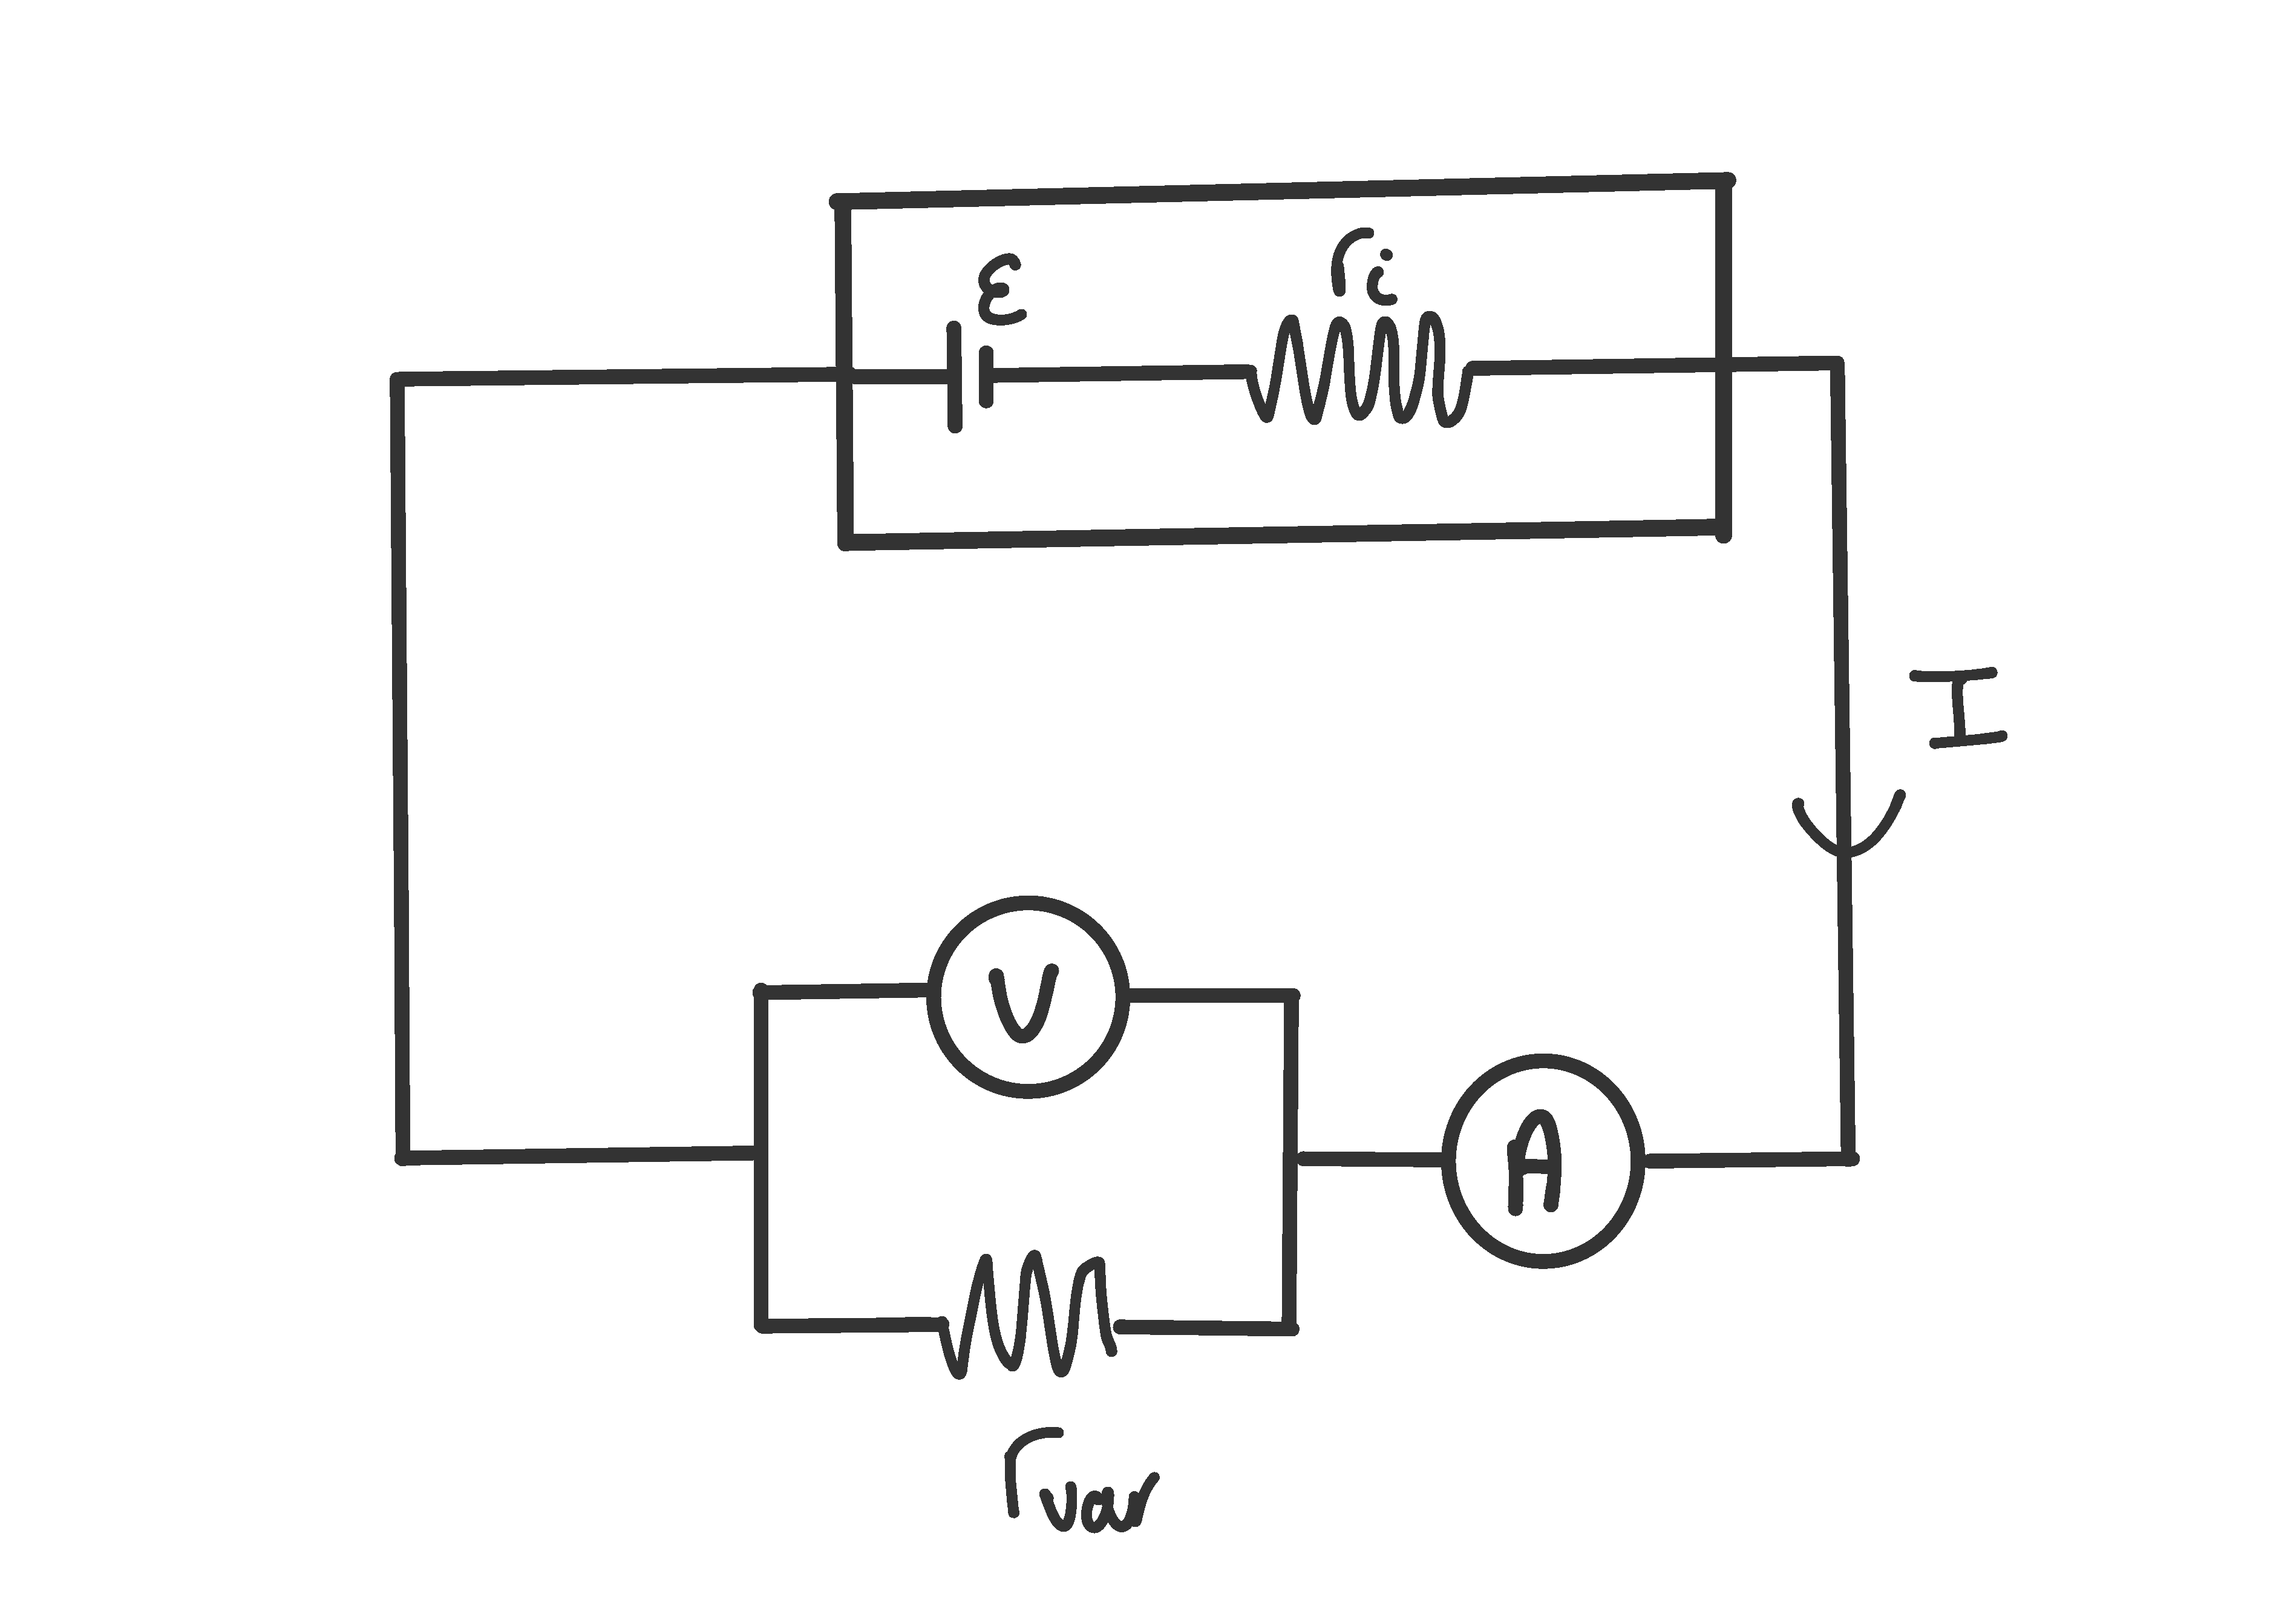
\includegraphics[scale=0.2]{montaje.png}
\caption{Montaje experimental para calcular $\varepsilon$. }
\label{Fig:montaje1}
\end{figure}


Una vez hemos obtenido tanto $T_2^{\infty}$ como $W_{RC}$, podemos obtener el valor de $\lambda_T$, ya que usando la ecuación \ref{Ec:lambda}:

\begin{equation}
\lambda_T = \dfrac{W_{RC}}{T_2^{\infty}-T_1} = \dfrac{W_{R_c}}{\Delta T}
\end{equation}


y usando la ecuación \ref{Ec:asociaciondeC}, como ya hemos calculado $\lambda_T$:

\begin{equation}
C_a = \dfrac{\lambda_T}{C}
\end{equation}

Haremos todo este proceso dándole los voltajes $V_0=125,150 V$ a la resistencia calefactora, por lo que obtendremos 2 capacidades caloríficas, 2 coeficientes de fourier y 2 valores para la resistencia interna $r_i$ del dispositivo. Además obtendremos un par de valores de $\varepsilon$ y $\Delta T$ diferentes que nos permitirá calcular dos coeficientes de Seebeck. 


\subsubsection{Segundo día:}

Como ya hemos mencionado, trataremos de calcular el valor del coeficiente Peltier. Para esto necesitamos conocer el valor del calor de Peltier que capta nuestra unión caliente. Sin embargo, para conocer dicho valor, antes que nada tenemos que hacer que la corriente circule en el sentido que nosotros requerimos para que realmente el efecto Peltier capte calor del entorno. Entonces lo primero que haremos nada mas llegar al laboratorio será hacer circular una corriente (de $1A$ mas o menos) a través del dispositivo termoeléctrico,y mediante un termómetro estudiar la evolución de su temperatura. Si aumenta tendremos que cambiar el sentido de circulación de la corriente (con cambiar la posición de los cables conectados al generador llega), y si disminuye la temperatura, ya tenemos el sentido de la corriente que buscamos, quedando el dispositivo tal y como la figura \ref{Fig:foto8}. \\



Una vez lo hemos determinado fijaremos la intensidad a $I=0.5A$, y el voltaje del generador a $V_0 = 120 V$. Para determinar que ambas medidas permanecen constantes a lo largo de la evolución a un estacionario tendremos tendremos dos polímetros (uno en función amperímetro, y otro en función voltímetro), que nos permitirá calcular ambos valores. Una vez fijamos la intensidad y el voltaje el sistema comenzará a evolucionar, en el primer caso, como la intensidad es baja y el voltaje muy alto, aumentando la temperatura. Entonces con el termómetro digital anotamos las temperaturas $T_1$ y $T_2$ cada minuto, hasta que $T_2$ no aumente mas de $0.1 C^o$ en 2 minutos, momento que podremos suponer un estado casi estacionario, y como tendremos los suficientes datos podremos hacer la regresión exponencial \ref{Ec:regresionexponecial} para calcular $T_2^{\infty}$. Como antes, $T_1$ la calcularemos suponiéndola constante. \\

Una vez lleguemos a este estado estacionario reptetiremos lo mismo pero cada vez aumentado la intensidad, subiendo por cada nuevo estado $0.5A$. Como aumentaremos la intensidad y no cambiaremos el voltaje podemos suponer que con cada cambio la temperatura de la unión bajará, ya que según el efecto Seebeck si aumentamos la intensidad tiene que aumentar la cantidad de calor captado. \\

Tendremos que parar de hacer medidas una vez la unión llegue a los $8 C^o$, ya que a partir de ahi la condensación o incluso la congelación del agua puede ocurrir, lo cuál sería fatal para nuestro circuito. \\

Una vez que alcanzamos este punto para $V_0 =120V$, repetiremos el proceso para $V_0 = 150 V$, comenzando de nuevo con $I=0.5 A$, por lo que volverá a aumentar la temperatura y, de nuevo, deberemos tomar datos de la temperatura y el tiempo; y luego hacer la regresión exponencial. 












\newpage

\section{Propagación de incertidumbres}

\subsection{Primer día}

Vamos a calcular las incertidumbres de $C_a$, $\lambda_T$, $S$, $\Delta T$, y $W_{R_c}$, que son, basándonos en las ecuaciones anteriores:

\begin{equation}
s(W_{R_c}) = \ccorchetes{\parentesis{\dfrac{2V}{R_c}}^2 s^2(V)+
\parentesis{\dfrac{V^2}{R_C^2}}^2 s^2(R_c)}^{1/2}
\end{equation}


\begin{equation}
s(\lambda_T) = \ccorchetes{\parentesis{\dfrac{1}{\Delta T}}^2 s^2(W_{R_c})+  \parentesis{\dfrac{W_{R_c}}{(\Delta T)^2}}^2 s^2(\Delta T) }^{1/2}
\end{equation}


\begin{equation}
s(C_a) = \ccorchetes{\parentesis{\dfrac{1}{C}}^2 s^2(\lambda_T)+  \parentesis{\dfrac{\lambda_T}{C^2}}^2 s^2(C) }^{1/2}
\end{equation}

\begin{equation}
s(\Delta T) = \ccorchetes{s^2(T_2^{\infty})+s^2(T_1)}^{1/2}
\end{equation}

\begin{equation}
s(S) = \ccorchetes{\parentesis{\dfrac{1}{\Delta T}}^2 s^2(\epsilon)+  \parentesis{\dfrac{\epsilon}{(\Delta T)^2}}^2 s^2(\Delta T) }^{1/2}
\end{equation}

\subsection{Segundo día}

\begin{multline}
s(\dot{Q}_P) = \left[ \parentesis{\dfrac{2V}{R_c}}^2 s^2(V)+
\parentesis{\dfrac{V^2}{R_C^2}}^2 s^2(R_c)+(\Delta T)^2 s^2(\lambda_T) +\right. \\ \left.  + (\lambda_T)^2 s^2(\Delta T)
+ \parentesis{I r_i}^2  s^2(I) + \parentesis{\frac{I^2}{2}}^2 s^2(r_i) \right]^{1/2}
\end{multline}



\newpage

\section{Incertidumbres}

En esta sección explicaremos de donde vienen las incertidumbres que mas adelante usaremos. Todos los datos que aparecen en está práctica se han obtenido mediante aparatos electrónicos, véase un termómetro digital o un polímetro. Como sabemos, las distribuciones de frecuencia provenientes de un aparato eléctrico son distribuciones de probabilidad uniformes. Por lo tanto cogeremos para cada valor una incertidumbre igual a la precisión de nuestro aparato entre la raíz de doce, a no ser que oscilen entre varios valores. Por el contrario nosotros no solo usaremos está incertidumbre de tipo B basada en la distribución de frecuencias, si no que la aumentaremos hasta que llegue a la precisión del aparato. Lo hacemos así para incluir todas aquellas incertidumbres que no conocemos y que si afectan a los datos. Además muchos datos oscilaban. Para ser rigurosos deberíamos decir de donde extraemos cada incertidumbre, pero dicha rigurosidad excede la intención de la práctica. Siguiendo este razonamiento tendremos que:

\begin{itemize}
\item Cada temperatura medida tendrá una incertidumbre asociada de

\begin{equation}
s(T) = 0.1 C^o
\end{equation}

\item Cada valor de voltaje, intensidad, o resistencia medida tendrá un valor igual a la precisión del aparato. Esta variará ya que no siempre tendrá la misma precisión el aparato: a veces mediremos voltajes grandes y otras veces algunos pequeños. Entonces:

\begin{itemize}
\item Resistencia $R_c$ directamente: $$s(R_c) = 10 \Omega$$
\item Voltaje para resistencia $R_c$: $$s(V_{R_c}) = 1 V$$
\item Intensidad para resistencia $R_c$: $$s(I_{R_c}) = 0.001A$$
\item Voltaje $V_0$: $$s(V_0) = 1 V$$.
\item Diferencia de potencial $\Delta V_{Rx}$: $$ s(\Delta V_{Rx}) = 0.001 V $$
\item Intensidad $I_{Rc}$: $$ s(I_{Rx}) = 0.1 mA $$
\item Intensidad para peltier: $$ s(I) = 0.01 A $$
\end{itemize}

Aunque hay que decir que realmente las incertidumbres reales no son esas, son meras aproximaciones. A dichas incertidumbres dadas por las distribuciones de frecuencia hay que añadir las especificaciones del fabricante.

\end{itemize}


\newpage

\section{Resultados experimentales}

\subsection{Calculo de $R_c$}


En la primera parte de esta práctica teníamos que calcular los valores de la resistencia de manera directa, de donde podemos obtener que

\begin{table}[h!] 	 \centering 
\begin{tabular}{|c|c|c|c|} 
\hline 
$ R_{C1} \ (\Omega)$ & $s(R_{C1}) \ (\Omega) $ & $R_{C2} \ (\Omega)$ & $ s(R_{C2}) \ (\Omega) $ \\ \hline 
1010  & 10 & 989 &  10 \\ 
\hline
\end{tabular} 
\caption{Valor para la resistencia $R_C$ calculada de manera directa} 
\label{tab:} 
\end{table} 

y de manera indirecta teníamos que obtener los pares de valores para hacer la regresión lineal 




\begin{table}[h!] 	 \centering 
\begin{tabular}{|c|c|c|c|} 
\hline 
$a \ (V)$ & $s(a) \ (V)$ & $R_{C3} \ (\Omega)$ & $s(R_{C3}) \ (\Omega)$  \\ \hline 
-4.45 & 0.71 &  1039.5& 5.7 \\ 
\hline
\end{tabular} 
\caption{valor de la resistencia y ordenada en el origen mediante la regresión lineal} 
\label{tab:} 
\end{table} 




\begin{figure}[h!] \centering
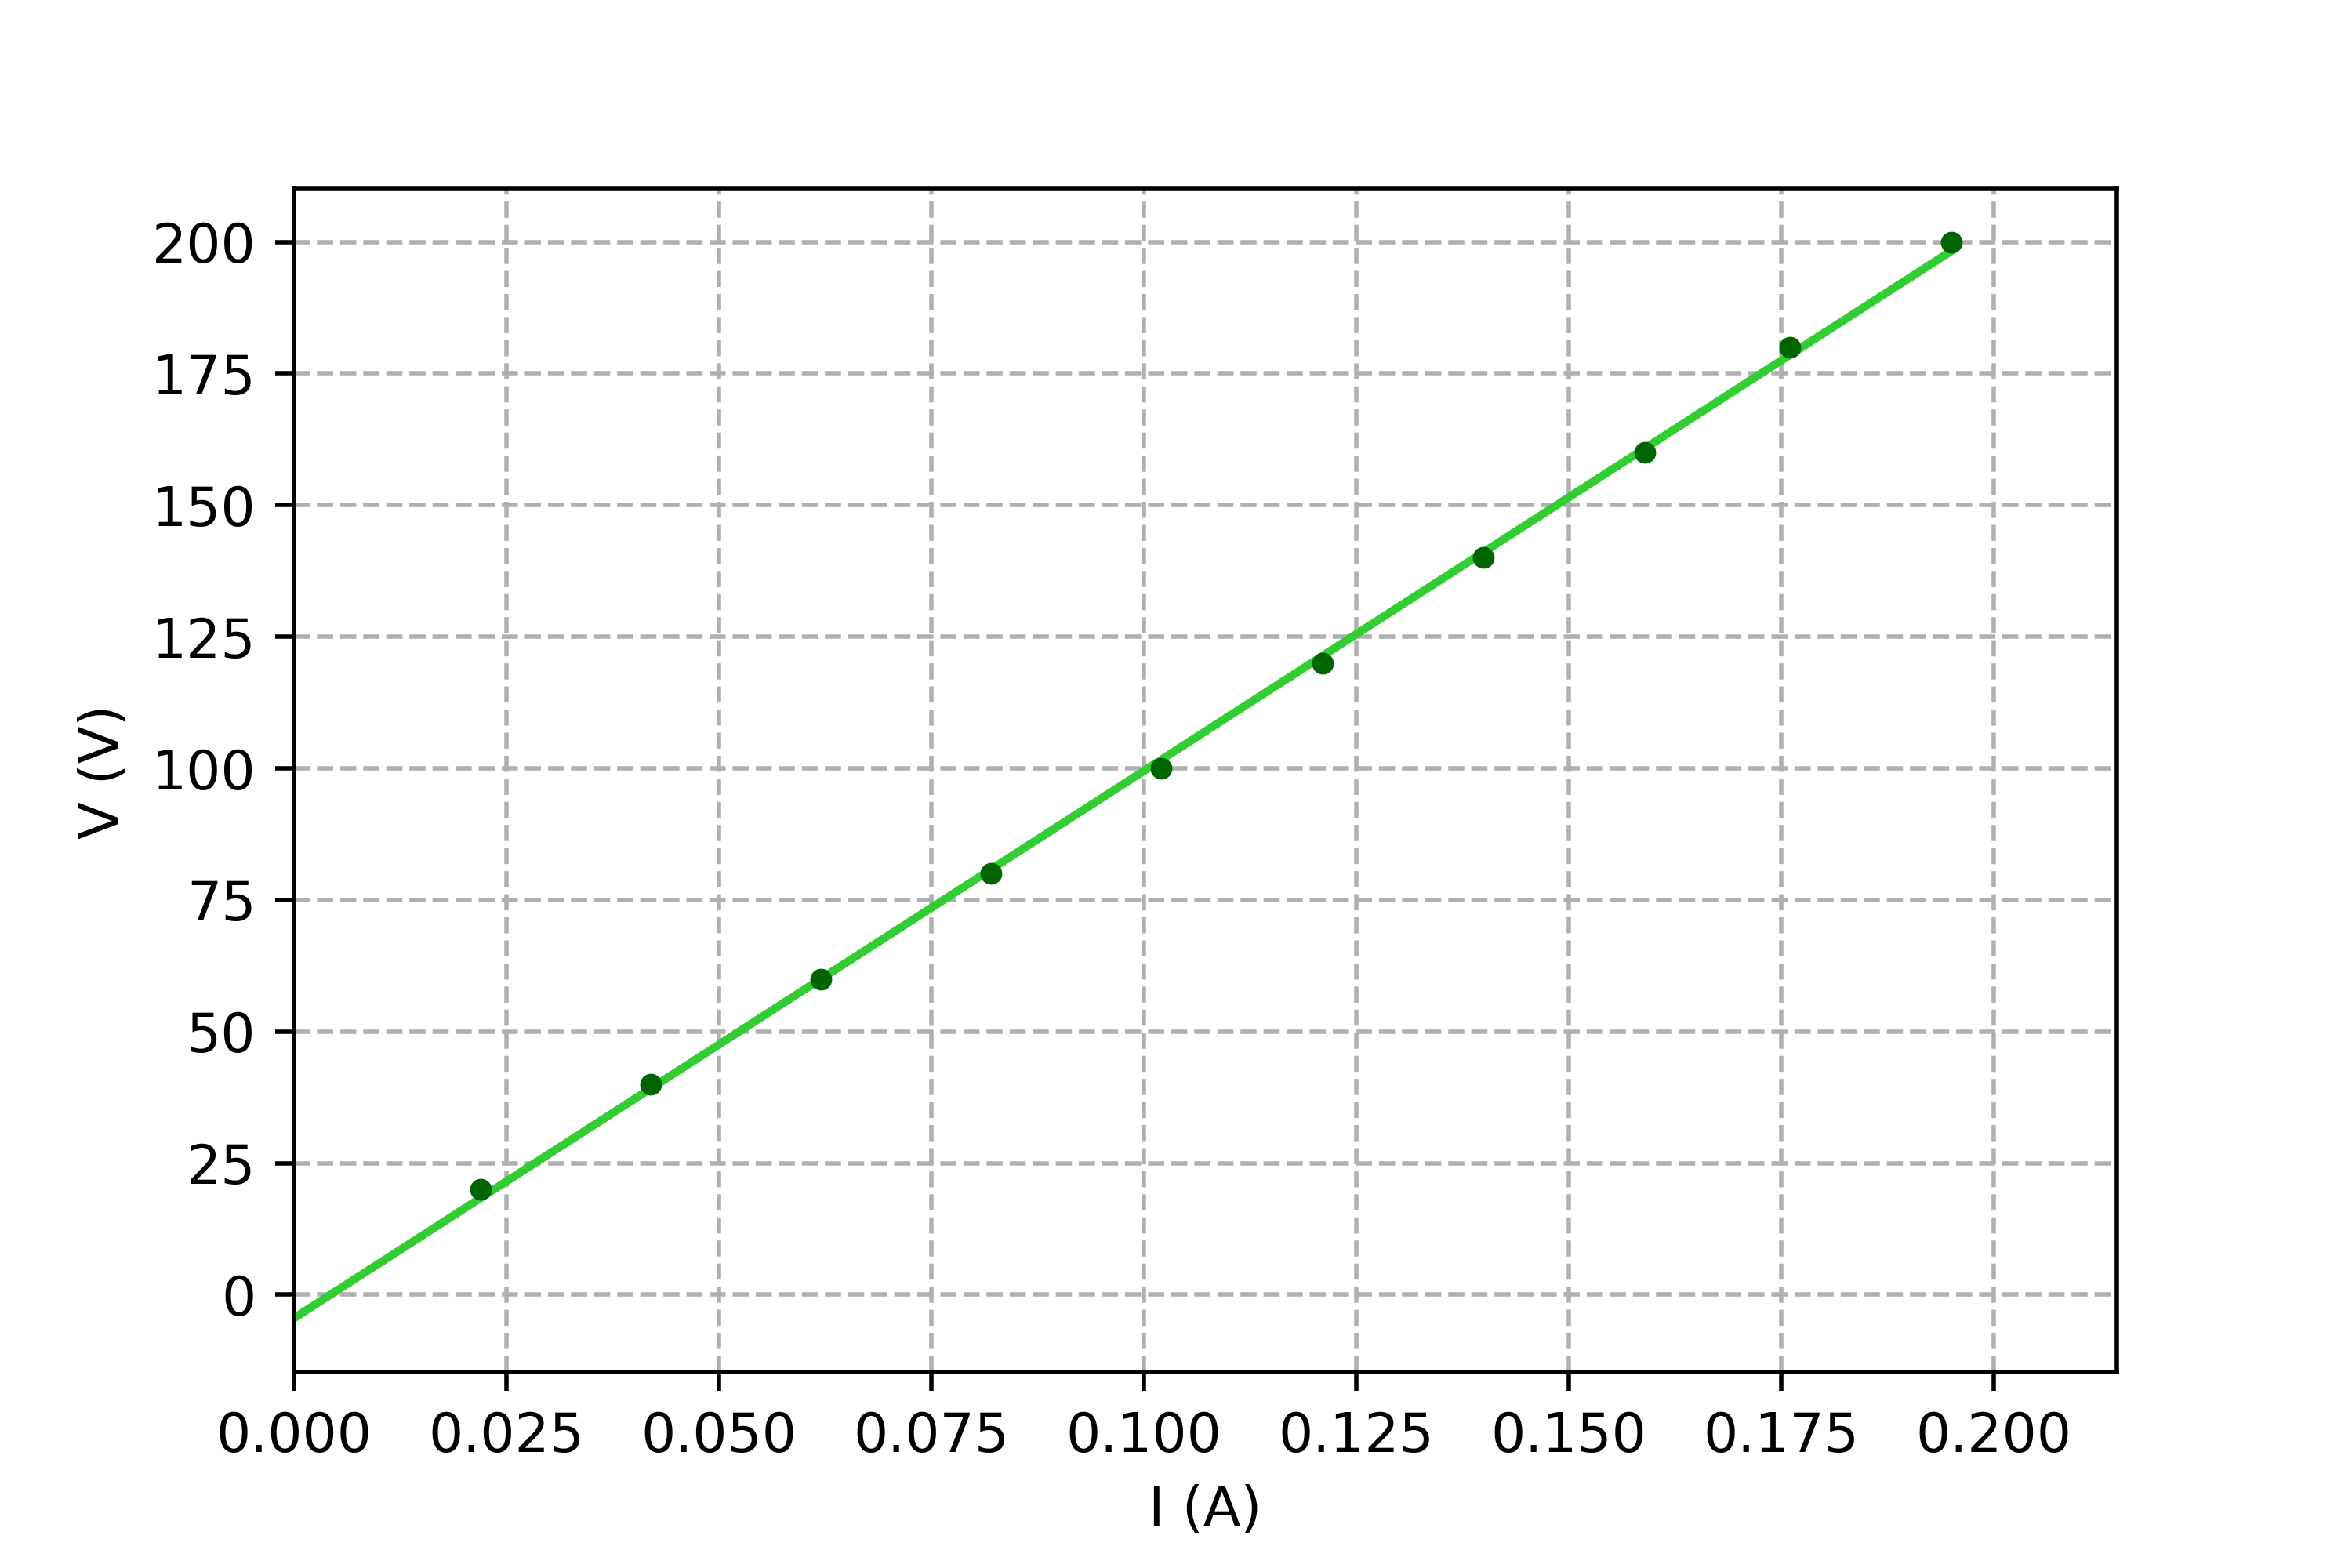
\includegraphics[scale=1]{R.png}
\caption{representación $V$ frente a $I$ para el cálculo de $R_C$}
\end{figure}



Entonces hemos obtenido 3 valores de la resistencia con 3 incertidumbres diferentes. Para obtener el valor definitivo haremos una media ponderada entre las 3. Entonces podemos concluir que:


\begin{table}[h!] 	 \centering 
\begin{tabular}{|c|c|} 
\hline 
 $R_C \ (\Omega)$ & $s(R_C) \ (\Omega)$  \\ \hline 
1023.7  & 4.4  \\ 
\hline
\end{tabular} 
\caption{valor de la resistencia final} 
\label{tab:} 
\end{table} 


\newpage



\subsection{Calculo de valores térmicos}


En la tabla \ref{tab:04} podemos ver la media de las temperaturas de la unión fría. Aunque a lo largo de la práctica la temperatura del agua varíe (ya que la temperatura de las cañerías asciende a medida que avanza el día) supondremos que se encontraba constante con los valores allí representados. La incertidumbre fue calculada mediante una mezcla entre la incertidumbre del aparato ($u_b$) siendo esta la incertidumbre de la media ponderada y mediante la inferencia estadística de la media ($u_a$), pero dado el peso de está última, la primera puede considerarse ridículamente pequeña. Para hacer esto hemos supuesto:


\begin{equation}
u_c = \parentesis{u_a^2 + u_b^2}^{1/2} 
\end{equation}

\begin{table}[h!] 	 \centering 
\begin{tabular}{|c|c||c|c|} 
\hline 
$ T_1^1  \ (C^o)$ & $s( T_1^1) \ (C^o)$  & $ T_1^2  \ (C^o)$ & $s( T_1^2) \ (C^o) $ \\ \hline  
 12.489 &  0.041 &  13.478  & 0.026 \\ \hline 
\end{tabular} 
\caption{Valores de la temperatura unión fría para $V_0 = 125 \ V$ ($ T_1^1$) y $V_0 = 150 \ V$ ($ T_1^2$)} 
\label{tab:04} 
\end{table} 


En las tablas \ref{tab:05} y \ref{tab:06} están representados los valores con sus incertidumbres al realizar el ajuste exponencial de los datos $T_2$ respecto al tiempo. Como podemos ver según las ecuaciones mencionadas anteriormente $T_2^{\infty} = A$. Las regresiones han sido calculadas con el módulo scipy.optimize, que usa puro cálculo numérico para obtenerlas, por lo que es posible que exista algún error mínimo en los datos. Las incertidumbres expuestas en la tabla son las incertidumbres de tipo A, ya que podríamos considerar las incertidumbres de tipo B prácticamente nulas al no saber con certeza cual es la distribución de frecuencias de cada dato en particular. 


\begin{table}[h!] 	 \centering 
\begin{tabular}{|c|c|c|c|c|c|} 
\hline 
$A \ (C^o)$ & $s(A) \ (C^o)$ & $ B  \ (C^o)$ & $s(B) \ (C^o)$ &$ C \ (\mathrm{min}^{-1})$ & $ s(C) \ (\mathrm{min}^{-1}) $ \\ \hline 
29.586  & 0.018 &  -13.305153 & 0.020 & 0.05262400 & 0.0000029 \\ 
\hline
\end{tabular} 
\caption{Valores obtenidos de las regresiones exponenciales para $V_0 = 125 V$} 
\label{tab:05} 
\end{table} 

\begin{table}[h!] 	 \centering 
\begin{tabular}{|c|c|c|c|c|c|} 
\hline 
$A \ (C^o)$ & $s(A) \ (C^o)$ & $ B  \ (C^o)$ & $s(B) \ (C^o)$ & $C \ (\mathrm{min}^{-1})$ &  $s(C) \ (\mathrm{min}^{-1}) $ \\ \hline 
36.0033  & 0.0012 &  -7.4166 & 0.0017 & 0.07291000 & 0.0000014 \\ 
\hline
\end{tabular} 
\caption{Valores obtenidos de las regresiones exponenciales para $V_0 = 150V$} 
\label{tab:06} 
\end{table} 

En la tabla \ref{tab:07} están puestas las diferencias de temperaturas $T_2^{\infty}-T_1$, tomando los valores de estos en las tablas anteriores. Para calcular la incertidumbre de los siguientes datos solo tendremos en cuenta la propagación de incertidumbres, ya que no tenemos ningún tipo de incertidumbre de tipo B a mayores para añadir. \\
 



En las siguientes tablas se muestran los datos recogidos de los coeficientes $W_{R_C}$, $\lambda_T$ y $C_a$, en primer lugar para el primer estacionario, en el segundo para el segundo estacionario, y a la derecha la media ponderada para los 3 coeficientes que tomaremos como constantes a lo largo del segundo día. Sobre las incertidumbres, sucede lo mismo que en las dos anteriores. \\


\begin{table}[h!] 	 \centering 
\begin{tabular}{|c|c|c|c|} 
\hline 
$\Delta T_1  \ (C^o)$ & $s(\Delta T_1) \ (C^o)$  & $\Delta T_2  \ (C^o)$ & $s(\Delta T_2) \ (C^o) $ \\ \hline  
 17.096 &  0.044 &  22.525 & 0.026 \\ \hline 
\end{tabular} 
\caption{Valores de $\Delta T$ para $V_0 = 125 \ V$ ($\Delta T_1$) y $V_0 = 150 \ V$ ($\Delta T_2$)} 
\label{tab:07} 
\end{table} 

\begin{table}[h!] 	 \centering 
\begin{tabular}{|c|c|c|c||c|c|} 
\hline 
 $W_{R_c}^1 \ (J)$ & $s(W_{R_c}^1) \ (J)$ & $W_{R_c}^2 \ (J)$  & $s(W_{R_c}^2) \ (J) $ & $W_{R_c} \ (J)$ & $s(W_{R_c}) \ (J)$ \\ \hline 
 15.26 & 0.25 & 21.98 & 0.31 & 17.97 & 0.20 \\ 
\hline
\end{tabular} 
\caption{Valores de $W_{R_c}$ para $V_0 = 125 \ V$ ($W_{R_c}^1$) y $V_0 = 150 \ V$ ($W_{R_c}^2$)} 
\label{tab:} 
\end{table} 


\begin{table}[h!] 	 \centering 
\begin{tabular}{|c|c|c|c||c|c|} 
\hline 
 $\lambda_T^1 \ (W/C^o)$ & $s(\lambda_T^1 ) \ (W/C^o)$  & $\lambda_T^2 \ (W/C^o)$  & $s(\lambda_T^2) \ (W/C^o) $ & $\lambda_T \ (W/C^o)$ & $s(\lambda_T) \ (W/C^o)$ \\ \hline 
 0.893 & 0.015 & 0.976 & 0.014 & 0.938 & 0.010 \\ 
\hline
\end{tabular} 
\caption{Valores de $\lambda_T$ para $V_0 = 125 \ V$ ($\lambda_T^1$) y $V_0 = 150 \ V$ ($\lambda_T^2$)} 
\label{tab:} 
\end{table} 


\begin{table}[h!] 	 \centering 
\begin{tabular}{|c|c|c|c||c|c|} 
\hline 
 $C_a^1 \ (J/C^o)$ & $s(C_a^1 ) \ (J/C^o)$  & $C_a^2 \ (J/C^o)$  & $s(C_a^2) \ (J/C^o) $ & $C_a \ (J/C^o)$ & $s(C_a) \ (J/C^o)$ \\ \hline 
 1018 & 17 & 803 & 11 & 868.4 & 9.4 \\ 
\hline
\end{tabular} 
\caption{Valores de $C_a$ para $V_0 = 125 \ V$ ($C_a^1$) y $V_0 = 150 \ V$ ($C_a^2$)} 
\label{tab:} 
\end{table} 






\begin{figure}[h!] \centering
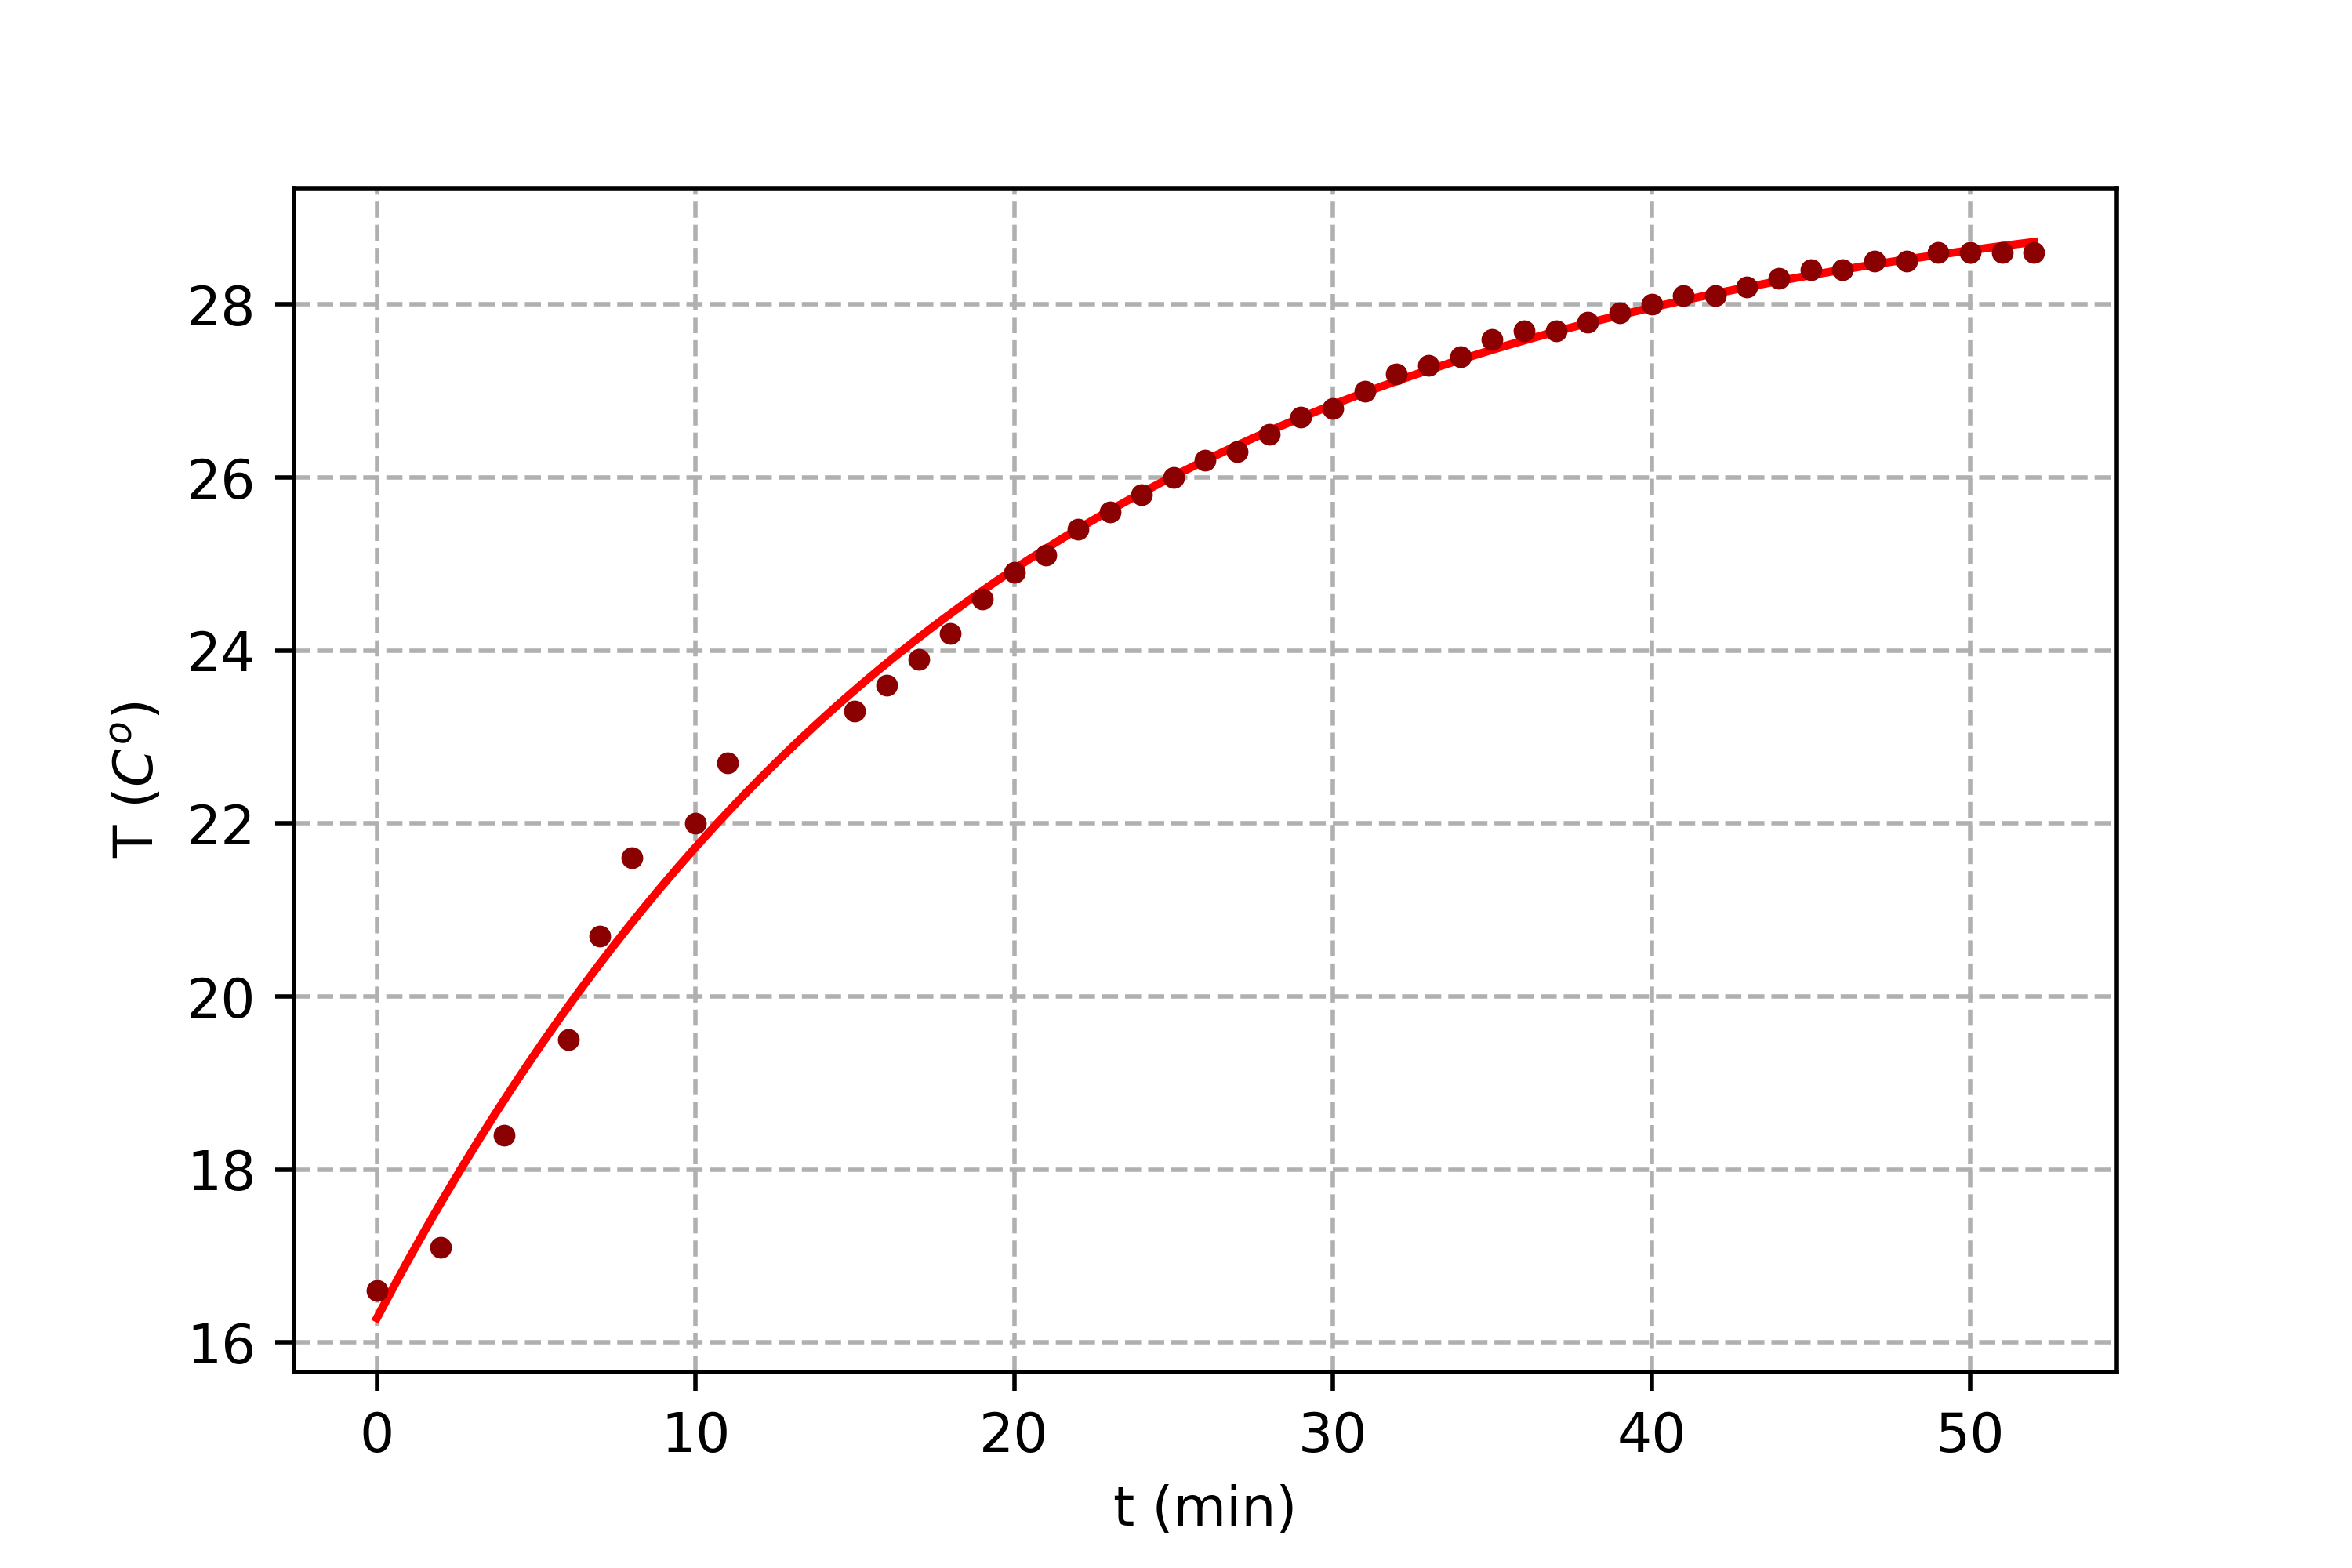
\includegraphics[scale=0.9]{T1.png}
\caption{representación $T_2$ frente a $t$ con la regresión para $V=125V$}
\end{figure}

\begin{figure}[h!] \centering
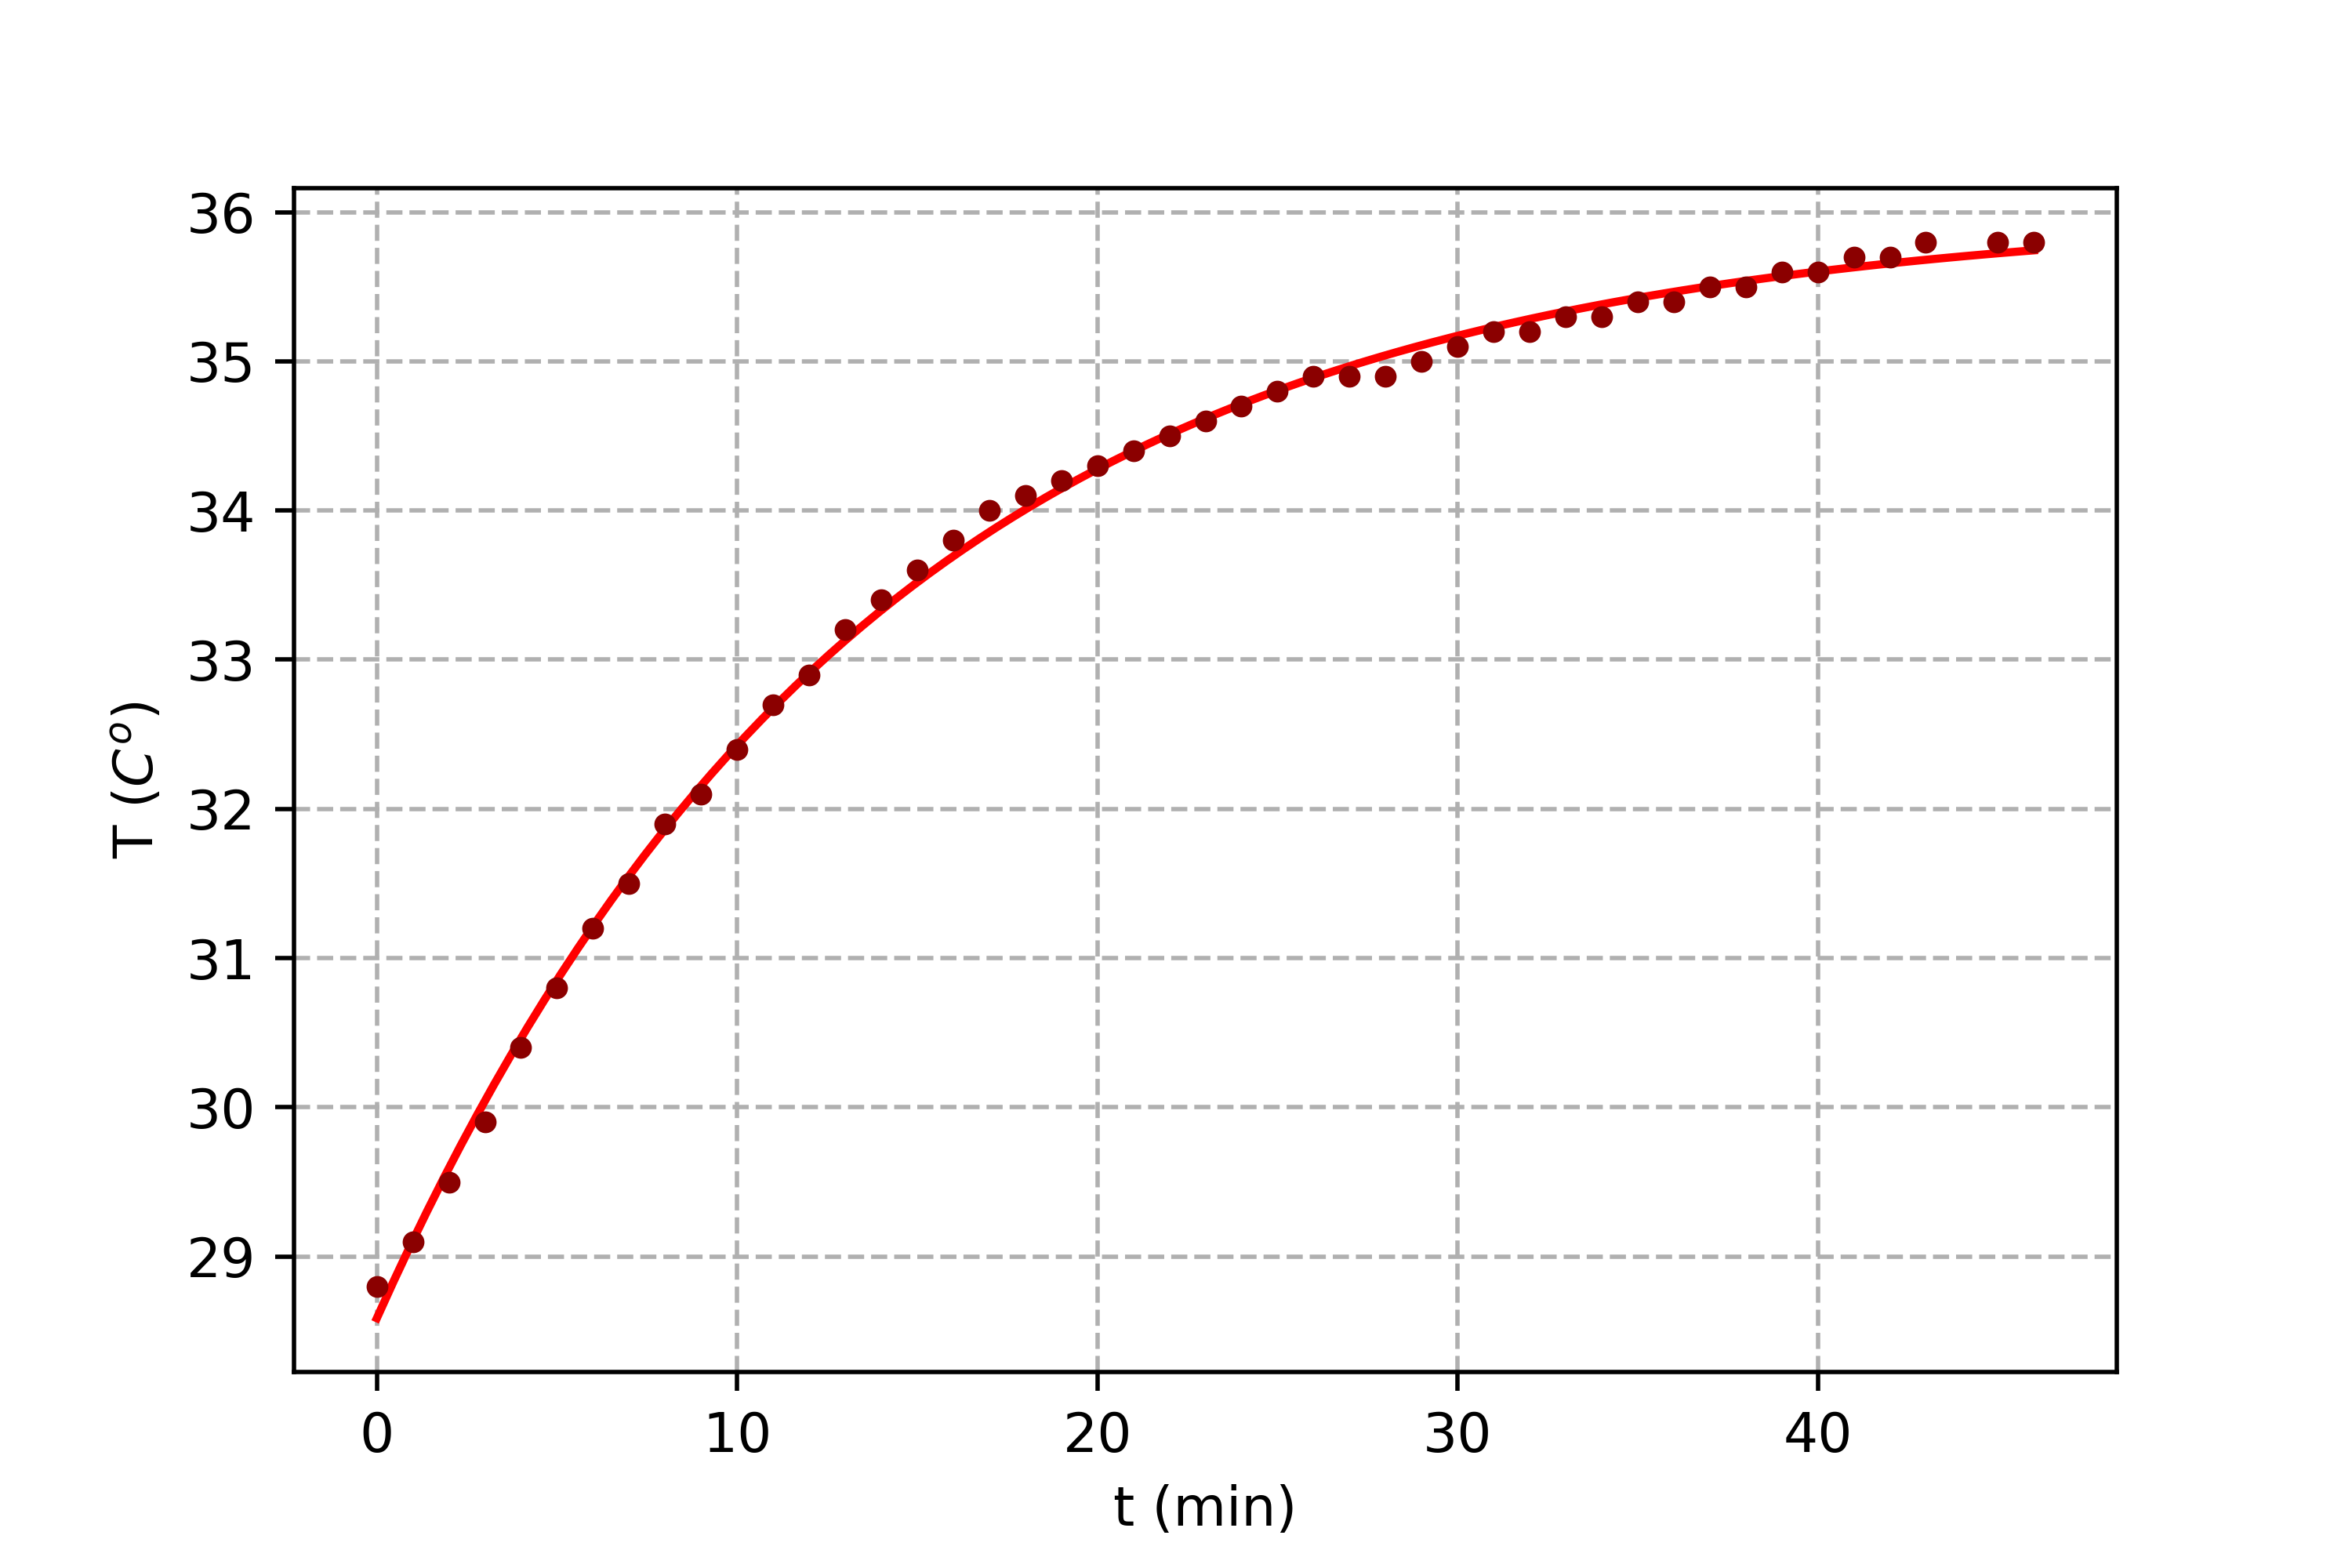
\includegraphics[scale=0.9]{T2.png}
\caption{representación $T_2$ frente a $t$ con la regresión para $V=150V$}
\end{figure}



\newpage

\subsection{Calculo de los potenciales en estado estacionario}




En las tablas \ref{tab:11} y \ref{tab:12} están representadas los potenciales calculados de forma directa (\ref{tab:11}) y de forma indirecta (\ref{tab:12}), incluyéndose en la segunda tabla el valor de la resistencia $r_i$ para el primer estado estacionario. No hay nigún tipo de dificultad en el cálculo de ambos ya que en el primer caso es una medida directa y como ya hemos explicado, tiene como incertidumbre de la precisión del aparato; y en el segundo caso son las incertidumbres de tipo A que se obtienen al hacer una regresión lineal normal. No incluimos en este caso otra incertidumbre de tipo B.  Las tablas  \ref{tab:13} y \ref{tab:14} reflejan exactamente lo mismo para el segundo estacionario.



\begin{table}[h!] 	 \centering 
\begin{tabular}{|c|c|} 
\hline 
$\varepsilon \ (V)$ & $s(\varepsilon) \ (V) $ \\ \hline 
0.855000  & 0.0010 \\ 
\hline
\end{tabular} 
\caption{Valores para la fuerza electromotriz V=125V de manera directa} 
\label{tab:11} 
\end{table} 


\begin{table}[h!] 	 \centering 
\begin{tabular}{|c|c|c|c|} 
\hline 
$\varepsilon \ (V)$ & $s(\varepsilon) \ (V)$ & $r_i \ (\Omega)$ & $r_i \ (\Omega)$  \\ \hline
0.8410  & 0.0014 &  -7.926 & 0.019 \\ 
\hline
\end{tabular} 
\caption{Valores para la fuerza electromotriz y la resistencia V=125V mediante ajuste lineal} 
\label{tab:12}
\end{table}



\begin{table}[h!] 	 \centering 
\begin{tabular}{|c|c|} 
\hline 
$\varepsilon \ (V)$ & $s(\varepsilon) \ (V) $ \\ \hline 
1.1950  & 0.0010 \\ 
\hline
\end{tabular} 
\caption{Valores para la fuerza electromotriz  V=150V de manera directa} 
\label{tab:13} 
\end{table} 

\begin{table}[h!] 	 \centering 
\begin{tabular}{|c|c|c|c|} 
\hline 
$\varepsilon \ (V)$ & $s(\varepsilon) \ (V)$ & $r_i \ (\Omega)$ & $r_i \ (\Omega)$  \\ \hline
1.2008  & 0.0013 &  -7.994 & 0.013 \\ 
\hline
\end{tabular} 
\caption{Valores para la fuerza electromotriz y la resistencia V=150V mediante ajuste lineal} 
\label{tab:14} 
\end{table}


En la tabla \ref{tab:15} se muestra la media ponderada para cada uno de los valores de la fuerza electromotriz entre la medida directa e indirecta. Es esencial para calcular el coeficiente Seebeck ($S$). En la tabla \ref{tab:16} se ve cual es la media ponderada de los valores de la resistencia intrínseca del dispositivo, que usaremos para la parte de Peltier.

\begin{table}[h!] 	 \centering 
\begin{tabular}{|c|c|c|c|} 
\hline 
$\varepsilon^1  \ (V)$ & $s(\varepsilon^1) \ (V)$  & $\varepsilon^2  \ (V)$ & $s(\varepsilon^2) \ (V) $ \\ \hline  
 0.85044 &  0.00082 &  1.19658 & 0.00070 \\ \hline 
\end{tabular} 
\caption{Valores de $\varepsilon$ para $V_0 = 125 \ V$ ($\varepsilon^1$) y $V_0 = 150 \ V$ ($\varepsilon^2$)} 
\label{tab:15} 
\end{table} 

\begin{table}[h!] 	 \centering 
\begin{tabular}{|c|c|}
\hline 
$r_i  \ (\Omega)$ & $s(r_i) \ (\Omega)$ \\ \hline  
 7.972 &  0.011 \\ \hline 
\end{tabular} 
\caption{Valores de $r_i$ definitivos tras hacer la media ponderada}
\label{tab:16} 
\end{table} 





\begin{figure}[h!] \centering
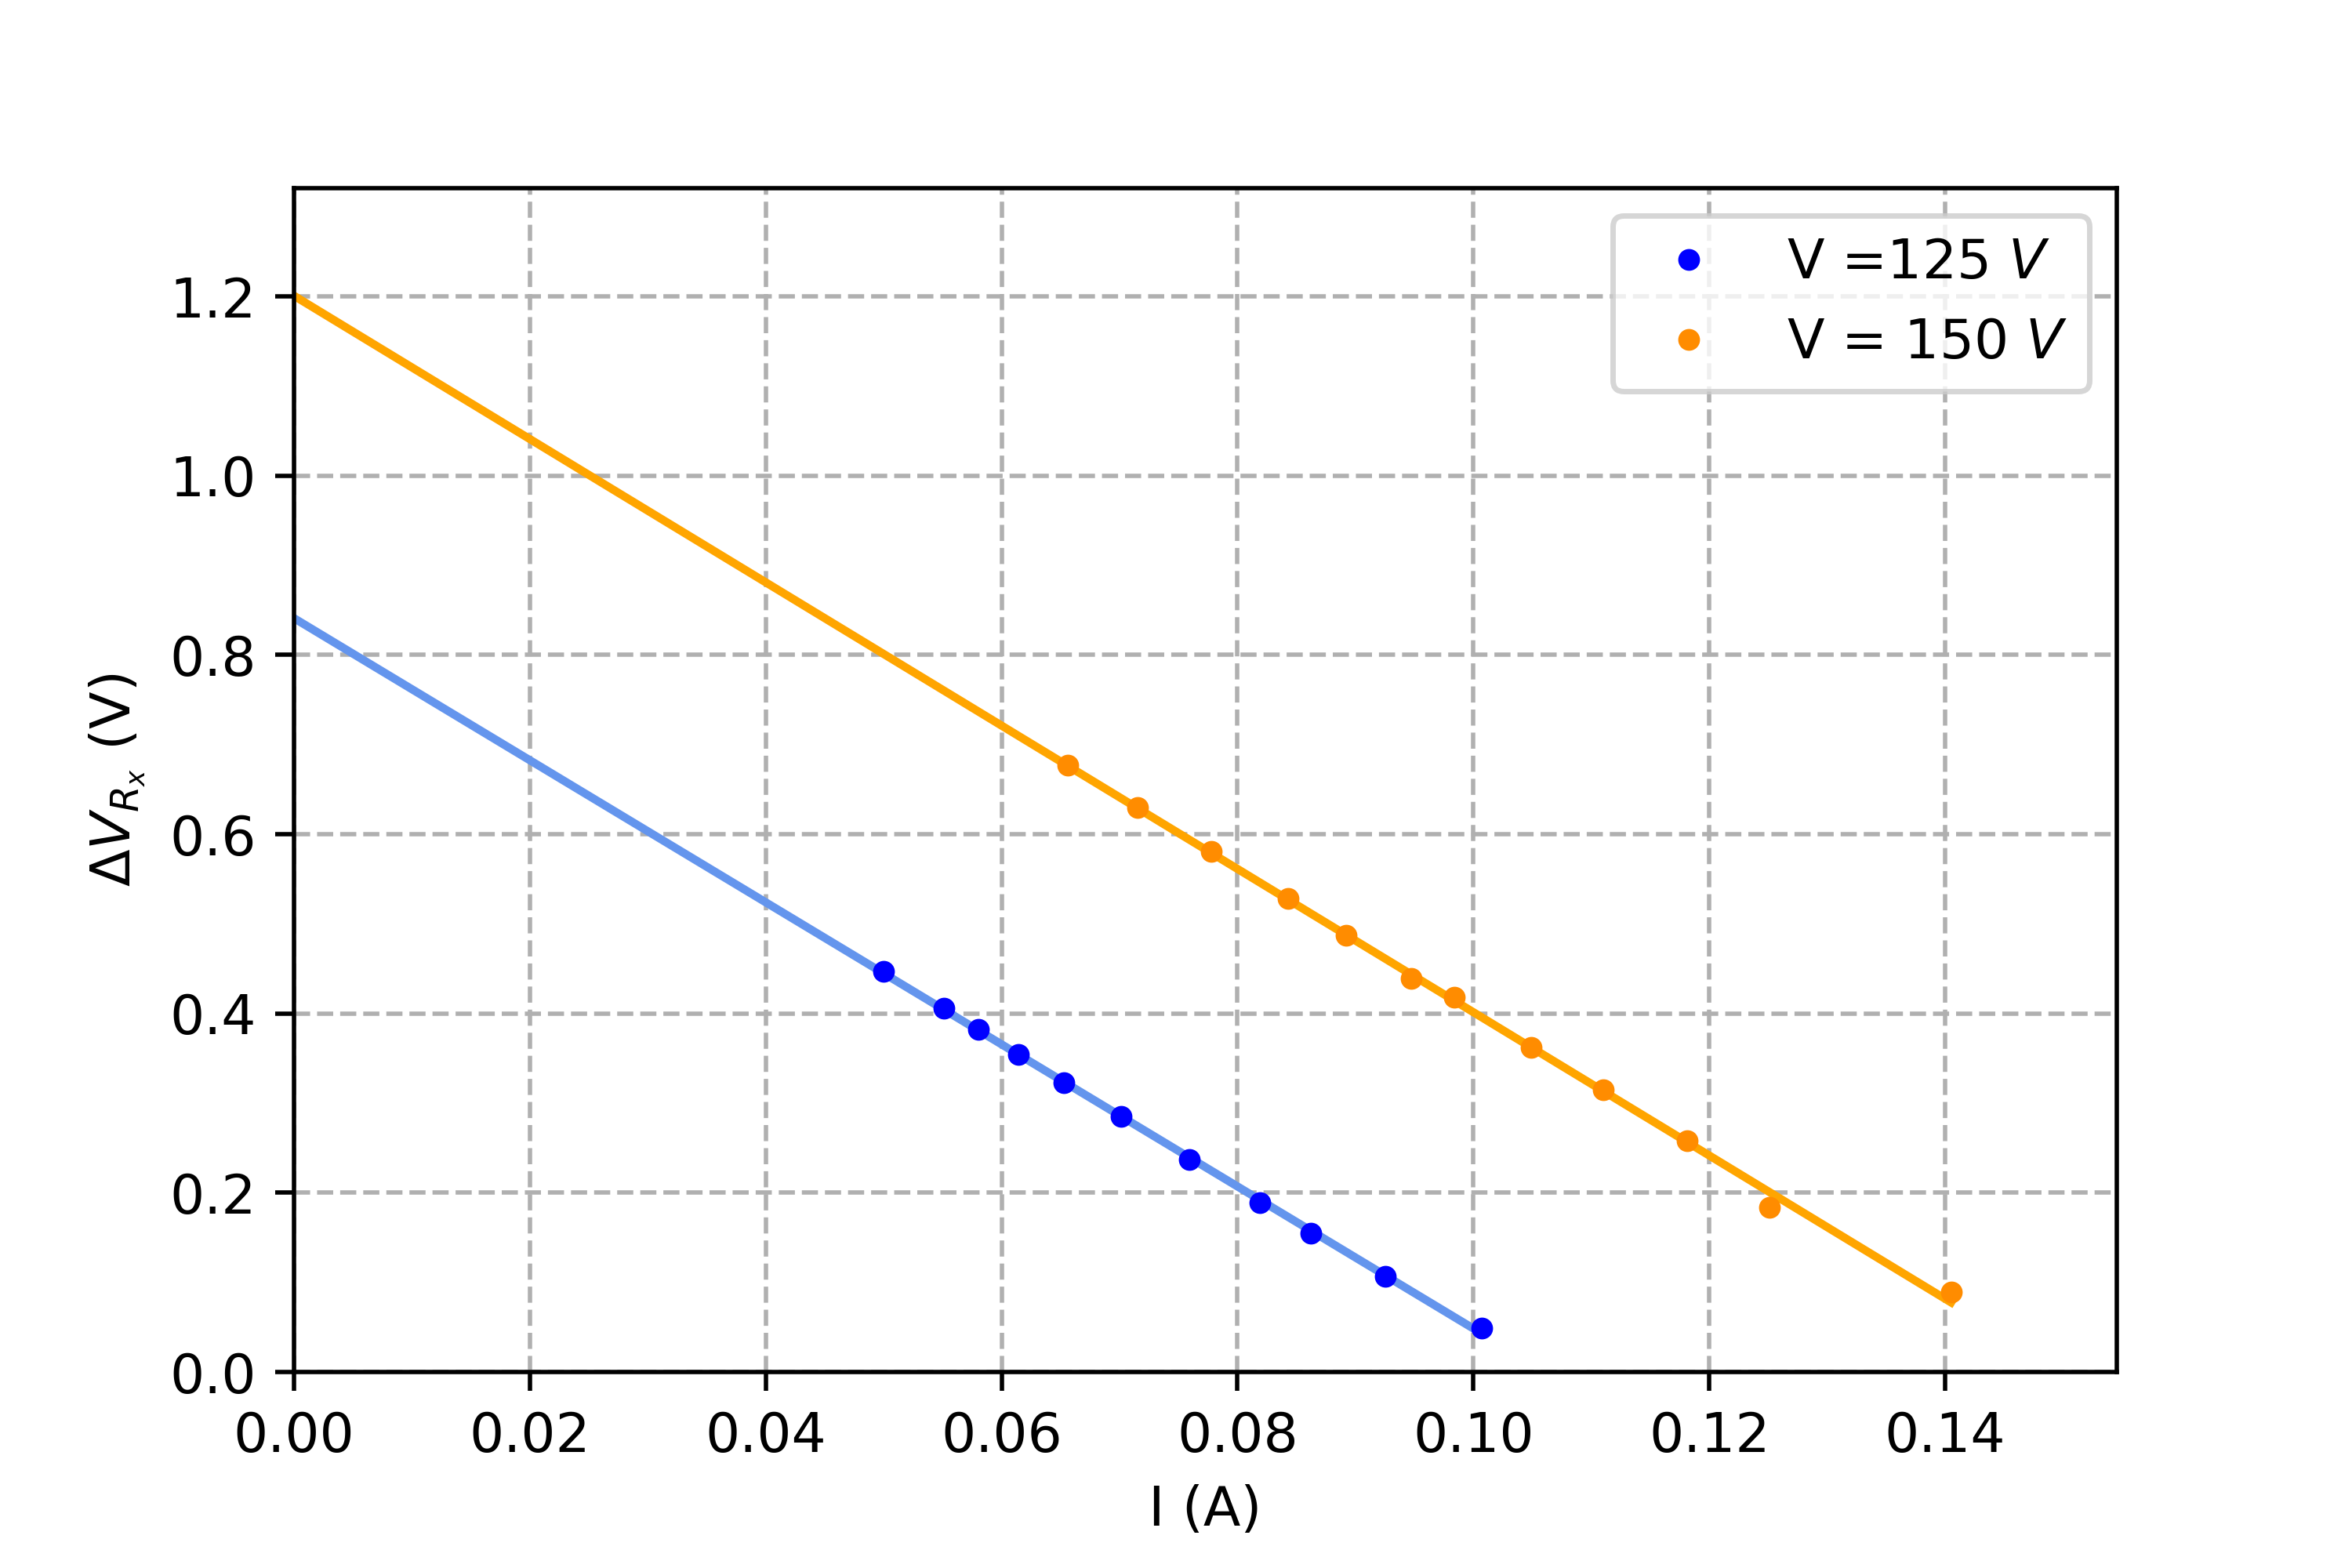
\includegraphics[scale=1]{I-vs-V.png}
\caption{V=125,150 V}
\end{figure}



\subsection{Coeficiente Seebeck}


En la siguiente tabla (tabla \ref{tab:17}) tenemos los dos coeficientes Seebeck para cada uno de los dos voltajes y luego su media ponderada. El segundo valor es el resultado final de toda la práctica, y en última instancia, el valor que queríamos obtener. La incertidumbre la calculamos mediante la fórmula de propagación de incertidumbres normal, no añadiremos ningún tipo de incertidumbre a mayores para combinar, ya que tampoco conocemos cual es su distribución de datos. 

\begin{table}[h!] 	 \centering 
\begin{tabular}{|c|c|c|c||c|c|} 
\hline 
 $S^1 \ (V/C^o)$ & $s(S^1 ) \ (V/C^o)$  & $S^2 \ (V/C^o)$  & $s(S^2) \ (V/C^o) $ & $S \ (V/C^o)$ & $s(S) \ (V/C^o)$ \\ \hline 
 0.049744 & 0.00014 & 0.053122 & 0.000069 & 0.052441 & 0.000062 \\ 
\hline
\end{tabular} 
\caption{Valores de $S$ para $V_0 = 125 \ V$ ($S^1$) y $V_0 = 150 \ V$ ($S^2$)} 
\label{tab:17} 
\end{table} 


\subsection{Calor Peltier}

Como ya hemos dicho al principio de la memoria, el primer día hicimos muchos cálculos que no eran necesarios para el cálculo del coeficiente Seebeck, pero si para el cálculo del coeficiente Peltier. Estos erán $\lambda_T$, $r_i$ y $R_c$. Entonces los valores que usaremos a lo largo de está parte de la práctica serán:

\begin{equation}
\begin{array}{lllllll}
\lambda_T & = & 0.938  \ W/C^o & \ \ & s(\lambda_T) & = & 0.010  \ W/C^o \\
R_c & = & 1023.4 \ \Omega \ & \ \ & s(R_c) & = & 4.4 \ \Omega \\
r_i & = & 7.972 \ \Omega  & \ \ & s(r_i) & = & 0.011 \ \Omega
\end{array}
\end{equation}


He de recordar que los valores de todas las regresiones lineales presentadas en esta sección se encuentran en la parte final de la memoria ya que ponerlas aquí ejercería un efecto visual negativo, y dado que solo tomamos un dato de ellas, no son lo suficientemente importantes como para ponerlas a pesar de eso. 

\subsubsection{Estacionario 1}
En este estacionario hemos seleccionado las siguientes magnitudes de intensidad y voltaje  
\begin{equation} 
\begin{array}{lllllll}
I & = & 0.53 A & \ \ & s(I) & = & 0.01  A \\ 
 V_0 & = & 120 V & \ \ & s(V_0) & = & 1 V
\end{array} 
\end{equation} 
 Haciendo el ajuste exponencial (fig \ref{Fig:graficapeltier1}) y la media de al tempertatura del foco frío obtenemos que para el valor estacionario las temperaturas serán: 
\begin{equation} 
\begin{array}{lllllll}
T_2^{\infty} & = & 21.7752 C^o &  \ \ &  s(T_2^{\infty}) & =  & 0.0030  C^o \\ 
 T_1 & = & 14.476  C^o & \ \ & s(T_1) & = & 0.034  C^o \\ 
 \end{array} 
\end{equation} 
 Por lo tanto, teniendo en cuenta los datos anteriores, y los que proceden de la anterior práctica, tenemos que en este caso el calor peltier será: 
\begin{equation} 
\begin{array}{lllllll}
\dot{Q}_P & = & 8.32 J & \ \ & s(\dot{Q})_P & = & 0.26 J \\ 
\end{array} 
\end{equation} 
 

\newpage
 
 
\subsubsection{Estacionario 2}
En este estacionario hemos seleccionado las siguientes magnitudes de intensidad y voltaje  
\begin{equation} 
\begin{array}{lllllll}
I & = & 1.00 A & \ \ & s(I) & = & 0.01  A \\ 
 V_0 & = & 120 V & \ \ & s(V_0) & = & 1 V
\end{array} 
\end{equation} 
 Haciendo el ajuste exponencial (fig \ref{Fig:graficapeltier2}) y la media de al tempertatura del foco frío obtenemos que para el valor estacionario las temperaturas serán: 
\begin{equation} 
\begin{array}{lllllll}
T_2^{\infty} & = & 15.7675 C^o &  \ \ &  s(T_2^{\infty}) & =  & 0.0093  C^o \\ 
 T_1 & = & 15.093  C^o & \ \ & s(T_1) & = & 0.040  C^o \\ 
 \end{array} 
\end{equation} 
 Por lo tanto, teniendo en cuenta los datos anteriores, y los que proceden de la anterior práctica, tenemos que en este caso el calor peltier será: 
\begin{equation} 
\begin{array}{lllllll}
\dot{Q}_P & = & 17.43 J & \ \ & s(\dot{Q})_P & = & 0.26 J \\ 
\end{array} 
\end{equation} 
 
 
 
 
\subsubsection{Estacionario 3}
En este estacionario hemos seleccionado las siguientes magnitudes de intensidad y voltaje  
\begin{equation} 
\begin{array}{lllllll}
I & = & 1.52 A & \ \ & s(I) & = & 0.01  A \\ 
 V_0 & = & 120 V & \ \ & s(V_0) & = & 1 V
\end{array} 
\end{equation} 
 Haciendo el ajuste exponencial (fig \ref{Fig:graficapeltier3}) y la media de al tempertatura del foco frío obtenemos que para el valor estacionario las temperaturas serán: 
\begin{equation} 
\begin{array}{lllllll}
T_2^{\infty} & = & 10.3475 C^o &  \ \ &  s(T_2^{\infty}) & =  & 0.0043  C^o \\ 
 T_1 & = & 15.831  C^o & \ \ & s(T_1) & = & 0.033  C^o \\ 
 \end{array} 
\end{equation} 
 Por lo tanto, teniendo en cuenta los datos anteriores, y los que proceden de la anterior práctica, tenemos que en este caso el calor peltier será: 
\begin{equation} 
\begin{array}{lllllll}
\dot{Q}_P & = & 28.44 J & \ \ & s(\dot{Q})_P & = & 0.28 J \\ 
\end{array} 
\end{equation} 
 
 
 
 
\subsubsection{Estacionario 4}
En este estacionario hemos seleccionado las siguientes magnitudes de intensidad y voltaje  
\begin{equation} 
\begin{array}{lllllll}
I & = & 2.00 A & \ \ & s(I) & = & 0.01  A \\ 
 V_0 & = & 120 V & \ \ & s(V_0) & = & 1 V
\end{array} 
\end{equation} 
 Haciendo el ajuste exponencial (fig \ref{Fig:graficapeltier4}) y la media de al tempertatura del foco frío obtenemos que para el valor estacionario las temperaturas serán: 
\begin{equation} 
\begin{array}{lllllll}
T_2^{\infty} & = & 7.649 C^o &  \ \ &  s(T_2^{\infty}) & =  & 0.017  C^o \\ 
 T_1 & = & 16.81  C^o & \ \ & s(T_1) & = & 0.11  C^o \\ 
 \end{array} 
\end{equation} 
 Por lo tanto, teniendo en cuenta los datos anteriores, y los que proceden de la anterior práctica, tenemos que en este caso el calor peltier será: 
\begin{equation} 
\begin{array}{lllllll}
\dot{Q}_P & = & 38.60 J & \ \ & s(\dot{Q})_P & = & 0.32 J \\ 
\end{array} 
\end{equation} 
 
 
 
 
\subsubsection{Estacionario 5}
En este estacionario hemos seleccionado las siguientes magnitudes de intensidad y voltaje  
\begin{equation} 
\begin{array}{lllllll}
I & = & 0.51 A & \ \ & s(I) & = & 0.01  A \\ 
 V_0 & = & 150 V & \ \ & s(V_0) & = & 1 V
\end{array} 
\end{equation} 
 Haciendo el ajuste exponencial (fig \ref{Fig:graficapeltier5}) y la media de al tempertatura del foco frío obtenemos que para el valor estacionario las temperaturas serán: 
\begin{equation} 
\begin{array}{lllllll}
T_2^{\infty} & = & 30.1707 C^o &  \ \ &  s(T_2^{\infty}) & =  & 0.0034  C^o \\ 
 T_1 & = & 14.777  C^o & \ \ & s(T_1) & = & 0.085  C^o \\ 
 \end{array} 
\end{equation} 
 Por lo tanto, teniendo en cuenta los datos anteriores, y los que proceden de la anterior práctica, tenemos que en este caso el calor peltier será: 
\begin{equation} 
\begin{array}{lllllll}
\dot{Q}_P & = & 8.59 J & \ \ & s(\dot{Q})_P & = & 0.36 J \\ 
\end{array} 
\end{equation} 
 
 
 
 
\subsubsection{Estacionario 6}
En este estacionario hemos seleccionado las siguientes magnitudes de intensidad y voltaje  
\begin{equation} 
\begin{array}{lllllll}
I & = & 1.01 A & \ \ & s(I) & = & 0.01  A \\ 
 V_0 & = & 150 V & \ \ & s(V_0) & = & 1 V
\end{array} 
\end{equation} 
 Haciendo el ajuste exponencial (fig \ref{Fig:graficapeltier6}) y la media de al tempertatura del foco frío obtenemos que para el valor estacionario las temperaturas serán: 
\begin{equation} 
\begin{array}{lllllll}
T_2^{\infty} & = & 24.2383 C^o &  \ \ &  s(T_2^{\infty}) & =  & 0.0098  C^o \\ 
 T_1 & = & 16.237 C^o & \ \ & s(T_1) & = & 0.037  C^o \\ 
 \end{array} 
\end{equation} 
 Por lo tanto, teniendo en cuenta los datos anteriores, y los que proceden de la anterior práctica, tenemos que en este caso el calor peltier será: 
\begin{equation} 
\begin{array}{lllllll}
\dot{Q}_P & = & 18.57 J & \ \ & s(\dot{Q})_P & = & 0.33 J \\ 
\end{array} 
\end{equation} 
 
 
 
 
\subsubsection{Estacionario 7}
En este estacionario hemos seleccionado las siguientes magnitudes de intensidad y voltaje  
\begin{equation} 
\begin{array}{lllllll}
I & = & 1.49 A & \ \ & s(I) & = & 0.01  A \\ 
 V_0 & = & 150 V & \ \ & s(V_0) & = & 1 V
\end{array} 
\end{equation} 
 Haciendo el ajuste exponencial (fig \ref{Fig:graficapeltier7}) y la media de al tempertatura del foco frío obtenemos que para el valor estacionario las temperaturas serán: 
\begin{equation} 
\begin{array}{lllllll}
T_2^{\infty} & = & 18.924 C^o &  \ \ &  s(T_2^{\infty}) & =  & 0.011  C^o \\ 
 T_1 & = & 17.185  C^o & \ \ & s(T_1) & = & 0.031  C^o \\ 
 \end{array} 
\end{equation} 
 Por lo tanto, teniendo en cuenta los datos anteriores, y los que proceden de la anterior práctica, tenemos que en este caso el calor peltier será: 
\begin{equation} 
\begin{array}{lllllll}
\dot{Q}_P & = & 29.20 J & \ \ & s(\dot{Q})_P & = & 0.33 J \\ 
\end{array} 
\end{equation} 
 


\begin{figure}[h!] 	 \centering 
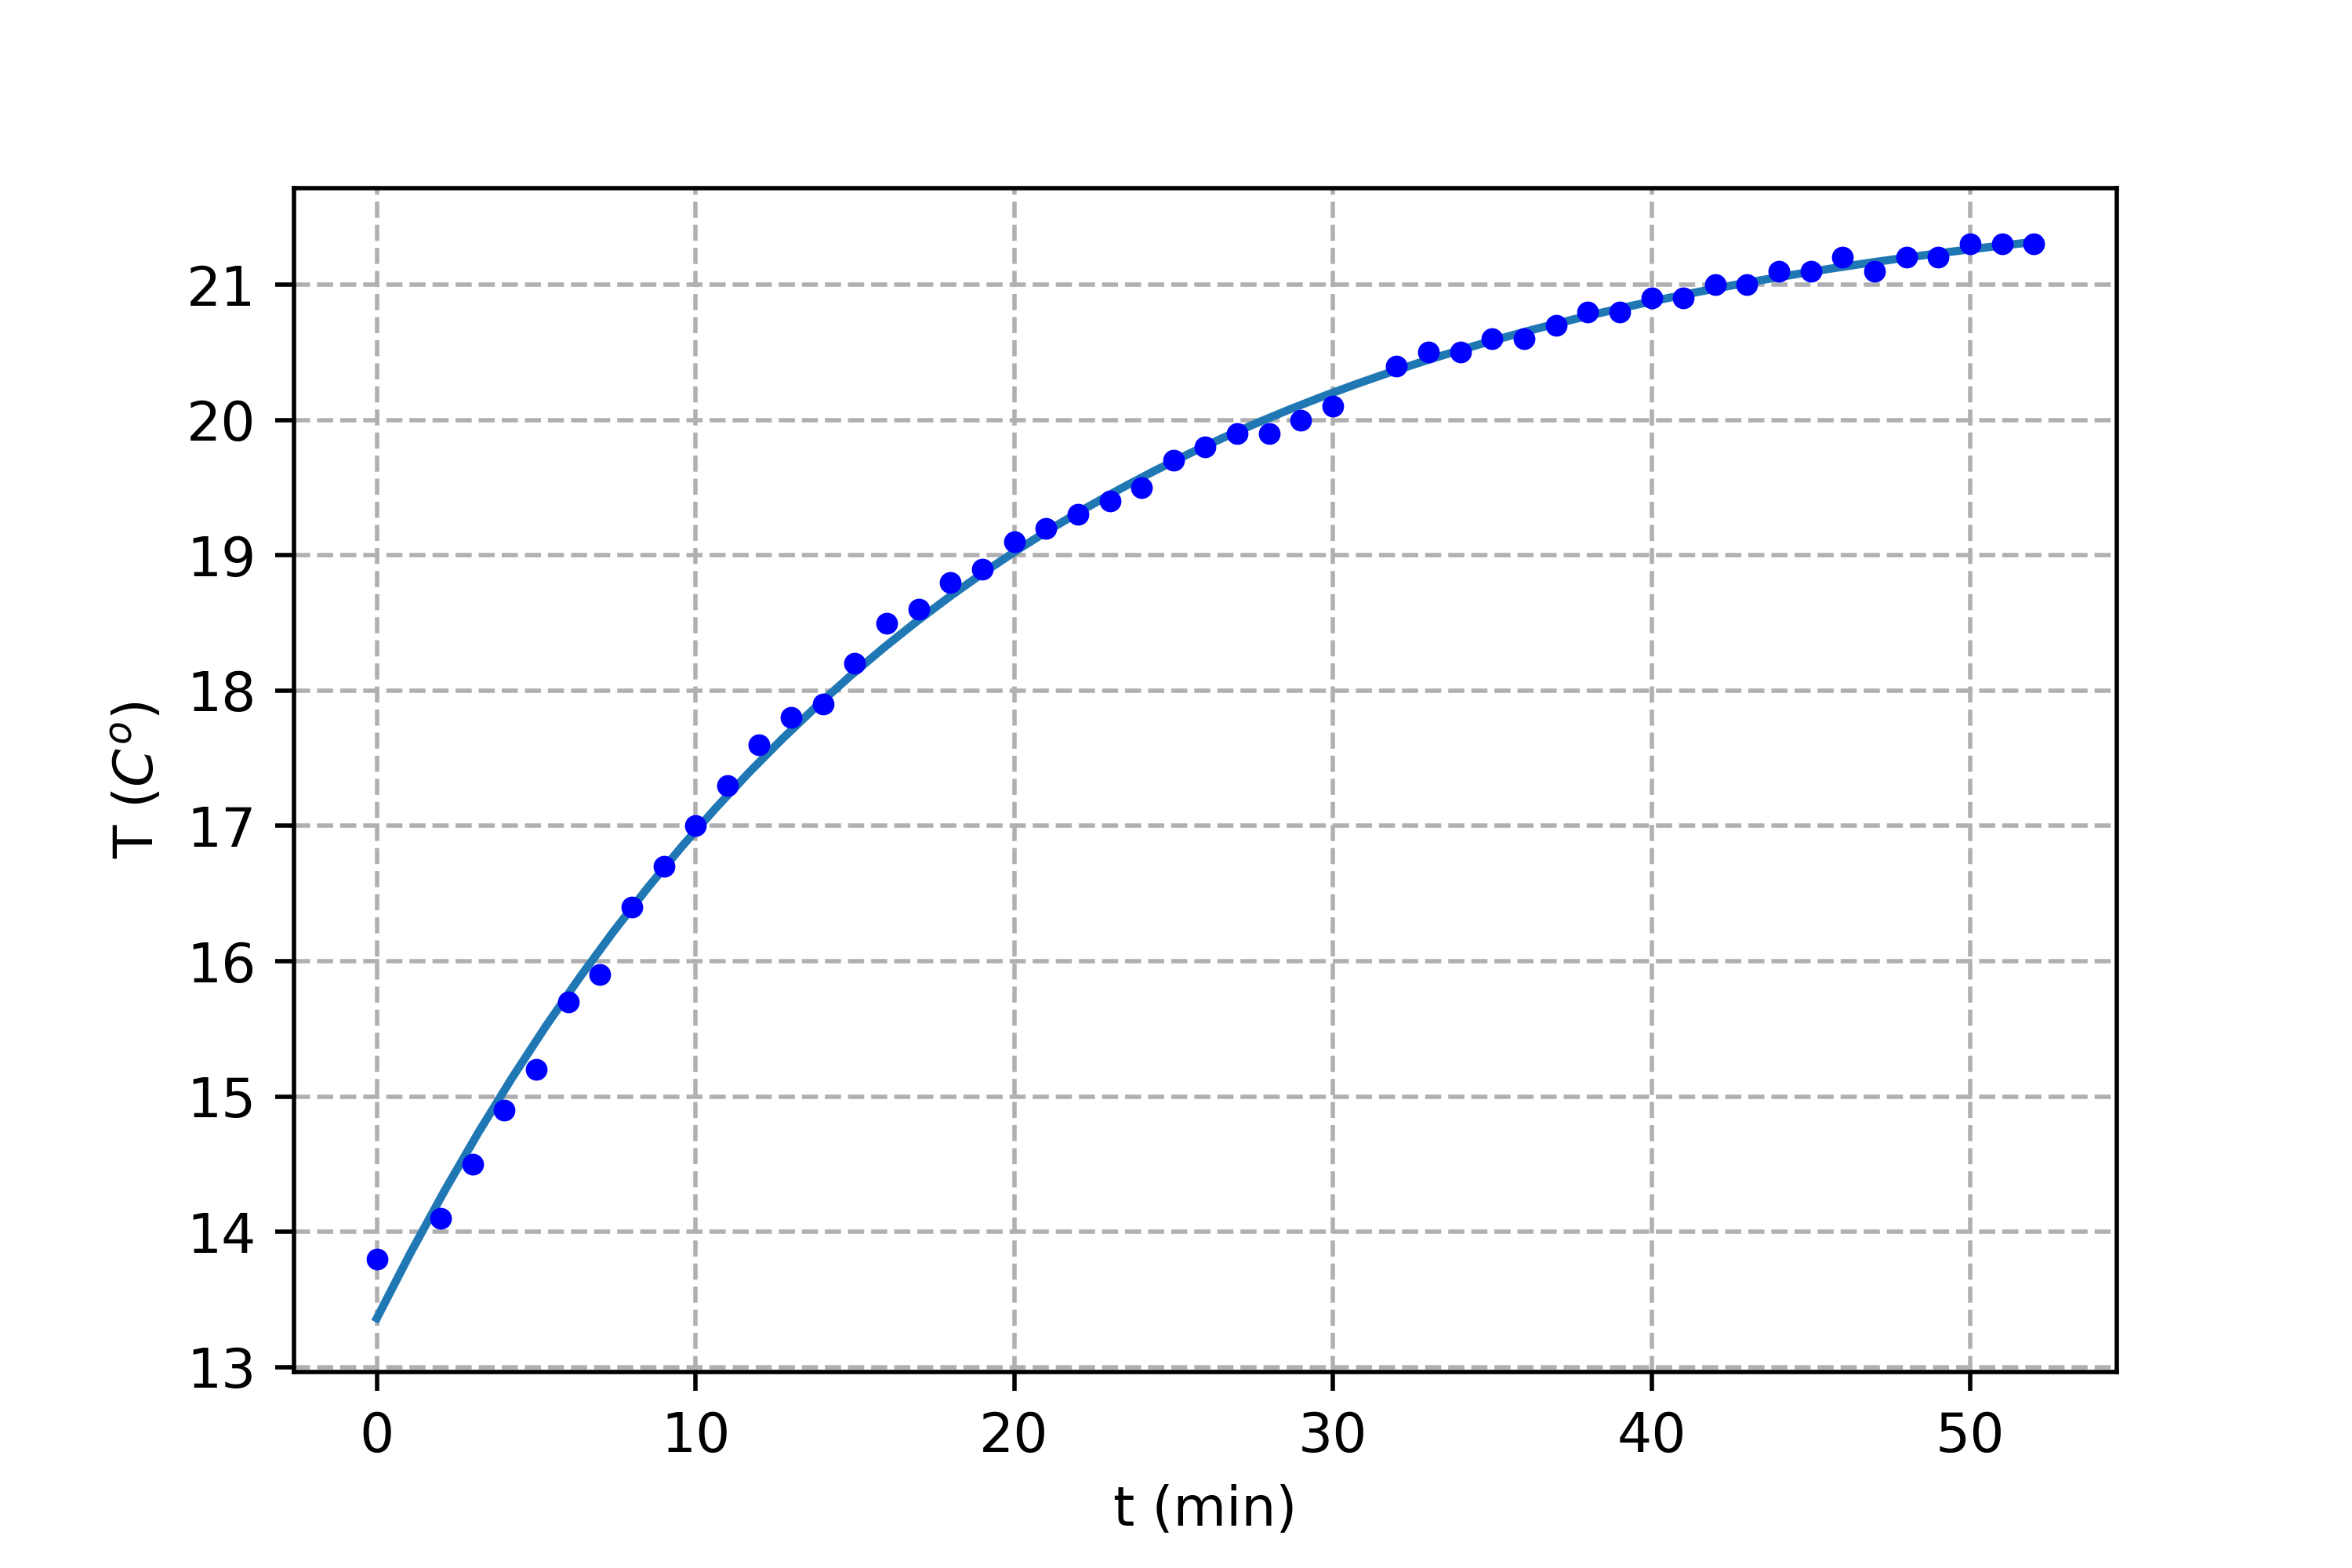
\includegraphics[scale=1.0]{plot-peltier0.png} 
\caption{representación de $T_2$ frente a $t$ para $V_0 = 120 V$ e $I = 0.525 A$} 
\label{Fig:graficapeltier1}
\end{figure}

\begin{figure}[h!] 	 \centering 
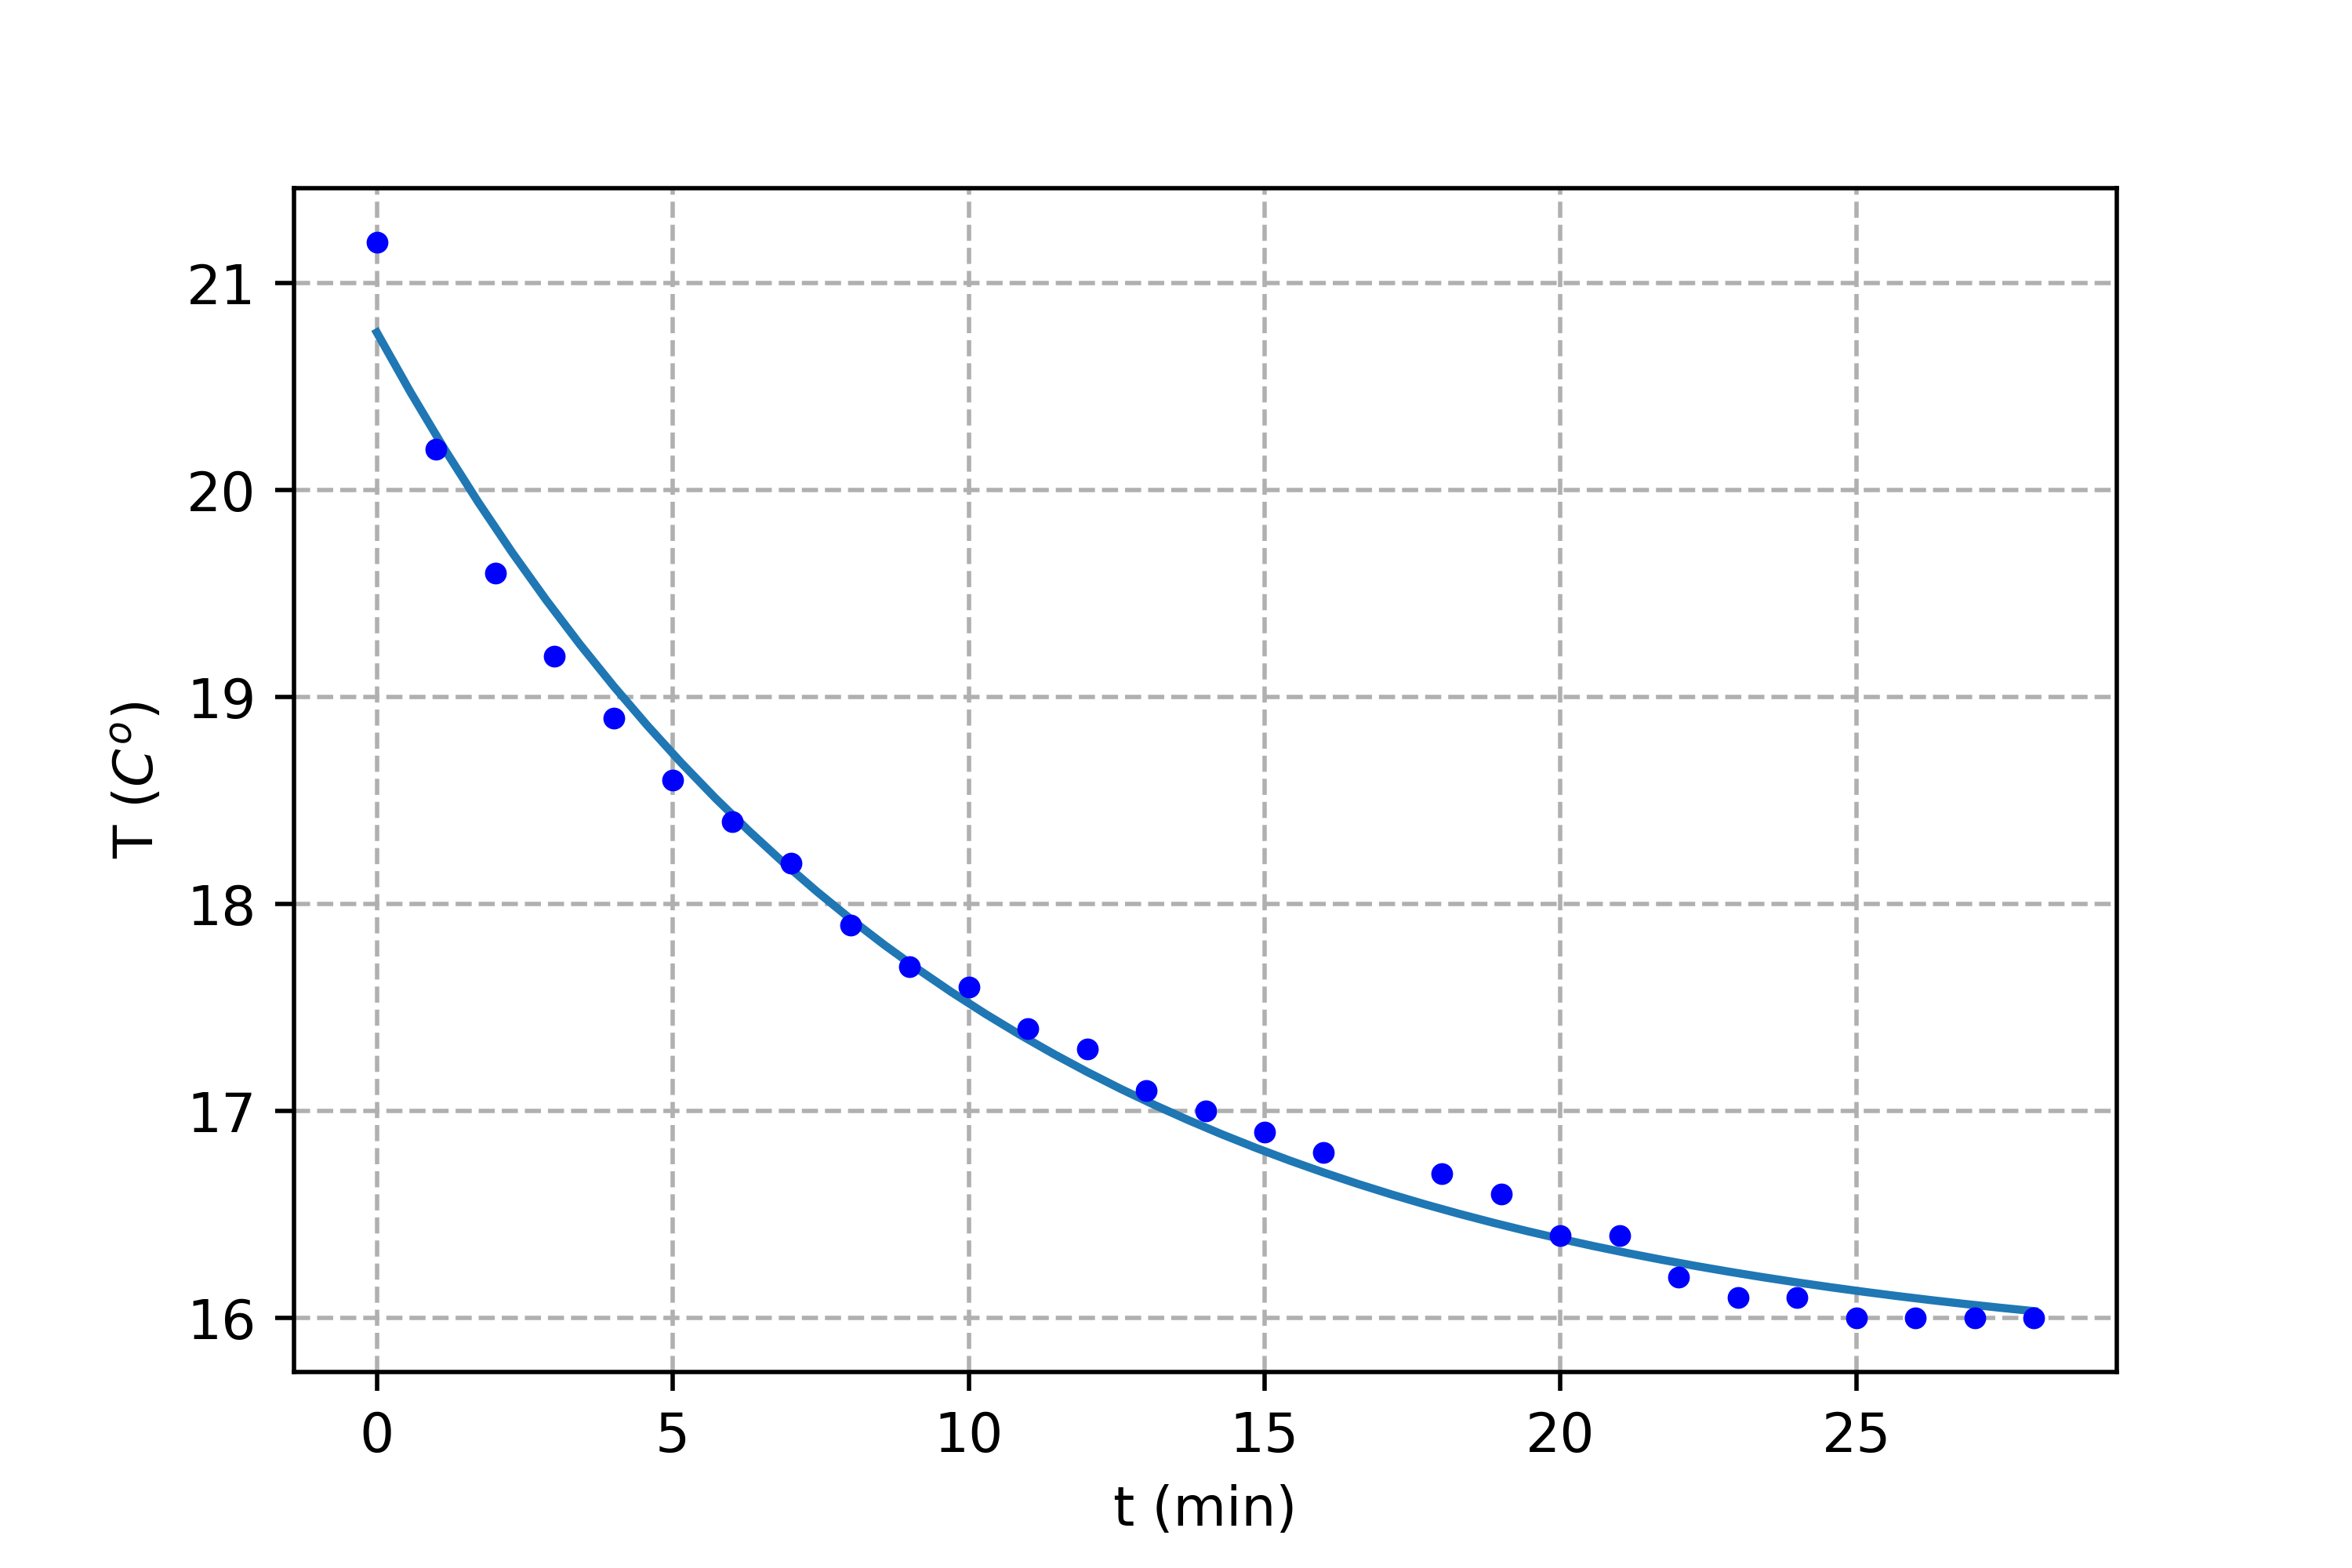
\includegraphics[scale=1.0]{plot-peltier1.png} 
\caption{representación de $T_2$ frente a $t$ para $V_0 = 120 V$ e $I = 1.001 A$} 
\label{Fig:graficapeltier2}
\end{figure} 

\begin{figure}[h!] 	 \centering 
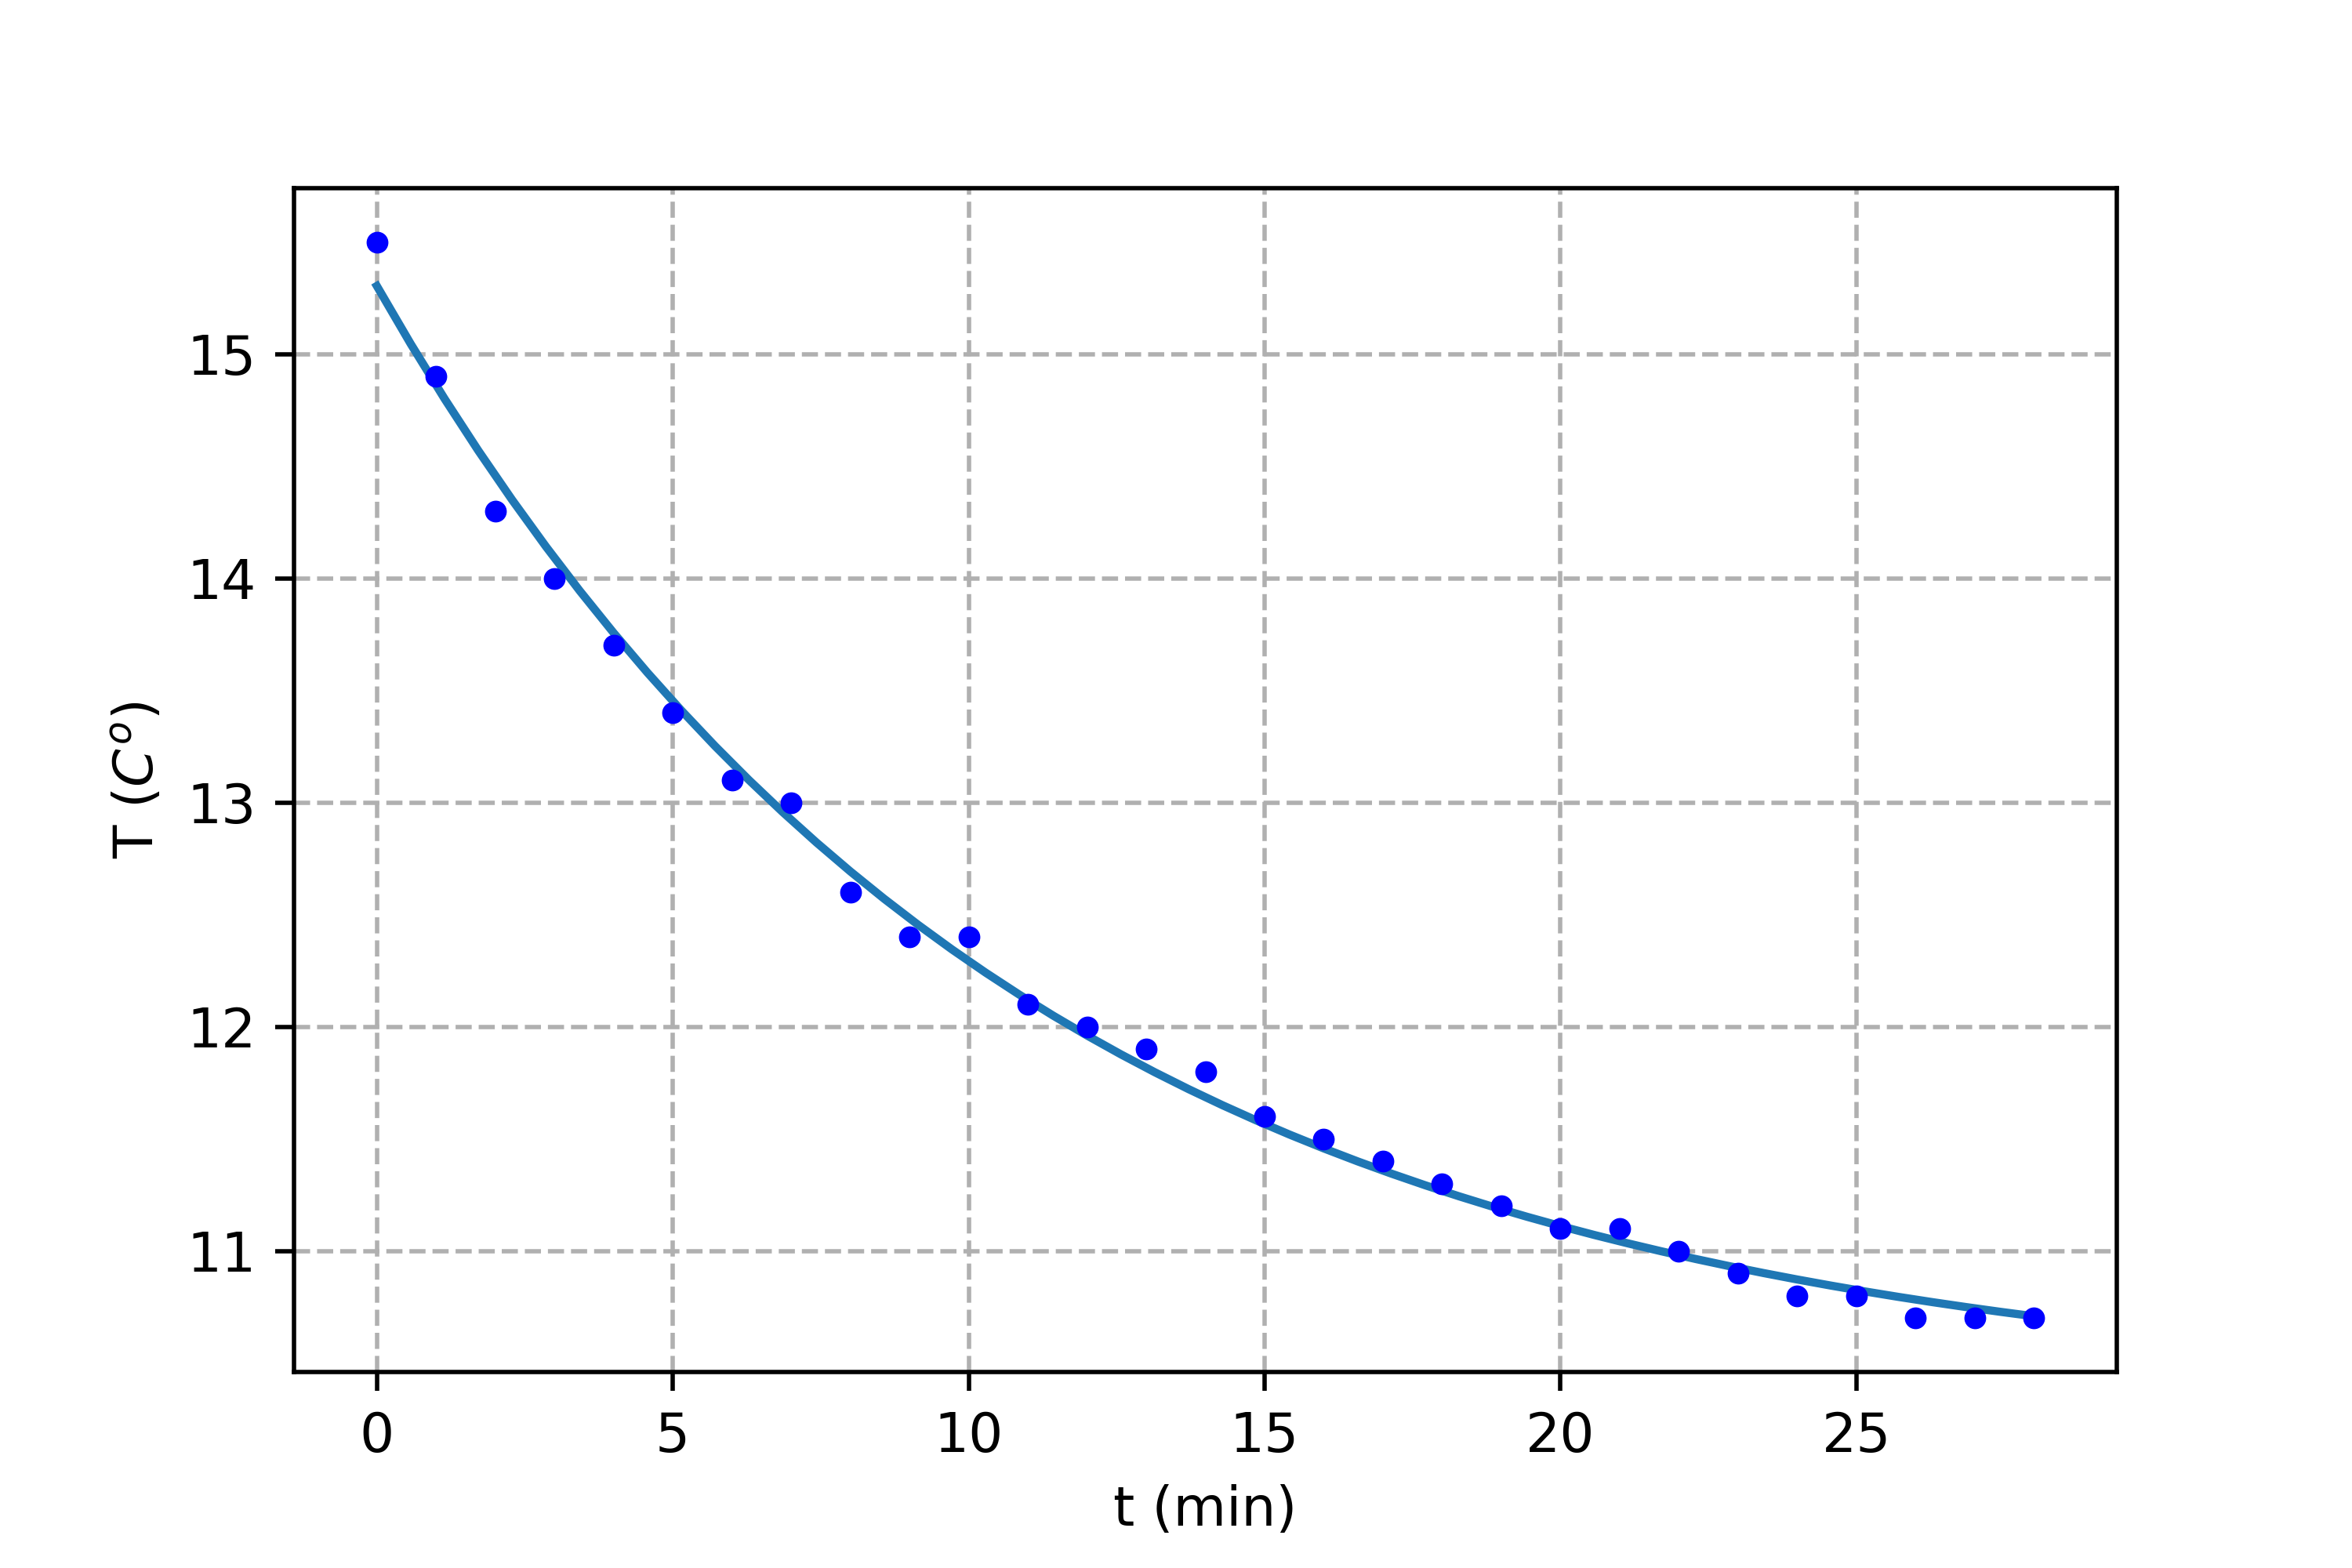
\includegraphics[scale=1.0]{plot-peltier2.png} 
\caption{representación de $T_2$ frente a $t$ para $V_0 = 120 V$ e $I = 1.522 A$} 
\label{Fig:graficapeltier3}
\end{figure} 

\begin{figure}[h!] 	 \centering 
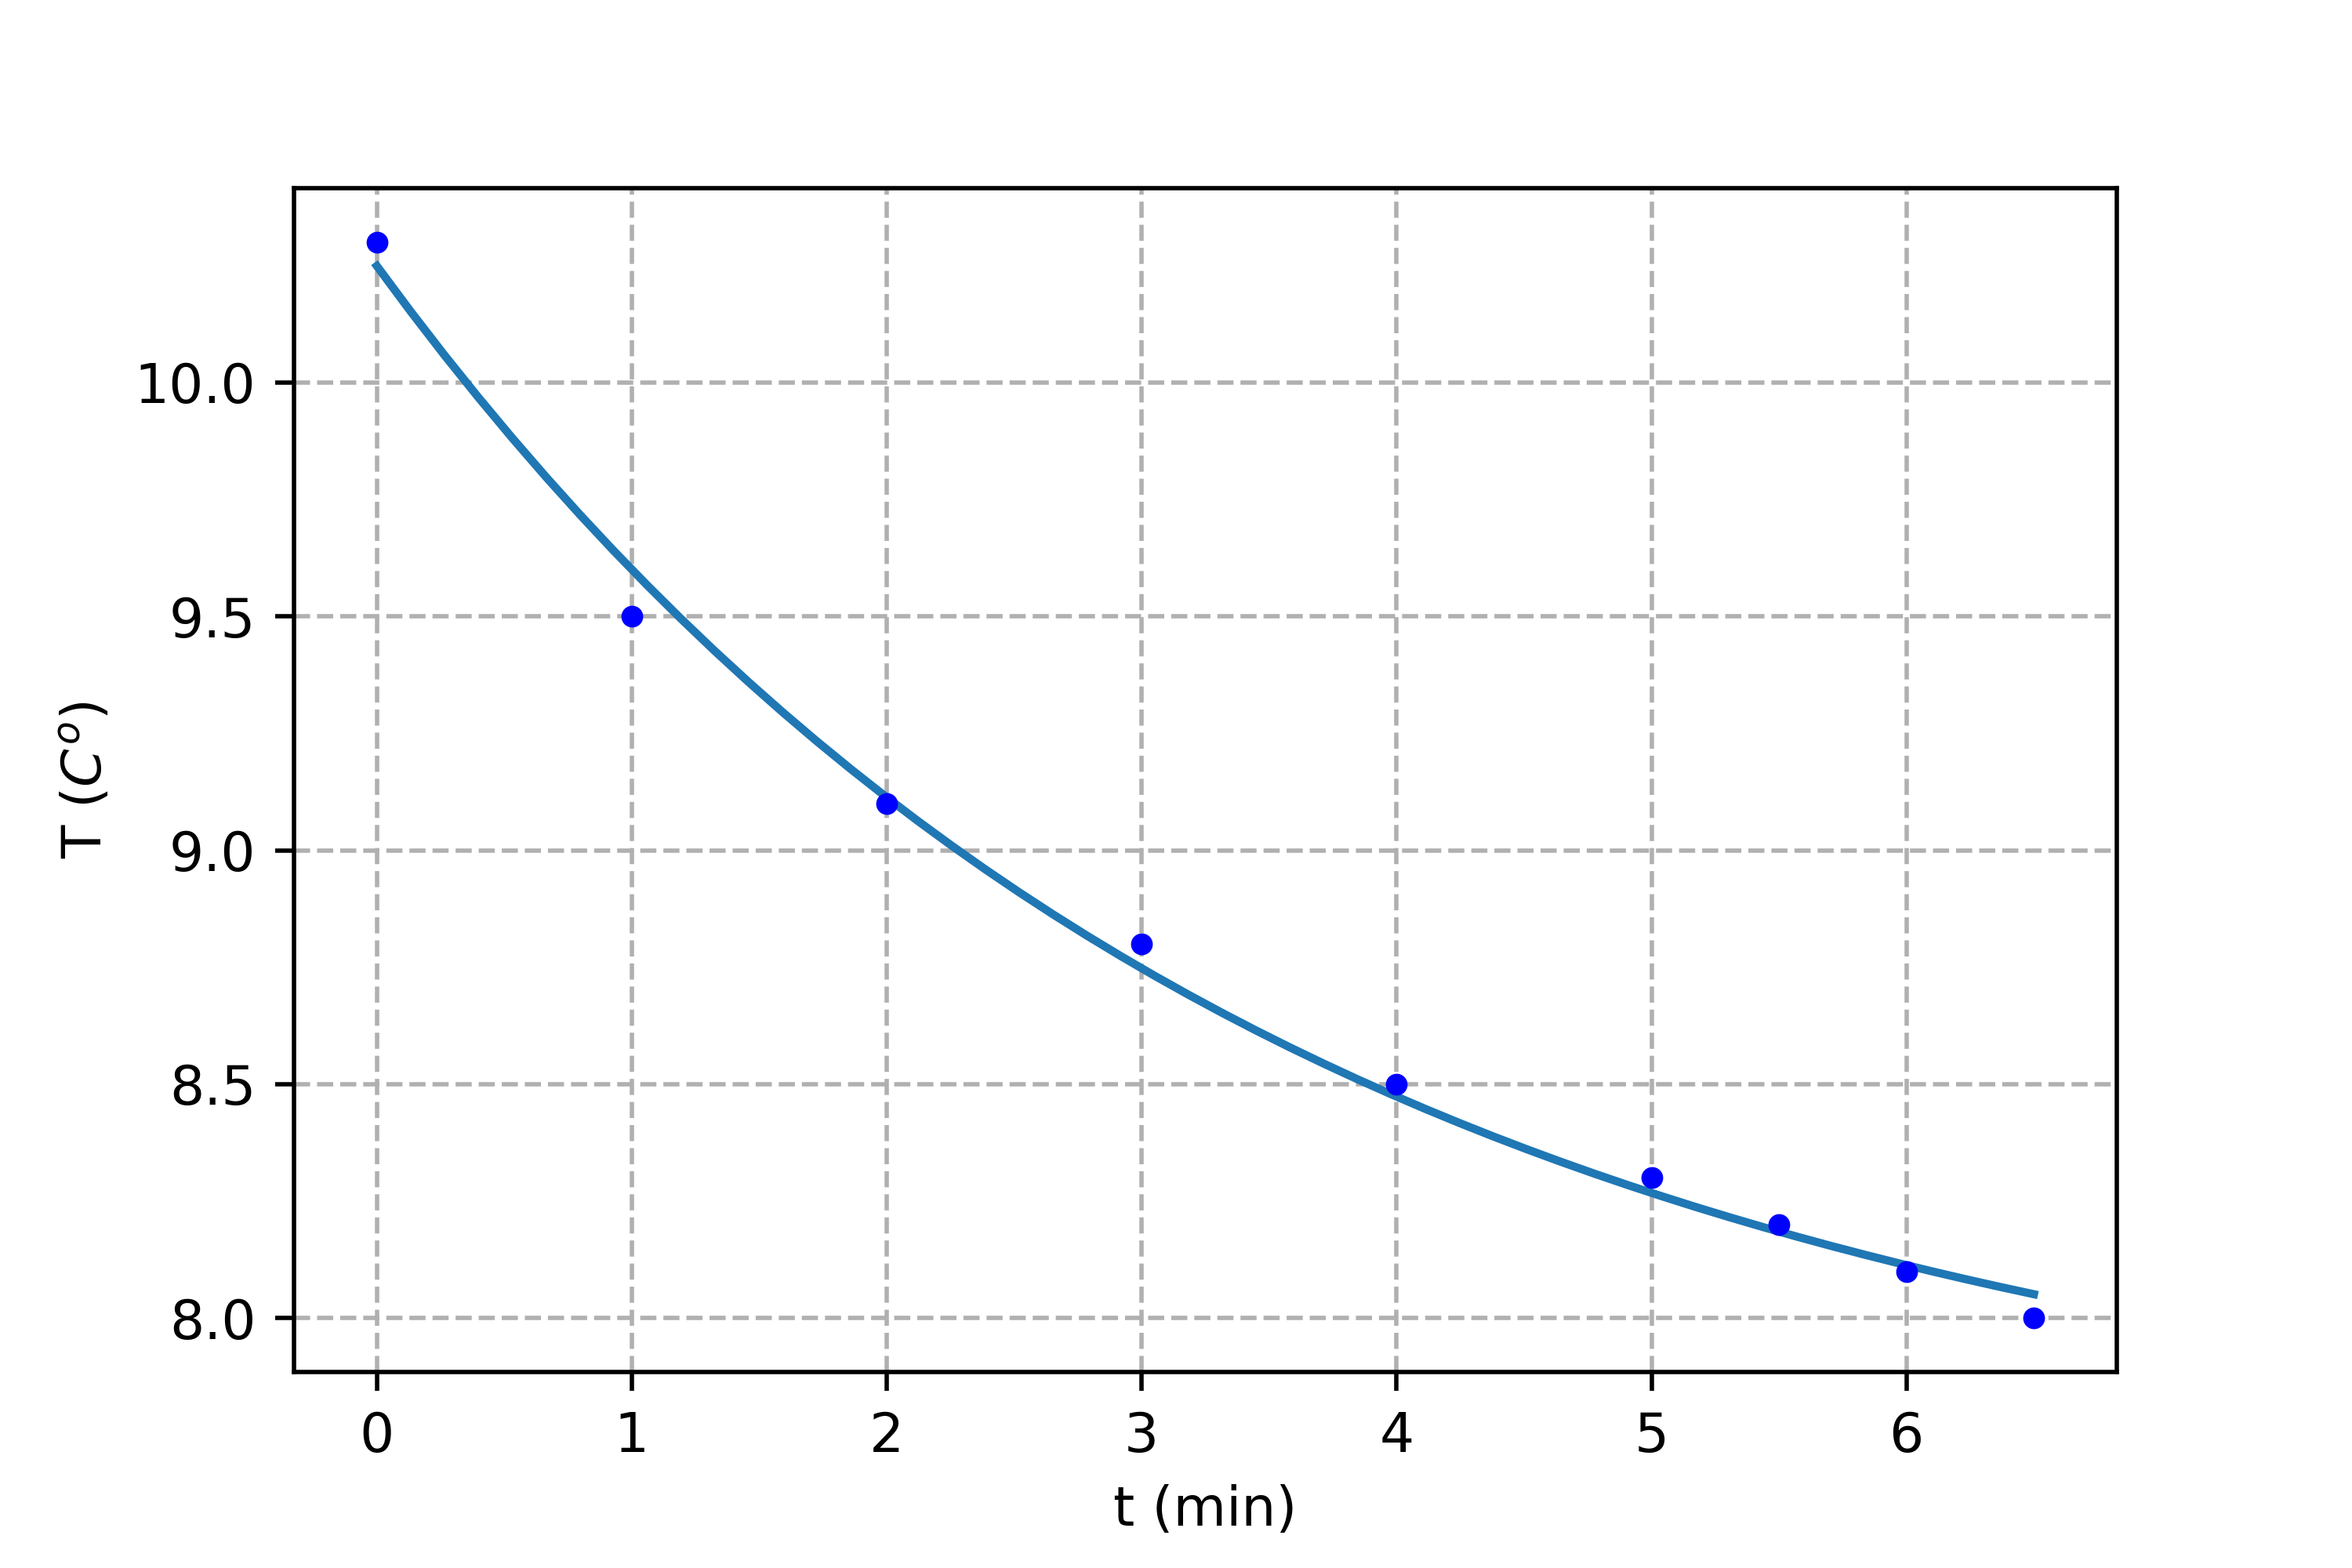
\includegraphics[scale=1.0]{plot-peltier3.png} 
\caption{representación de $T_2$ frente a $t$ para $V_0 = 120 V$ e $I = 2.000 A$} 
\label{Fig:graficapeltier4}
\end{figure} 

\begin{figure}[h!] 	 \centering 
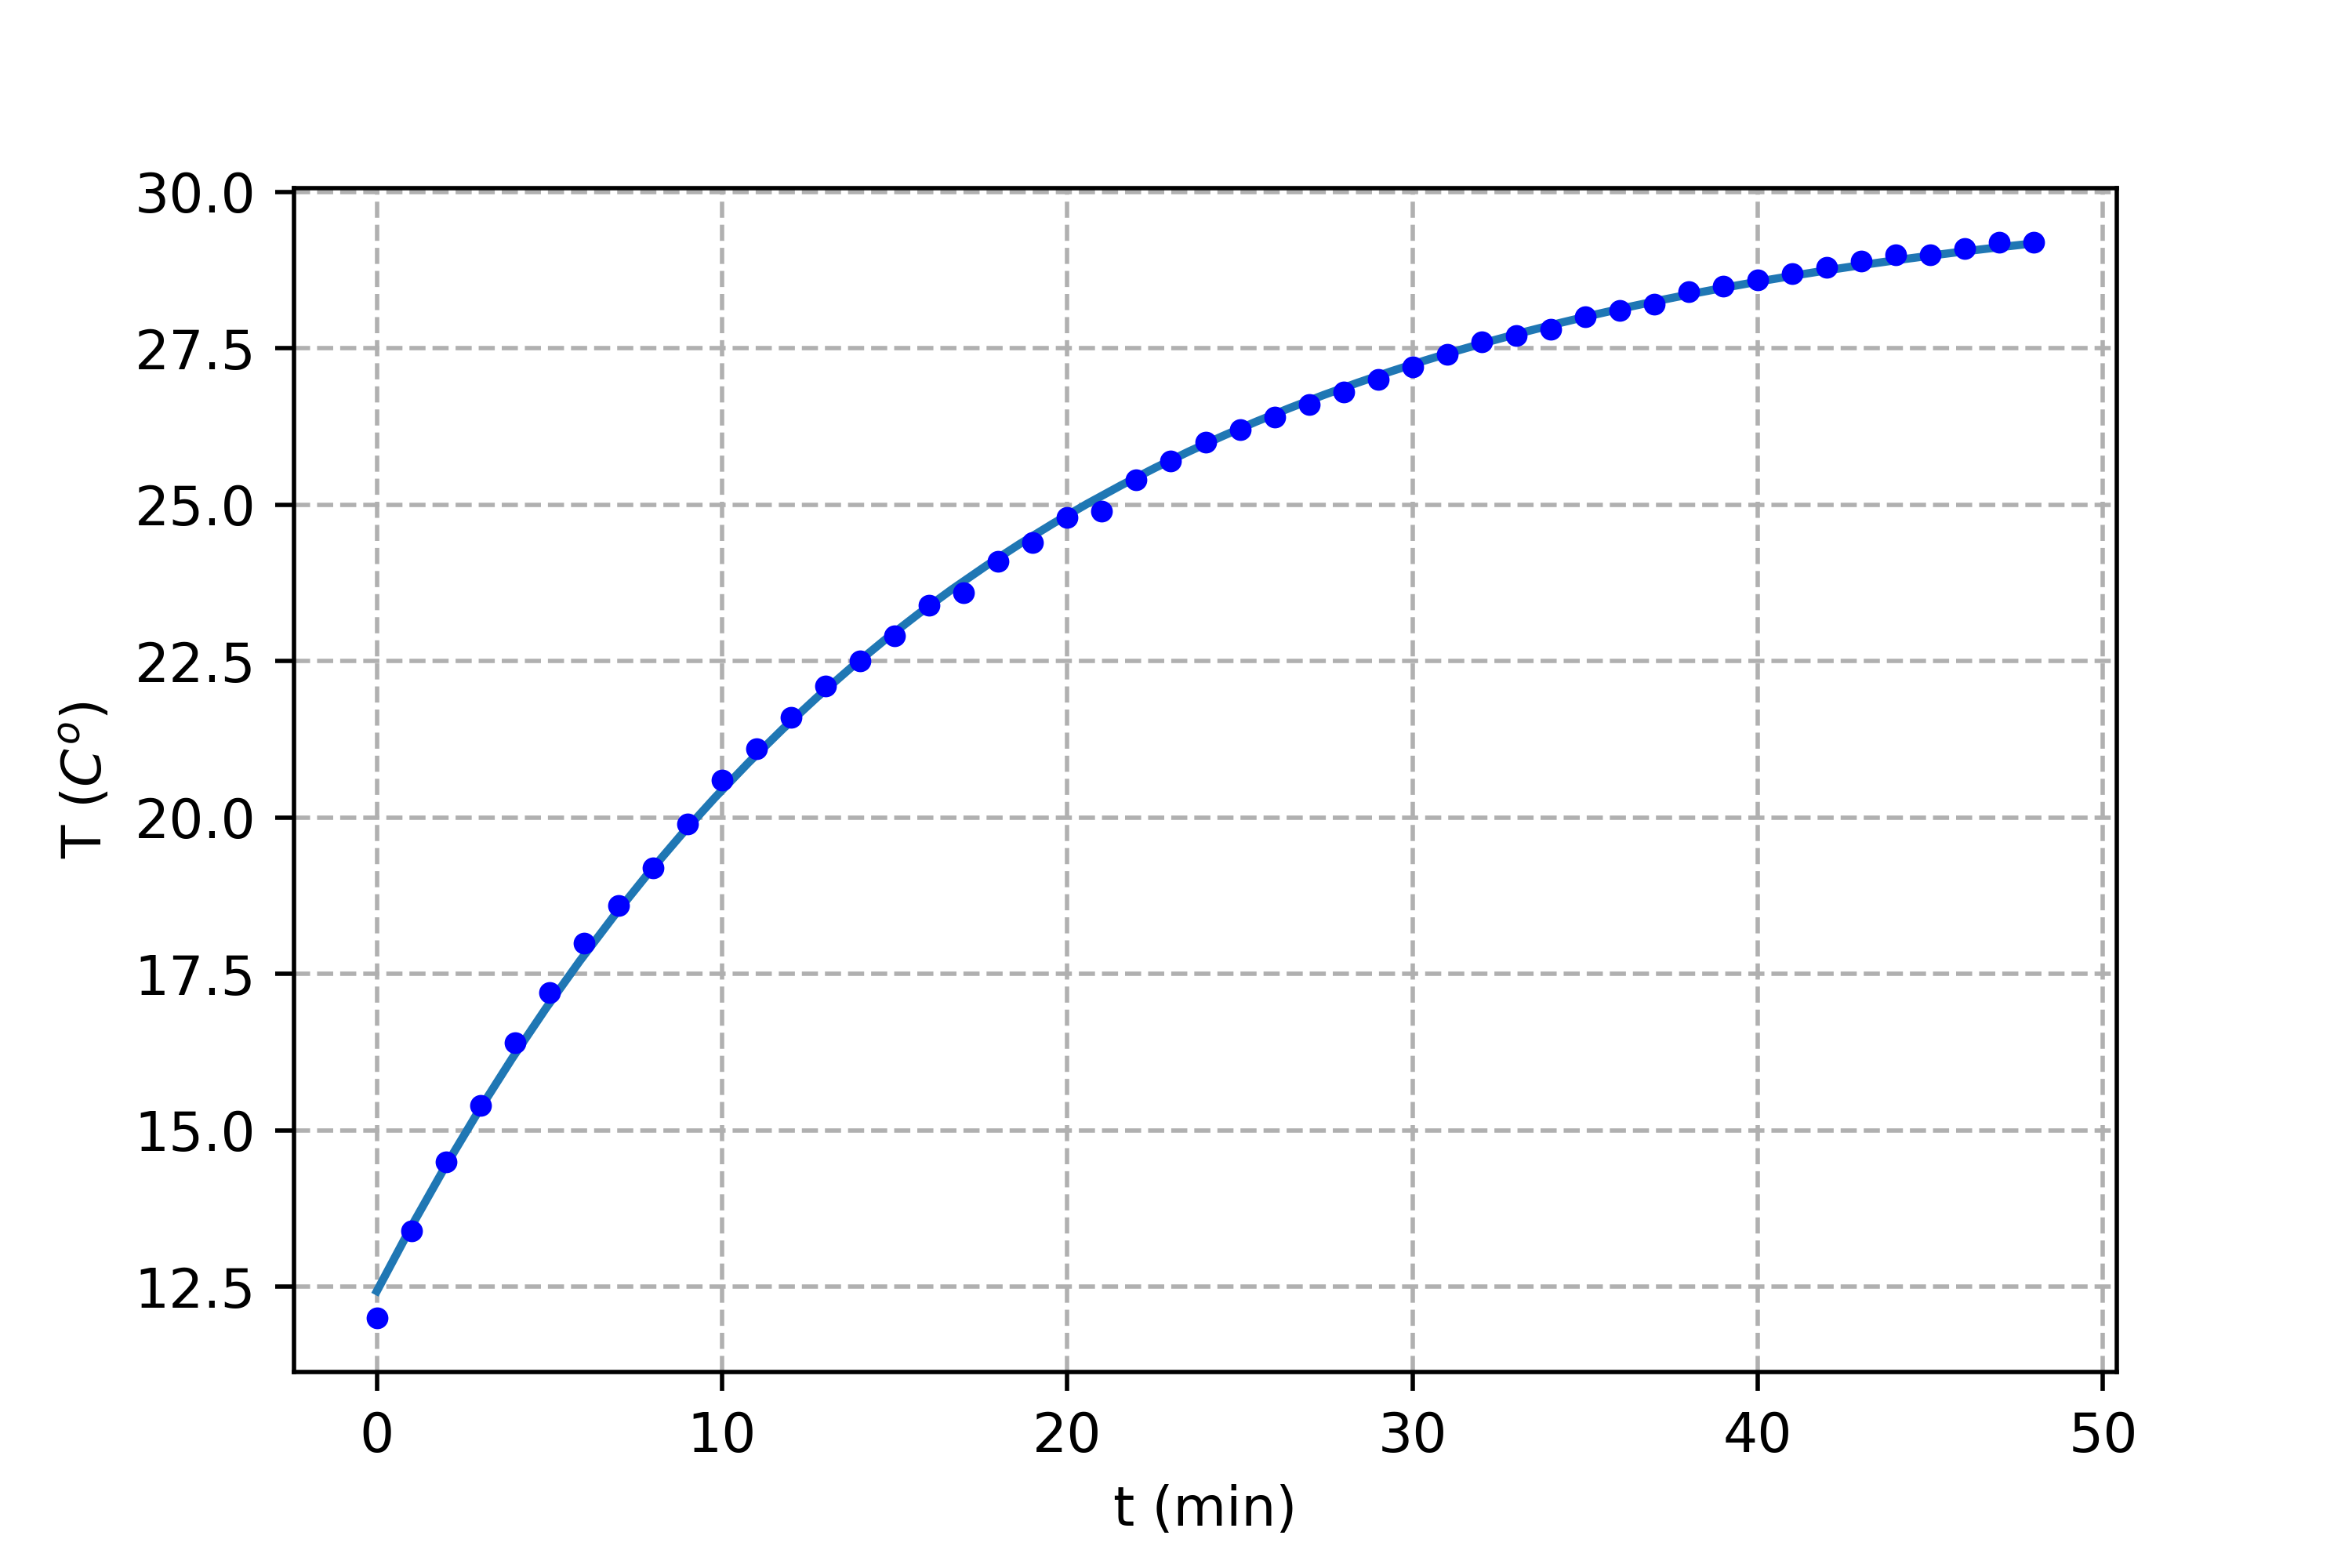
\includegraphics[scale=1.0]{plot-peltier4.png} 
\caption{representación de $T_2$ frente a $t$ para $V_0 = 150 V$ e $I = 0.512 A$} 
\label{Fig:graficapeltier5}
\end{figure} 

\begin{figure}[h!] 	 \centering 
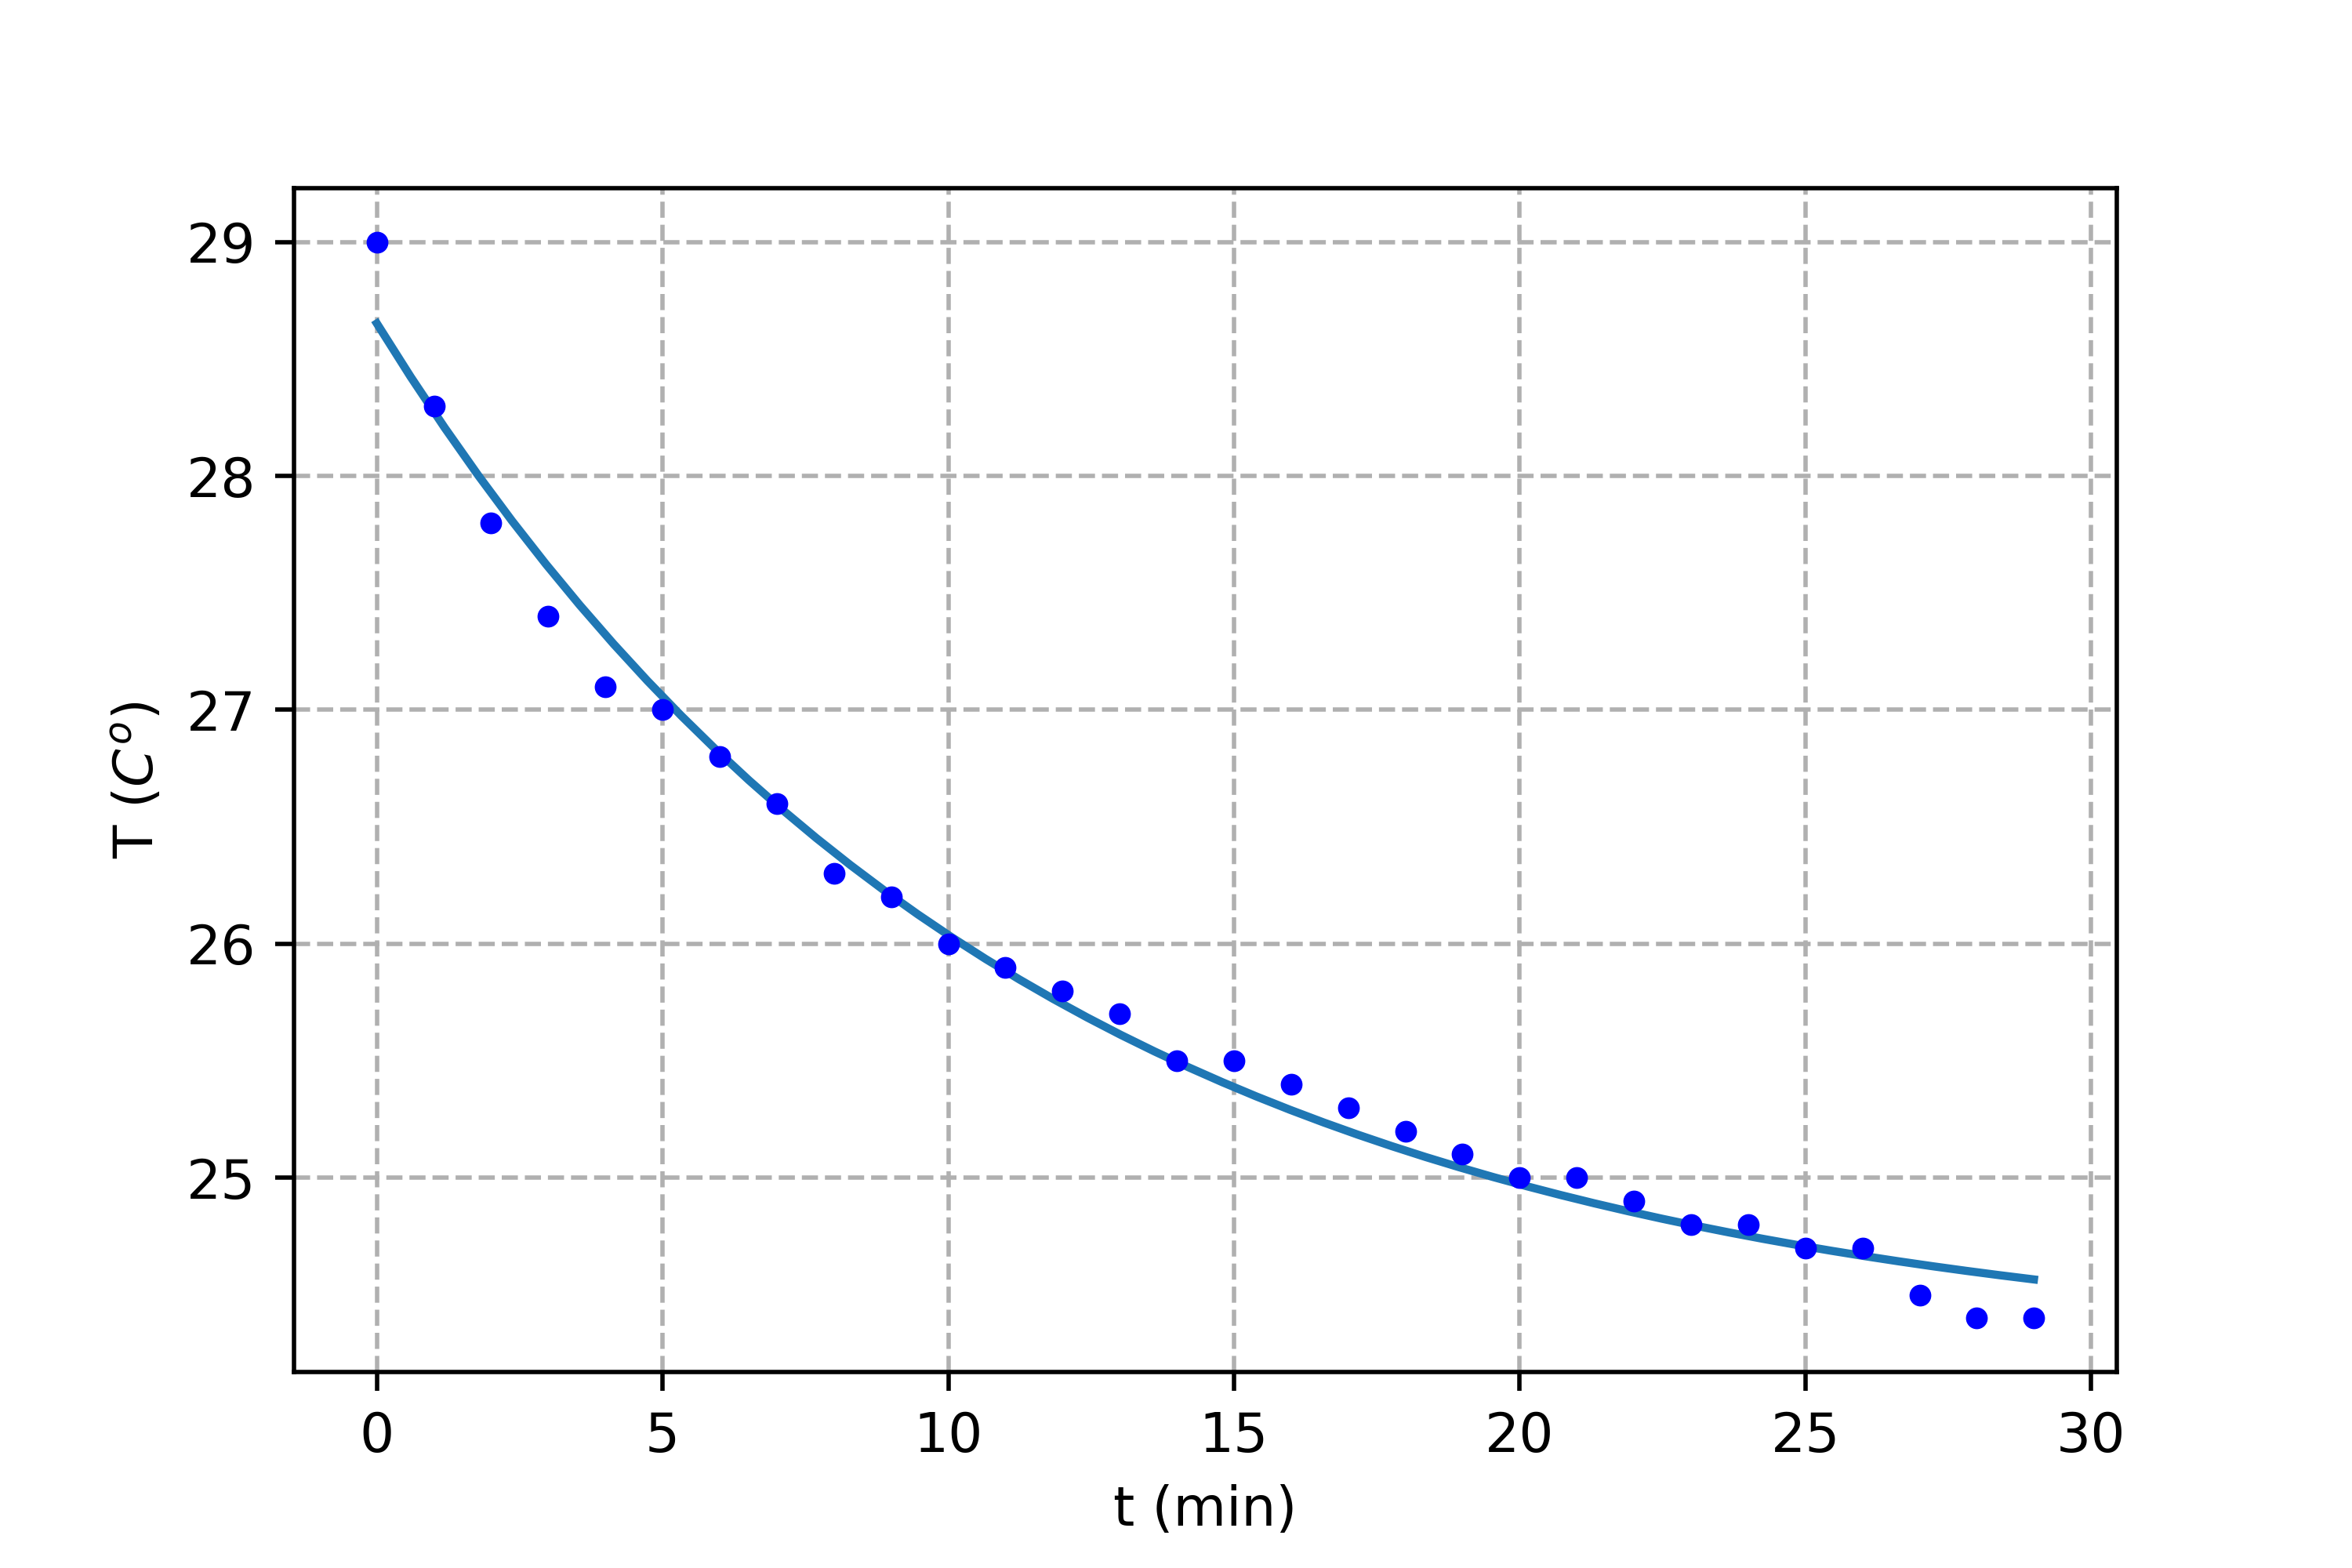
\includegraphics[scale=1.0]{plot-peltier5.png} 
\caption{representación de $T_2$ frente a $t$ para $V_0 = 150 V$ e $I = 1.013 A$} 
\label{Fig:graficapeltier6}
\end{figure} 

\begin{figure}[h!] 	 \centering 
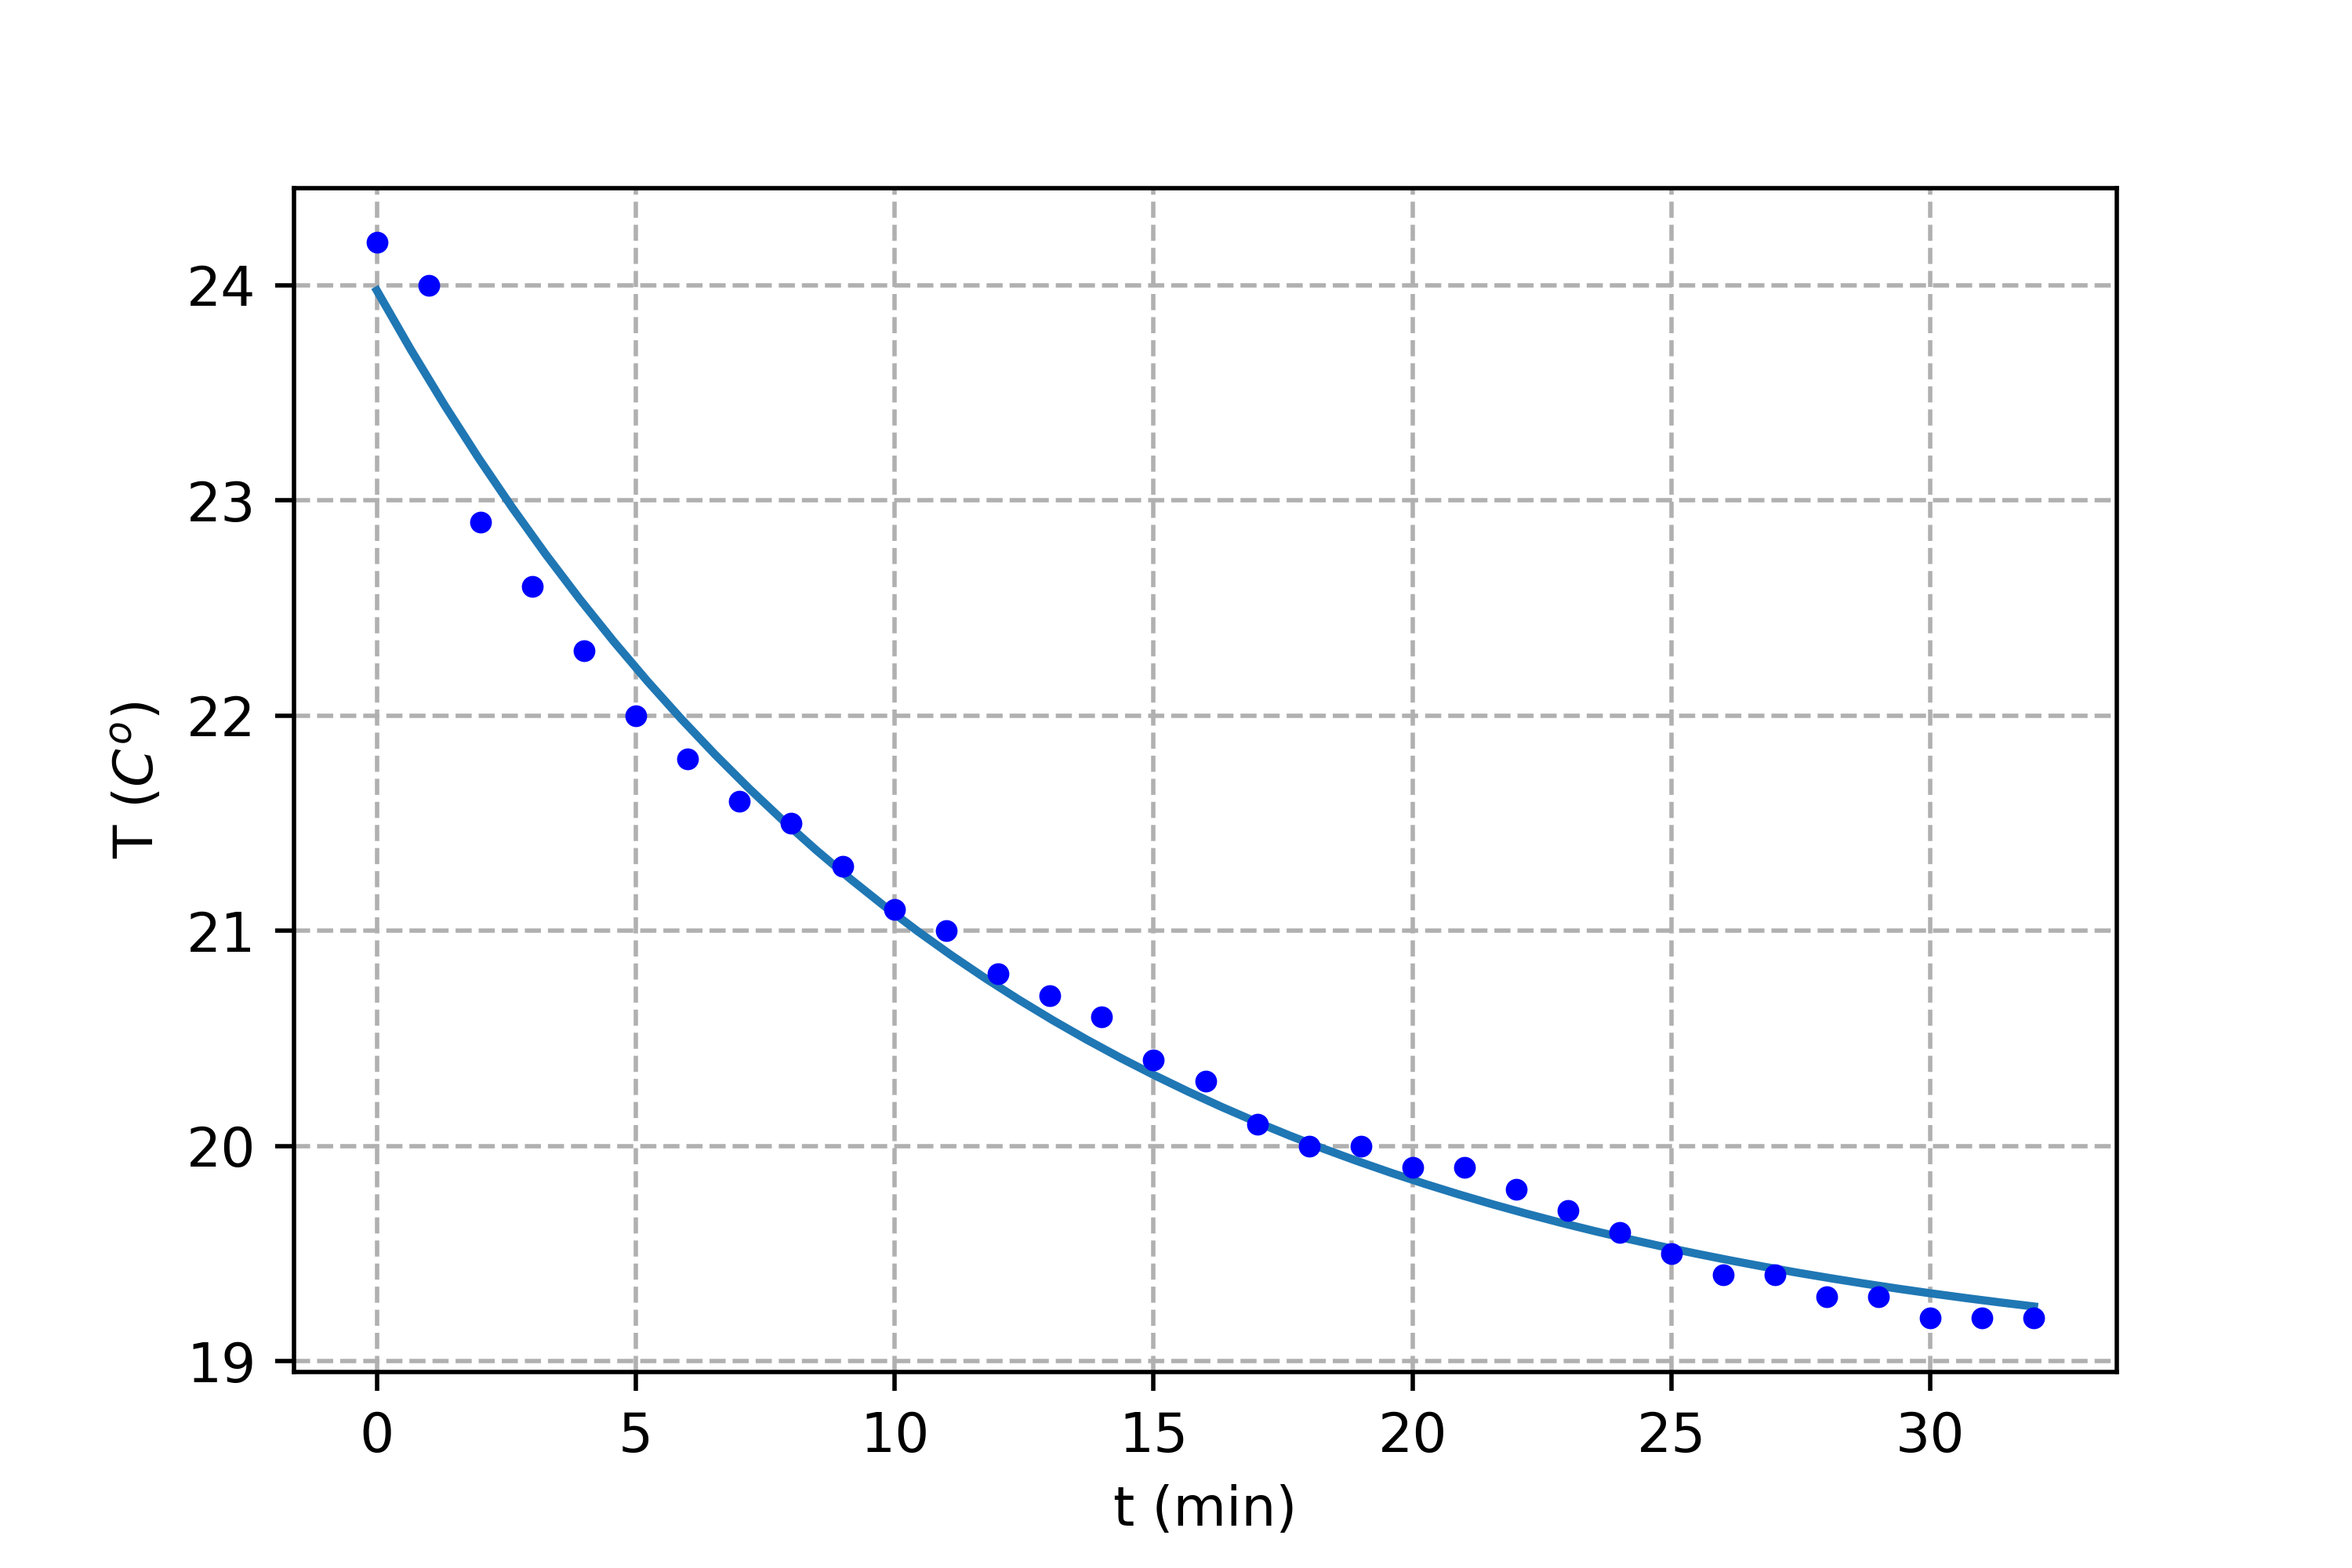
\includegraphics[scale=1]{plot-peltier6.png} 
\caption{representación de $T_2$ frente a $t$ para $V_0 = 150 V$ e $I = 1.490 A$} 
\label{Fig:graficapeltier7}
\end{figure} 



\begin{figure}[h!] 	 \centering 
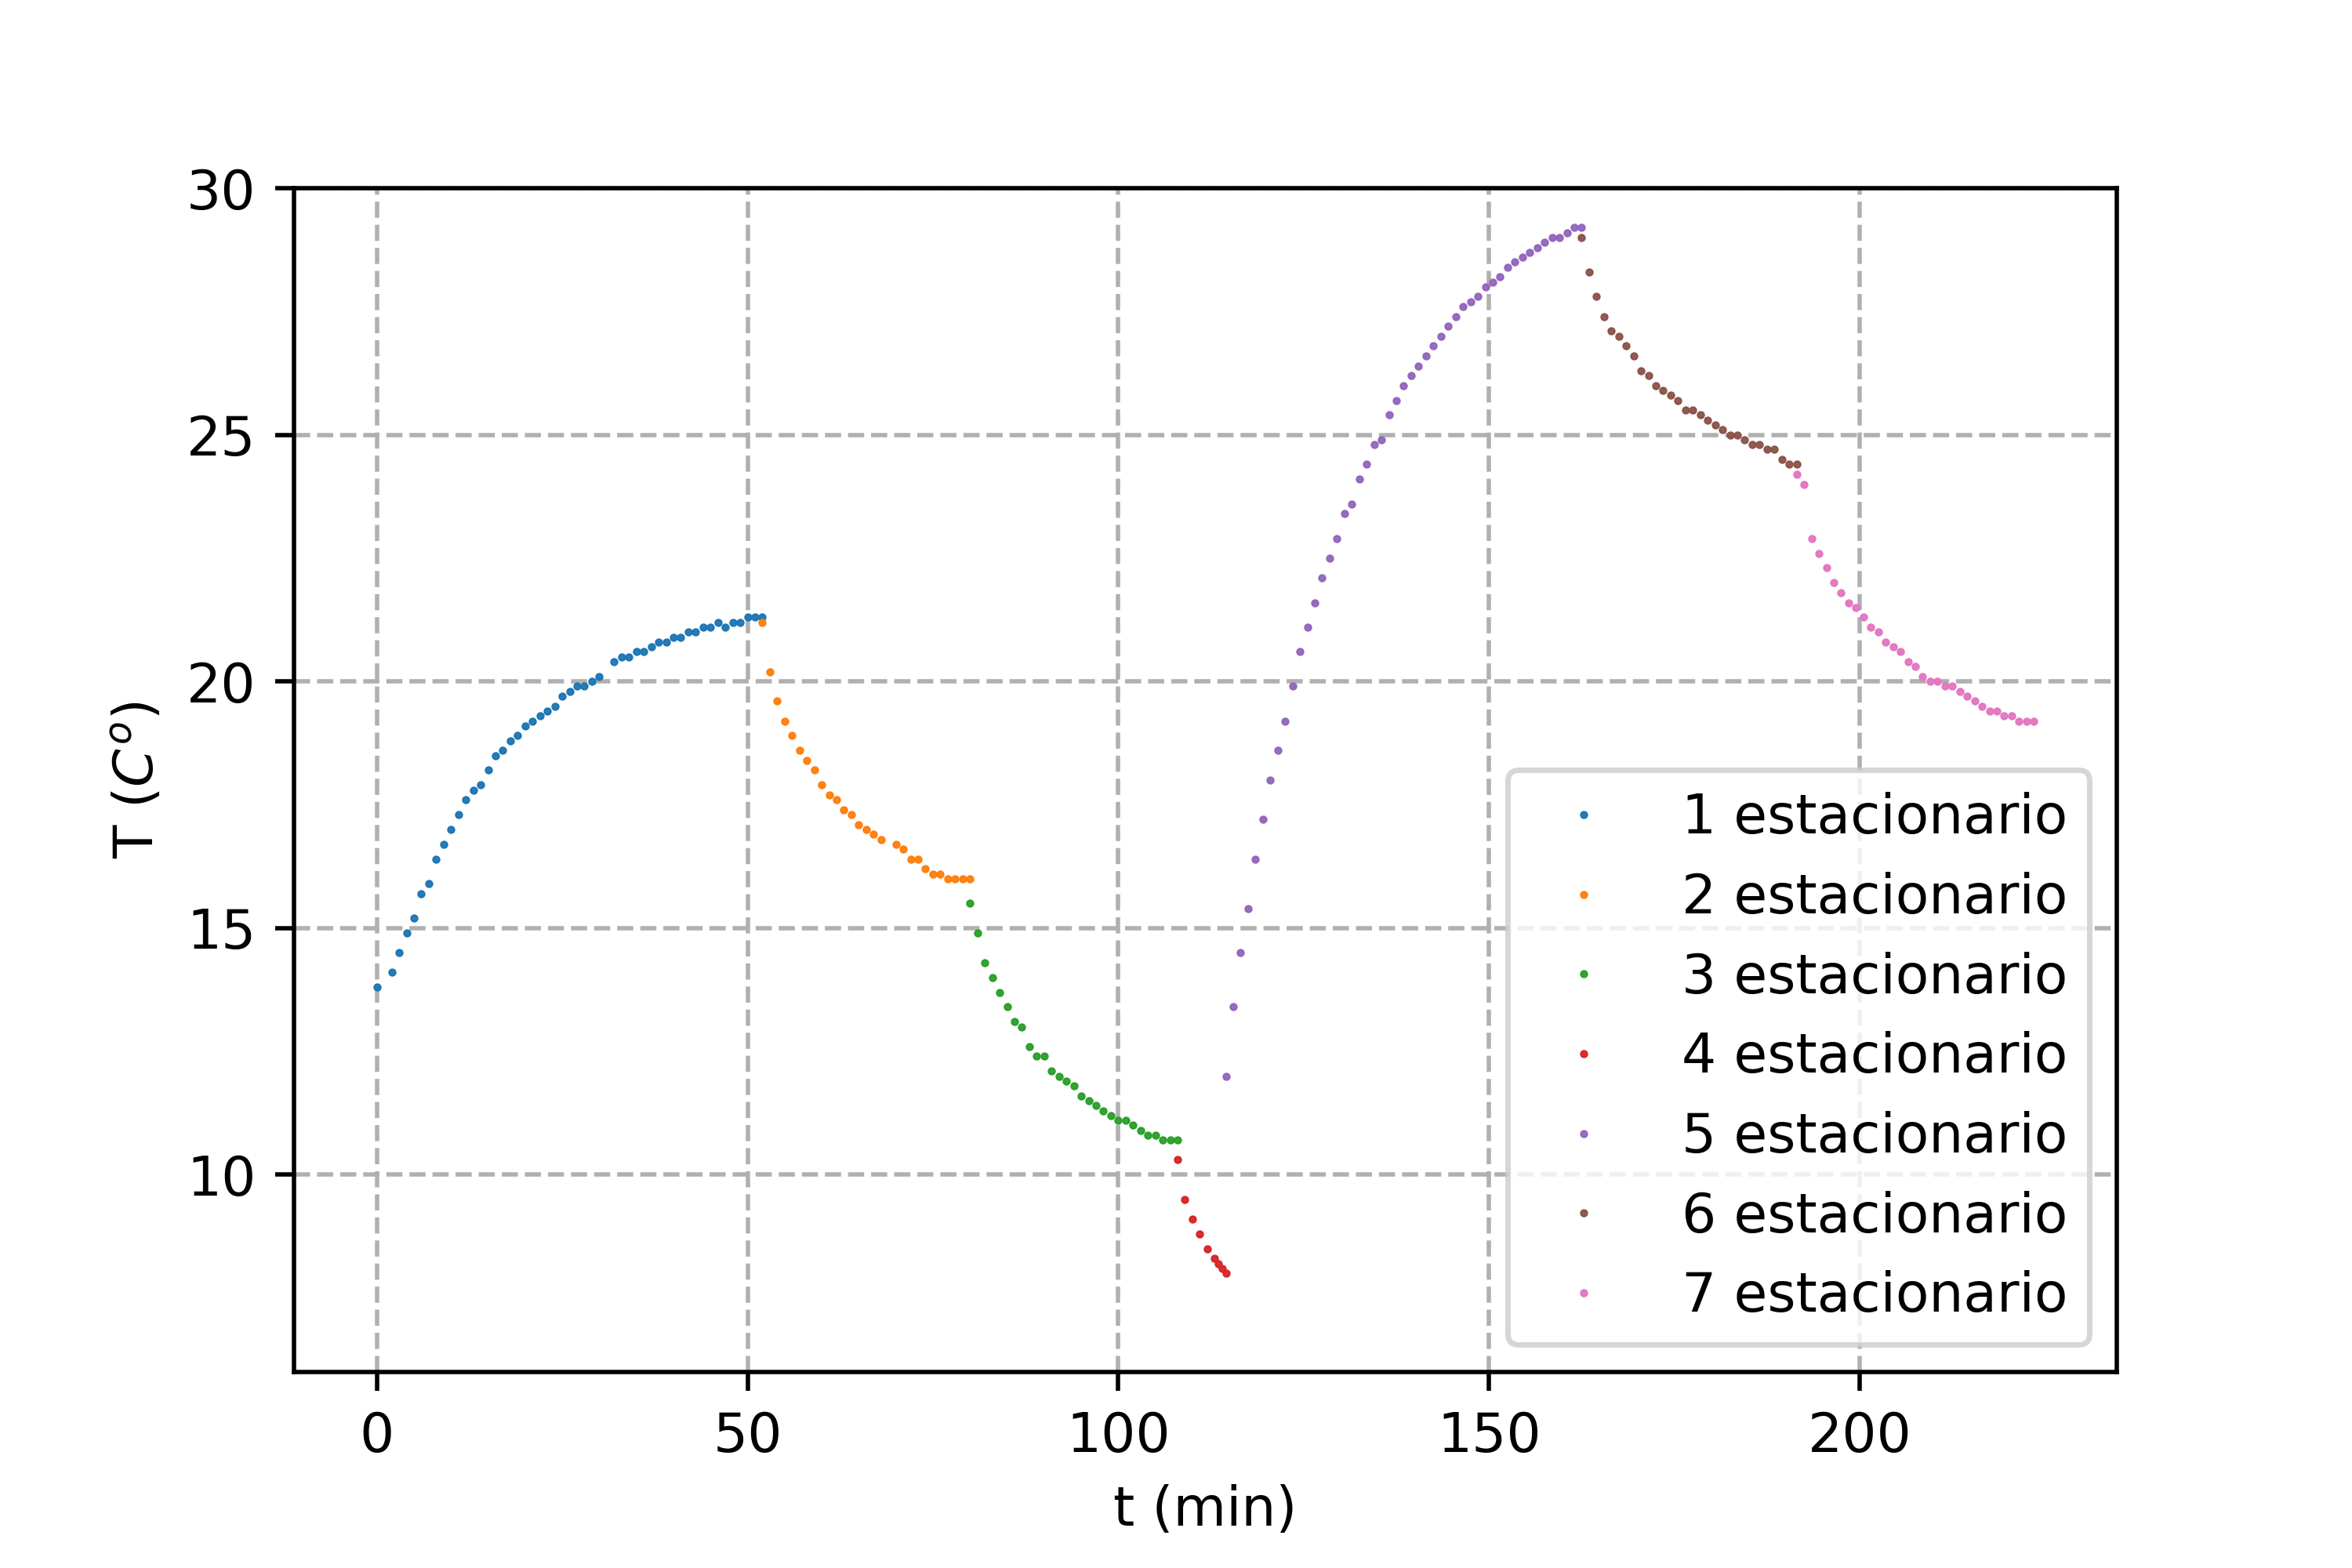
\includegraphics[scale=1.0]{plot-peltier-todos.png} 
\caption{representación gráfica de todos las evoluciones de la temperatura} 
\end{figure} 


\newpage

\subsection{Coeficiente Peltier}

Una vez tenemos los calores de Peltier para cada intensidad (y voltaje), podemos hacer un ajuste lineal tal que:

\begin{equation}
\dot{Q_p} = a + bI
\end{equation}

de tal manera que podemos ver claramente la paridad $\pi_{AB} = b$ usando la ecuación \ref{Ec:efectopeltier}. Por lo tanto podemos escribir las tablas de los valores de la regresión:

\begin{table}[h!] 	 \centering 
\begin{tabular}{|c|c|c|c|} 
\hline 
$a \ (J)$ & $s(a) \ (J)$ & $\pi_{AB} \ (J/A)$ & $s(\pi_{AB}) \ (J/A)$  \\ \hline 
-2.75  & 0.34 &  20.55 & 0.26 \\ 
\hline
\end{tabular} 
\caption{Valores del ajuste lineal para los pares (I,$\dot{Q}_P$) con voltaje $V_0=120V$} 
\label{tab:peltier1} 
\end{table} 

\begin{table}[h!] 	 \centering 
\begin{tabular}{|c|c|c|c|} 
\hline 
$a \ (J)$ & $s(a) \ (J)$ & $\pi_{AB} \ (J/A)$ & $s(\pi_{AB}) \ (J/A)$  \\ \hline 
-2.43  & 0.55 &  21.09 & 0.50 \\ 
\hline
\end{tabular} 
\caption{Valores del ajuste lineal para los pares (I,$\dot{Q}_P$) con voltaje $V_0=150V$} 
\label{tab:peltier2} 
\end{table} 

\begin{table}[h!] 	 \centering 
\begin{tabular}{|c|c|} 
\hline 
$ \pi_{AB} \ (J/A)$ & $s(\pi_{AB}) \ (J/A)$  \\ \hline 
20.66 & 0.39 \\ 
\hline
\end{tabular} 
\caption{valor medio del coeficiente Peltier} 
\label{tab:20} 
\end{table} 


En este caso el valor $a$ es entendido como parte del error de la regresión lineal y la toma de datos. Como es un valor de $a$ relativamente grande, podemos asumir que la incertidumbre de $\pi_{AB}$ es mucho mayor que la que se obtiene como simple valor de la regresión lineal. Sin embargo no tenemos los suficientes conocimientos como para añadirle dicho error, ya que no sabemos como se comporta el la pendiente con cambios de $a$. Requeriría un estudio mucho mas riguroso de los datos, inclusive con una mayor toma de datos. Sin embargo como dicho tratamiento no es el objetivo de está práctica, nos limitaremos a sugerir que la incertidumbre del coeficiente será cualitativamente mayor que la que escribimos. 


\begin{figure}[h!] 	 \centering 
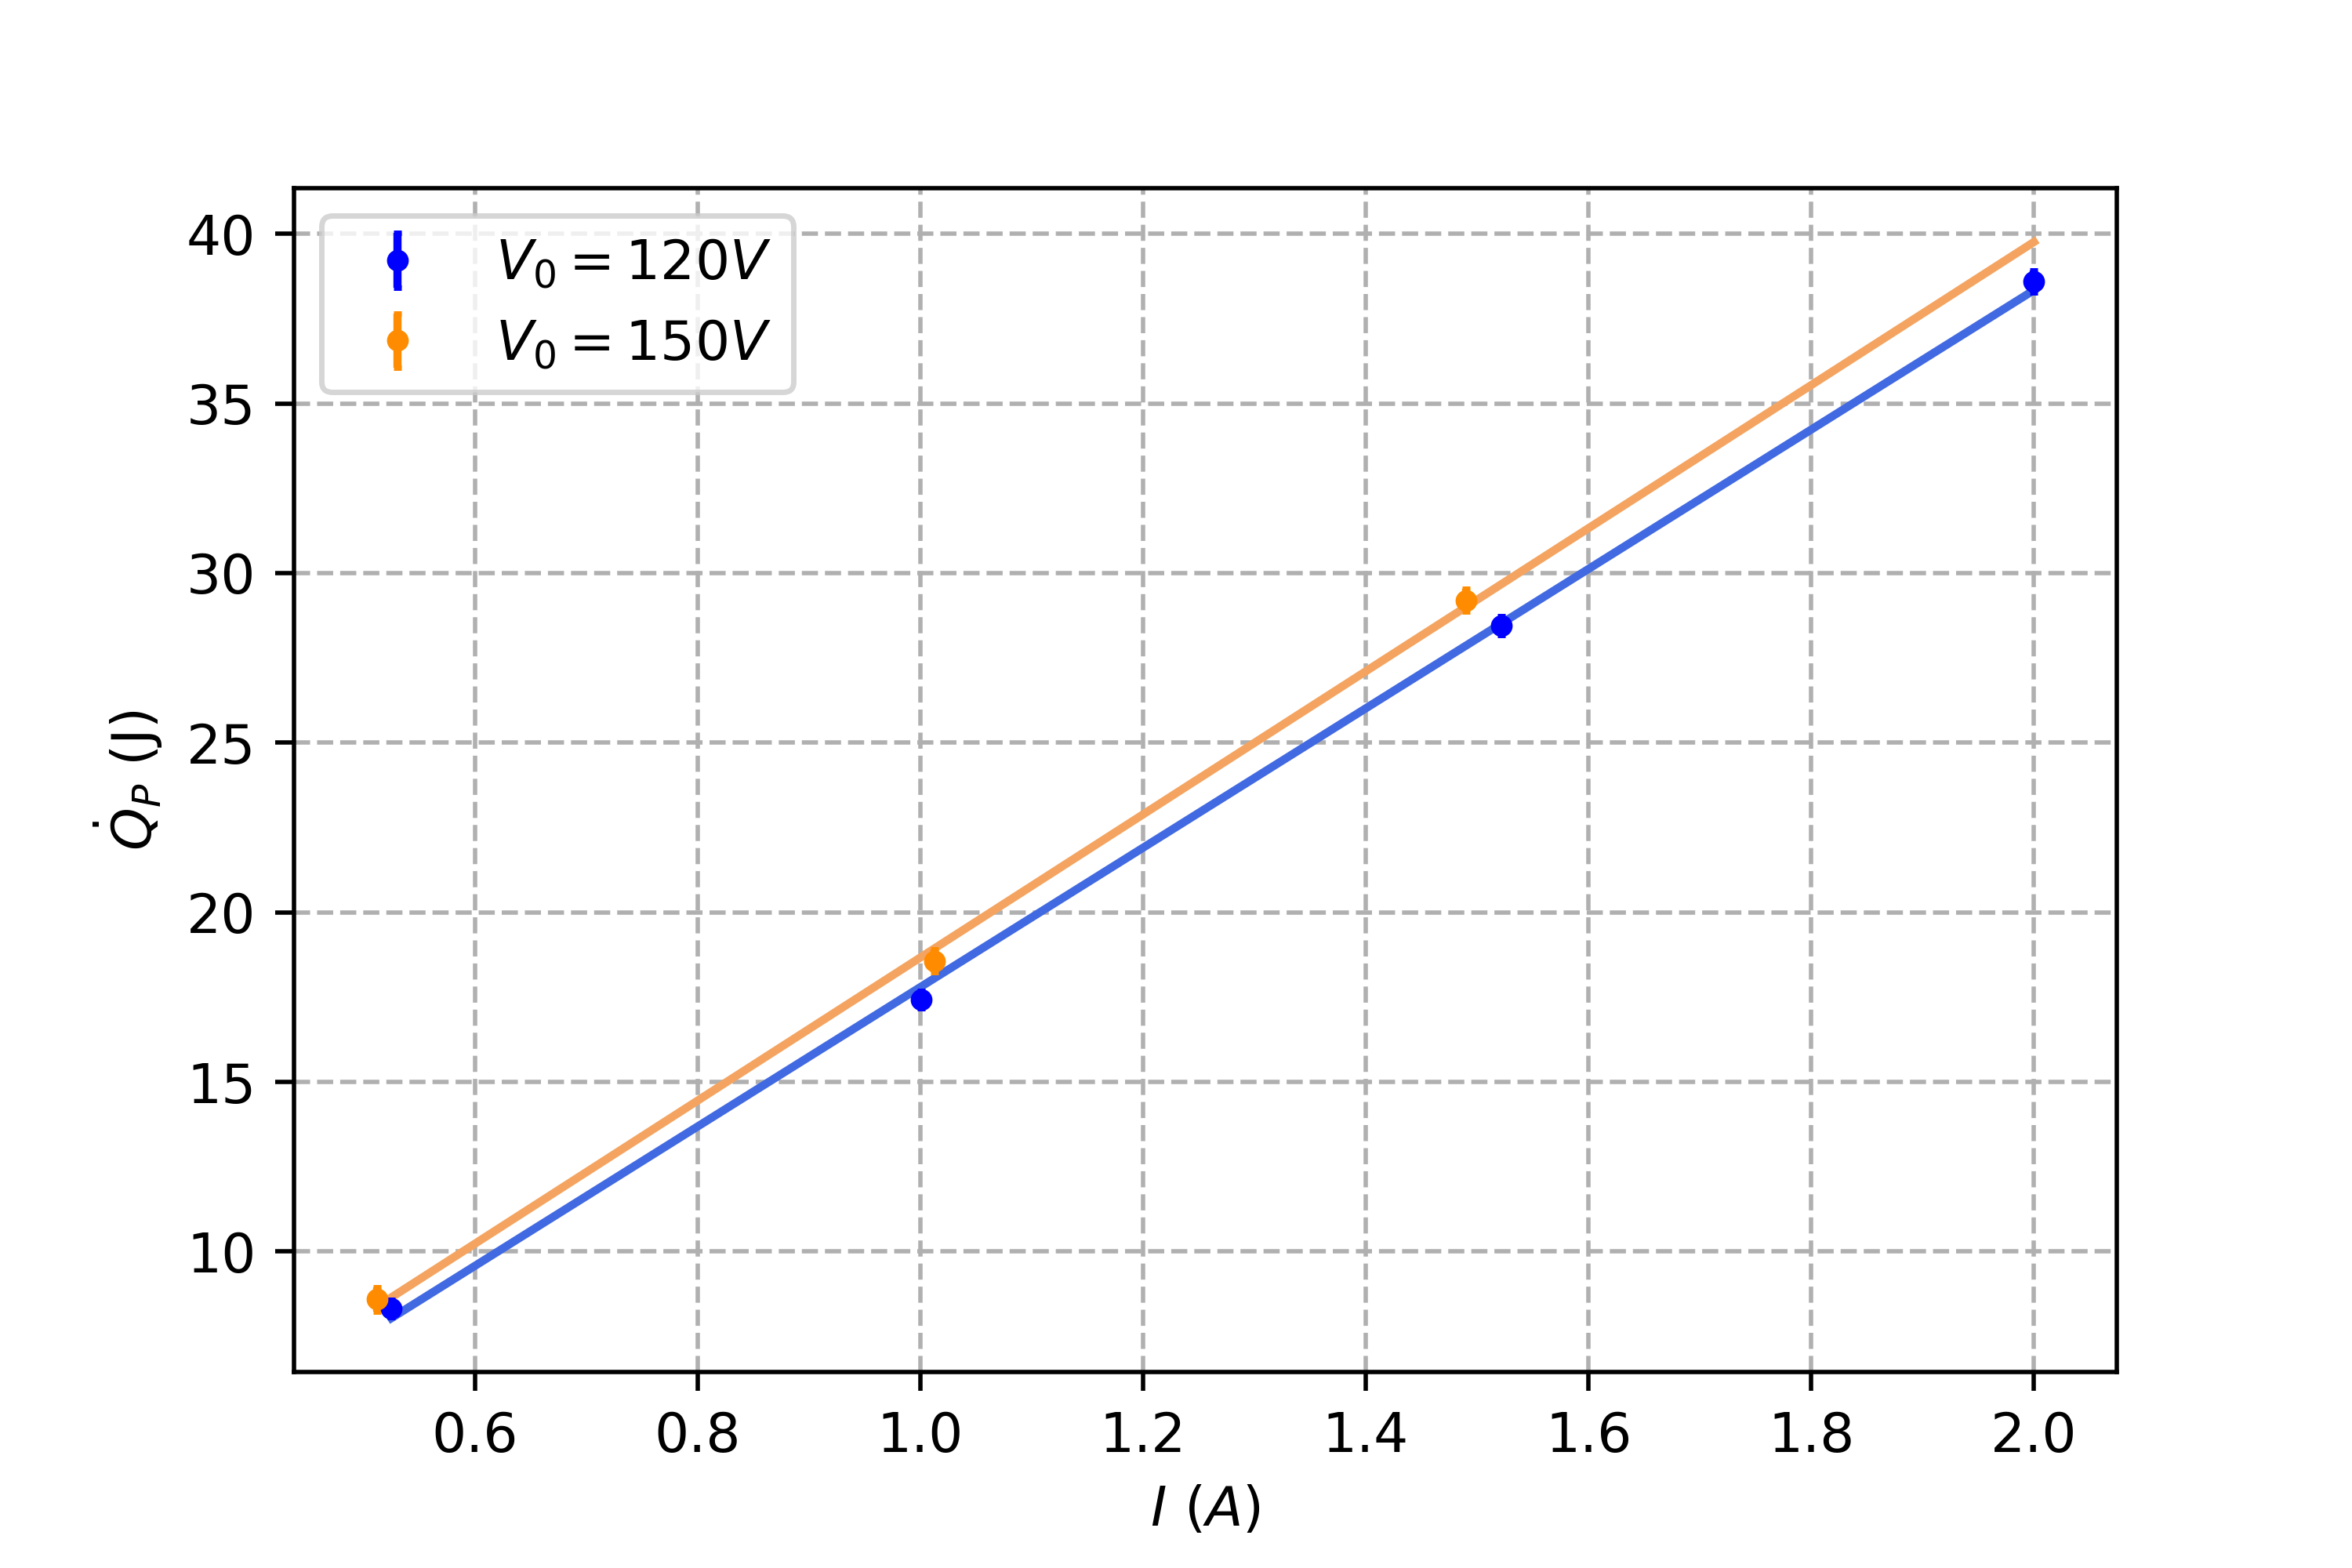
\includegraphics[scale=1]{plot-coeficiente-peltier.png} 
\caption{representación gráfica de los pares de valores ($I,\dot{Q}_P$) para cada voltaje} 
\label{Fig:graficapeltier7}
\end{figure} 



\newpage

\newpage

\section{Conclusión}

El objetivo de la práctica era estudiar los fenómenos termoeléctricos Seebeck y Peltier, calculando el coeficiente Seebeck y Peltier de un dispositivo termoeléctrico formado por diferentes pares (de dos diferentes tipos de semiconductores). Como podemos ver tanto en las tablas \ref{tab:17} y \ref{tab:20}, hemos cumplido dicho objetivo, calculando los valores de los coeficientes. Ahora bien, ¿Hemos cumplido el objetivo de forma plenamente satisfactoria? Vamos a estudiarlo. \\

Comencemos por el coeficiente Seebeck. Está claro que ambos valores están muy próximos entre si, distanciando menos de un 10\% el uno respecto del otro, y dando un valor medio bastante bueno, ya que el valor teórico que debería darnos está en torno a 0.059 $V/K$. Si consideramos que alguno de los termopares ya no está operativo (lo cuál es perfectamente factible dado el tiempo que tiene la práctica), podemos intuir que realmente está muy próximo al valor teórico. En general podemos decir que está parte de la práctica resulta considerablemente buena. De todos modos es importante recalcar que no hemos hecho todo lo bien que podríamos hacerlo, ya que muchas incertidumbres (como la de los polímetros o termómetros) que hemos considerado lineales podrían haber sido tratadas de manera mucho mas rigurosa (viendo las especificaciones del fabricante...), y haber estudiado con mas profundidad las distribuciones de frecuencia para cada valor. \\

Sin duda el coeficiente Peltier es quizás el mejor que los datos, ya que la diferencia entre ellos es poco menos del 5\% entre los valores, y dada la elevada incertidumbre que poseen (y mas si tenemos en cuenta el error $a$ mencionado en el anterior punto), que sean tan similares es todo un éxito. Al igual que con Seebeck, es muy mejorable está práctica (sobretodo en cuanto a incertidumbres), pero una mayor investigación es inviable, además de un exceso, ya que no nos importa tanto la precisión como estudiar fisicamente el fenómeno, y una cosa está clara: existe una clara correlación lineal entre el calor de peltier  y la intensidad que circula el circuito. Lo mismo para la fuerza electromotriz y la diferencia de temperatura entre los puntos del conductor. \\

Además de estos coeficientes termoeléctricos, tuvimos que calcular otros valores (coeficiente de Fourier, capacidad calorífica), que no tuvieron el mismo ratio de éxito. Las capacidades caloríficas de un voltaje a otro cambiaron muchísimo (en torno a un 20\%), lo mismo con los $\lambda_T$. Esto es bastante sorprendente si consideramos que las regresiones son muy buenas, aunque el valor de $C$ varía de la una a la otra; y el error en la toma de datos, copia o posterior cálculo tampoco es probable porque, de ser así, también debería afectar a los valores de los coeficientes, aunque solo tomando mas datos podríamos resolver dicho dilema. Las resistencias (tanto $R_c$ como $r_i$) dan buenos valores, lo cual es bueno. Ocurre lo mismo con la fuerza electromotriz. \\


Otra forma de mejorar la práctica y que personalmente me hubiera gustado es estudiar mejor los comportamientos al variar la potencia, es decir, hacer estudios con mas potenciales, ya que  si nos damos cuenta tanto $S$ como $\pi_{AB}$ aumentaron al aumentar la potencia, y sin embargo $C_a$ descendió. También hay que decir que la temperatura de foco frío no se mantuvo constante en ningún momento, siempre oscilando, ya que al depender del flujo de agua y de la temperatura de está (que varía a lo largo del día) pudo introducir un error. Por ello haber trabajado con un foco mas constante (y reducir esta parte del error) y un flujo también mas constante mejoraría el experimento. \\

Dicho todo esto, podemos concluir la práctica, diciendo que en general, ha sido una buena práctica, con conclusiones bastante satisfactorias, que, por lo menos, no contradicen las ideas de Peltier y Seebeck.


\newpage

\newpage

\section{Datos}
\subsection{Primer día}

\begin{table}[h!] 	 \centering 
\begin{tabular}{|c|c||c|c|} 
\hline 
$ V_{R_c} \ (V)$ & $I \ (A) $ & $ V_{R_c} \ (V)$ & $I \ (A) $  \\ \hline 
20 &  0.022 & 120 & 0.121 \\ 
40  &  0.042 & 140 & 0.14 \\ 
60 &  0.062 & 160 & 0.159 \\ 
80 &  0.082 & 180 & 0.176 \\ 
100 &  0.102 & 200 & 0.195 \\ 
\hline 
\end{tabular} 
\caption{Valores para ($V,I$) para el cálculo de la  resistencia $R_c$} 
\label{tab:} 
\end{table} 



\begin{table}[h!] 	 \centering 
\begin{tabular}{|c|c||c|c|} 
\hline 
$\Delta V_{R_X} \ (V)$ & $I \ (mA) $ & $\Delta V_{R_X} \ (V)$ & $I \ (mA) $  \\ \hline 
0.049 &  100.7 & 0.323 & 65.3 \\ 
0.107 &  92.5 & 0.354 & 61.4 \\ 
0.155 &  86.2 & 0.382 & 58.0 \\ 
0.189 &  81.9 & 0.406 & 55.1 \\ 
0.237 &  75.9 & 0.447 & 50.0 \\ 
0.285 &  70.1 & - & - \\ 
\hline 
\end{tabular} 
\caption{Valores de los pares ($\Delta V_{R_X},I$) para V = 125V} 
\label{tab:} 
\end{table} 

\begin{table}[h!] 	 \centering 
\begin{tabular}{|c|c||c|c|} 
\hline 
$\Delta V_{R_X} \ (V)$ & $I \ (mA) $ & $\Delta V_{R_X} \ (V)$ & $I \ (mA) $  \\ \hline 
0.089 &  140.5 & 0.439 & 94.7 \\ 
0.184 &  125.1 & 0.487 & 89.2 \\ 
0.258 &  118.1 & 0.528 & 84.3 \\ 
0.315 &  111.0 & 0.581 & 77.8 \\ 
0.362 &  104.9 & 0.63 & 71.5 \\ 
0.418 &  98.4 & 0.677 & 65.6 \\ 
\hline 
\end{tabular} 
\caption{Valores de los pares ($\Delta V_{R_X},I$) para V = 150V} 
\label{tab:} 
\end{table} 


\newpage



\begin{table}[h!] 	 \centering 
\begin{tabular}{|c|c|c||c|c|c|} 
\hline 
$T_2 \ (C^o)$ & $T_1 \ (C^o) $ & $t \ (min)$ & $T_2 \ (C^o)$ & $T_1 \ (C^o) $ & $t \ (min)$ \\ \hline 
16.6 &  12.0 & 0 & 26.8 & 12.5 & 30 \\ 
17.1 &  12.0 & 2 & 27.0 & 12.6 & 31 \\ 
18.4 &  12.1 & 4 & 27.2 & 12.6 & 32 \\ 
19.5 &  12.0 & 6 & 27.3 & 12.7 & 33 \\ 
20.7 &  12.1 & 7 & 27.4 & 12.7 & 34 \\ 
21.6 &  12.2 & 8 & 27.6 & 12.7 & 35 \\ 
22.0 &  12.2 & 10 & 27.7 & 12.6 & 36 \\ 
22.7 &  12.0 & 11 & 27.7 & 12.6 & 37 \\ 
23.3 &  12.0 & 15 & 27.8 & 12.5 & 38 \\ 
23.6 &  12.3 & 16 & 27.9 & 12.6 & 39 \\ 
23.9 &  12.4 & 17 & 28.0 & 12.6 & 40 \\ 
24.2 &  12.4 & 18 & 28.1 & 12.6 & 41 \\ 
24.6 &  12.4 & 19 & 28.1 & 12.7 & 42 \\ 
24.9 &  12.5 & 20 & 28.2 & 12.7 & 43 \\ 
25.1 &  12.4 & 21 & 28.3 & 12.7 & 44 \\ 
25.4 &  12.4 & 22 & 28.4 & 12.7 & 45 \\ 
25.6 &  12.4 & 23 & 28.4 & 12.9 & 46 \\ 
25.8 &  12.4 & 24 & 28.5 & 12.9 & 47 \\ 
26.0 &  12.5 & 25 & 28.5 & 12.7 & 48 \\ 
26.2 &  12.5 & 26 & 28.6 & 12.7 & 49 \\ 
26.3 &  12.5 & 27 & 28.6 & 12.7 & 50 \\ 
26.5 &  12.5 & 28 & 28.6 & 12.9 & 51 \\ 
26.7 &  12.5 & 29 & 28.6 & 12.9 & 52 \\ 
\hline 
\end{tabular} 
\caption{Valores ($T_2,T_1,t$) tomados en el laboratorio para voltaje 125$V$} 
\label{tab:} 
\end{table} 



\newpage



\begin{table}[h!] 	 \centering 
\begin{tabular}{|c|c|c||c|c|c|} 
\hline 
$T_2 \ (C^o)$ & $T_1 \ (C^o) $ & $t \ (min)$ & $T_2 \ (C^o)$ & $T_1 \ (C^o) $ & $t \ (min)$ \\ \hline 
28.8 &  13.0 & 0 & 34.6 & 13.5 & 23 \\ 
29.1 &  13.1 & 1 & 34.7 & 13.5 & 24 \\ 
29.5 &  13.1 & 2 & 34.8 & 13.5 & 25 \\ 
29.9 &  13.2 & 3 & 34.9 & 13.5 & 26 \\ 
30.4 &  13.2 & 4 & 34.9 & 13.5 & 27 \\ 
30.8 &  13.3 & 5 & 34.9 & 13.5 & 28 \\ 
31.2 &  13.4 & 6 & 35.0 & 13.5 & 29 \\ 
31.5 &  13.4 & 7 & 35.1 & 13.5 & 30 \\ 
31.9 &  13.5 & 8 & 35.2 & 13.5 & 31 \\ 
32.1 &  13.5 & 9 & 35.2 & 13.5 & 32 \\ 
32.4 &  13.5 & 10 & 35.3 & 13.5 & 33 \\ 
32.7 &  13.5 & 11 & 35.3 & 13.5 & 34 \\ 
32.9 &  13.5 & 12 & 35.4 & 13.5 & 35 \\ 
33.2 &  13.6 & 13 & 35.4 & 13.5 & 36 \\ 
33.4 &  13.6 & 14 & 35.5 & 13.5 & 37 \\ 
33.6 &  13.6 & 15 & 35.5 & 13.5 & 38 \\ 
33.8 &  13.5 & 16 & 35.6 & 13.6 & 39 \\ 
34.0 &  13.5 & 17 & 35.6 & 13.6 & 40 \\ 
34.1 &  13.5 & 18 & 35.7 & 13.7 & 41 \\ 
34.2 &  13.5 & 19 & 35.7 & 13.7 & 42 \\ 
34.3 &  13.5 & 20 & 35.8 & 13.7 & 43 \\ 
34.4 &  13.6 & 21 & 35.8 & 13.6 & 45 \\ 
34.5 &  13.5 & 22 & 35.8 & 13.5 & 46 \\ 
\hline 
\end{tabular} 
\caption{Valores ($T_2,T_1,t$) tomados en el laboratorio para voltaje 150$V$}  
\label{tab:} 
\end{table} 

\newpage

\subsection{Segundo día}

\begin{table}[h!] 	 \centering 
\begin{tabular}{|c|c|c||c|c|c|} 
\hline 
$T_2 \ (C^o)$ & $T_1 \ (C^o) $ & $t \ (min)$ & $T_2 \ (C^o)$ & $T_1 \ (C^o) $ & $t \ (min)$ \\ \hline 
13.8 &  13.8 & 0 & 19.9 & 14.5 & 27 \\ 
14.1 &  13.9 & 2 & 19.9 & 14.5 & 28 \\ 
14.5 &  13.9 & 3 & 20.0 & 14.6 & 29 \\ 
14.9 &  14.0 & 4 & 20.1 & 14.6 & 30 \\ 
15.2 &  14.1 & 5 & 20.4 & 14.6 & 32 \\ 
15.7 &  14.1 & 6 & 20.5 & 14.6 & 33 \\ 
15.9 &  14.2 & 7 & 20.5 & 14.6 & 34 \\ 
16.4 &  14.3 & 8 & 20.6 & 14.5 & 35 \\ 
16.7 &  14.4 & 9 & 20.6 & 14.4 & 36 \\ 
17.0 &  14.4 & 10 & 20.7 & 14.5 & 37 \\ 
17.3 &  14.6 & 11 & 20.8 & 14.5 & 38 \\ 
17.6 &  14.6 & 12 & 20.8 & 14.5 & 39 \\ 
17.8 &  14.6 & 13 & 20.9 & 14.4 & 40 \\ 
17.9 &  14.6 & 14 & 20.9 & 14.5 & 41 \\ 
18.2 &  14.7 & 15 & 21.0 & 14.5 & 42 \\ 
18.5 &  14.8 & 16 & 21.0 & 14.5 & 43 \\ 
18.6 &  14.7 & 17 & 21.1 & 14.5 & 44 \\ 
18.8 &  14.7 & 18 & 21.1 & 14.7 & 45 \\ 
18.9 &  14.7 & 19 & 21.2 & 14.6 & 46 \\ 
19.1 &  14.6 & 20 & 21.1 & 14.6 & 47 \\ 
19.2 &  14.6 & 21 & 21.2 & 14.5 & 48 \\ 
19.3 &  14.5 & 22 & 21.2 & 14.5 & 49 \\ 
19.4 &  14.5 & 23 & 21.3 & 14.6 & 50 \\ 
19.5 &  14.5 & 24 & 21.3 & 14.5 & 51 \\ 
19.7 &  14.6 & 25 & 21.3 & 14.5 & 52 \\ 
19.8 &  14.6 & 26 & 0.0 & 0.0 & 0 \\ 
\hline 
\end{tabular} 
\caption{Valores ($T_2,T_1,t$) tomados en el laboratorio para voltaje 125$V$ e intensidad $0.525 \ A$} 
\label{tab:} 
\end{table} 

\newpage

\begin{table}[h!] 	 \centering 
\begin{tabular}{|c|c|c||c|c|c|} 
\hline 
$T_2 \ (C^o)$ & $T_1 \ (C^o) $ & $t \ (min)$ & $T_2 \ (C^o)$ & $T_1 \ (C^o) $ & $t \ (min)$ \\ \hline 
21.2 &  14.5 & 0 & 17.0 & 15.1 & 14 \\ 
20.2 &  14.5 & 1 & 16.9 & 15.1 & 15 \\ 
19.6 &  15.2 & 2 & 16.8 & 15.1 & 16 \\ 
19.2 &  15.3 & 3 & 16.7 & 15.1 & 18 \\ 
18.9 &  15.3 & 4 & 16.6 & 15.1 & 19 \\ 
18.6 &  15.2 & 5 & 16.4 & 15.1 & 20 \\ 
18.4 &  15.3 & 6 & 16.4 & 15.1 & 21 \\ 
18.2 &  15.2 & 7 & 16.2 & 15.1 & 22 \\ 
17.9 &  15.2 & 8 & 16.1 & 15.1 & 23 \\ 
17.7 &  15.2 & 9 & 16.1 & 15.1 & 24 \\ 
17.6 &  15.0 & 10 & 16.0 & 15.1 & 25 \\ 
17.4 &  15.0 & 11 & 16.0 & 15.1 & 26 \\ 
17.3 &  15.1 & 12 & 16.0 & 15.1 & 27 \\ 
17.1 &  15.2 & 13 & 16.0 & 15.1 & 28 \\ 
\hline 
\end{tabular} 
\caption{Valores ($T_2,T_1,t$) tomados en el laboratorio para voltaje 125$V$ e intensidad $1.001 \ A$} 
\label{tab:} 
\end{table} 

\begin{table}[h!] 	 \centering 
\begin{tabular}{|c|c|c||c|c|c|} 
\hline 
$T_2 \ (C^o)$ & $T_1 \ (C^o) $ & $t \ (min)$ & $T_2 \ (C^o)$ & $T_1 \ (C^o) $ & $t \ (min)$ \\ \hline 
15.5 &  15.3 & 0 & 11.6 & 15.8 & 15 \\ 
14.9 &  16.0 & 1 & 11.5 & 15.8 & 16 \\ 
14.3 &  16.0 & 2 & 11.4 & 15.8 & 17 \\ 
14.0 &  16.1 & 3 & 11.3 & 15.7 & 18 \\ 
13.7 &  16.0 & 4 & 11.2 & 15.7 & 19 \\ 
13.4 &  16.0 & 5 & 11.1 & 15.8 & 20 \\ 
13.1 &  16.0 & 6 & 11.1 & 15.8 & 21 \\ 
13.0 &  15.9 & 7 & 11.0 & 15.8 & 22 \\ 
12.6 &  15.9 & 8 & 10.9 & 15.8 & 23 \\ 
12.4 &  15.9 & 9 & 10.8 & 15.8 & 24 \\ 
12.4 &  15.9 & 10 & 10.8 & 15.8 & 25 \\ 
12.1 &  15.8 & 11 & 10.7 & 15.8 & 26 \\ 
12.0 &  15.8 & 12 & 10.7 & 15.7 & 27 \\ 
11.9 &  15.8 & 13 & 10.7 & 15.8 & 28 \\ 
11.8 &  15.8 & 14 & 0.0 & 0.0 & 0 \\ 
\hline 
\end{tabular} 
\caption{Valores ($T_2,T_1,t$) tomados en el laboratorio para voltaje 125$V$ e intensidad $1.522 \ A$} 
\label{tab:} 
\end{table} 


\newpage


\begin{table}[h!] 	 \centering 
\begin{tabular}{|c|c|c||c|c|c|} 
\hline 
$T_2 \ (C^o)$ & $T_1 \ (C^o) $ & $t \ (min)$ & $T_2 \ (C^o)$ & $T_1 \ (C^o) $ & $t \ (min)$ \\ \hline 
10.3 &  16.0 & 0 & 8.3 & 16.9 & 5 \\ 
9.5 &  16.8 & 1 & 8.2 & 16.9 & 5 \\ 
9.1 &  17.0 & 2 & 8.1 & 16.8 & 6 \\ 
8.8 &  17.1 & 3 & 8.0 & 16.8 & 6 \\ 
8.5 &  17.0 & 4 & 0.0 & 0.0 & 0 \\ 
\hline 
\end{tabular} 
\caption{Valores ($T_2,T_1,t$) tomados en el laboratorio para voltaje 125$V$ e intensidad $2.00 \ A$} 
\label{tab:} 
\end{table} 

\begin{table}[h!] 	 \centering 
\begin{tabular}{|c|c|c||c|c|c|} 
\hline 
$T_2 \ (C^o)$ & $T_1 \ (C^o) $ & $t \ (min)$ & $T_2 \ (C^o)$ & $T_1 \ (C^o) $ & $t \ (min)$ \\ \hline 
12.0 &  13.3 & 0 & 26.2 & 15.1 & 25 \\ 
13.4 &  13.4 & 1 & 26.4 & 15.1 & 26 \\ 
14.5 &  13.7 & 2 & 26.6 & 15.2 & 27 \\ 
15.4 &  13.7 & 3 & 26.8 & 15.1 & 28 \\ 
16.4 &  13.8 & 4 & 27.0 & 15.0 & 29 \\ 
17.2 &  13.8 & 5 & 27.2 & 15.0 & 30 \\ 
18.0 &  14.0 & 6 & 27.4 & 15.0 & 31 \\ 
18.6 &  14.1 & 7 & 27.6 & 15.2 & 32 \\ 
19.2 &  14.3 & 8 & 27.7 & 15.1 & 33 \\ 
19.9 &  14.2 & 9 & 27.8 & 15.2 & 34 \\ 
20.6 &  14.2 & 10 & 28.0 & 15.2 & 35 \\ 
21.1 &  14.4 & 11 & 28.1 & 15.2 & 36 \\ 
21.6 &  14.5 & 12 & 28.2 & 15.2 & 37 \\ 
22.1 &  14.5 & 13 & 28.4 & 15.3 & 38 \\ 
22.5 &  14.6 & 14 & 28.5 & 15.3 & 39 \\ 
22.9 &  14.6 & 15 & 28.6 & 15.4 & 40 \\ 
23.4 &  14.6 & 16 & 28.7 & 15.3 & 41 \\ 
23.6 &  14.7 & 17 & 28.8 & 15.4 & 42 \\ 
24.1 &  14.7 & 18 & 28.9 & 15.4 & 43 \\ 
24.4 &  14.7 & 19 & 29.0 & 15.4 & 44 \\ 
24.8 &  14.8 & 20 & 29.0 & 15.4 & 45 \\ 
24.9 &  14.8 & 21 & 29.1 & 15.4 & 46 \\ 
25.4 &  14.9 & 22 & 29.2 & 15.4 & 47 \\ 
25.7 &  15.0 & 23 & 29.2 & 15.4 & 48 \\ 
26.0 &  15.1 & 24 & 0.0 & 0.0 & 0 \\ 
\hline 
\end{tabular} 
\caption{Valores ($T_2,T_1,t$) tomados en el laboratorio para voltaje 125$V$ e intensidad $A$} 
\label{tab:} 
\end{table} 

\newpage

\begin{table}[h!] 	 \centering 
\begin{tabular}{|c|c|c||c|c|c|} 
\hline 
$T_2 \ (C^o)$ & $T_1 \ (C^o) $ & $t \ (min)$ & $T_2 \ (C^o)$ & $T_1 \ (C^o) $ & $t \ (min)$ \\ \hline 
29.0 &  15.6 & 0 & 25.5 & 16.4 & 15 \\ 
28.3 &  16.4 & 1 & 25.4 & 16.2 & 16 \\ 
27.8 &  16.5 & 2 & 25.3 & 16.2 & 17 \\ 
27.4 &  16.5 & 3 & 25.2 & 16.2 & 18 \\ 
27.1 &  16.5 & 4 & 25.1 & 16.2 & 19 \\ 
27.0 &  16.5 & 5 & 25.0 & 16.2 & 20 \\ 
26.8 &  16.4 & 6 & 25.0 & 16.2 & 21 \\ 
26.6 &  16.4 & 7 & 24.9 & 16.2 & 22 \\ 
26.3 &  16.4 & 8 & 24.8 & 16.1 & 23 \\ 
26.2 &  16.2 & 9 & 24.8 & 16.1 & 24 \\ 
26.0 &  16.2 & 10 & 24.7 & 16.1 & 25 \\ 
25.9 &  16.2 & 11 & 24.7 & 16.2 & 26 \\ 
25.8 &  16.2 & 12 & 24.5 & 16.1 & 27 \\ 
25.7 &  16.2 & 13 & 24.4 & 16.1 & 28 \\ 
25.5 &  16.2 & 14 & 24.4 & 16.2 & 29 \\ 
\hline 
\end{tabular} 
\caption{Valores ($T_2,T_1,t$) tomados en el laboratorio para voltaje 125$V$ e intensidad $1.013 \ A$} 
\label{tab:} 
\end{table} 


\begin{table}[h!] 	 \centering 
\begin{tabular}{|c|c|c||c|c|c|} 
\hline 
$T_2 \ (C^o)$ & $T_1 \ (C^o) $ & $t \ (min)$ & $T_2 \ (C^o)$ & $T_1 \ (C^o) $ & $t \ (min)$ \\ \hline 
24.2 &  16.9 & 0 & 20.1 & 17.2 & 17 \\ 
24.0 &  16.9 & 1 & 20.0 & 17.2 & 18 \\ 
22.9 &  17.4 & 2 & 20.0 & 17.2 & 19 \\ 
22.6 &  17.4 & 3 & 19.9 & 17.2 & 20 \\ 
22.3 &  17.4 & 4 & 19.9 & 17.2 & 21 \\ 
22.0 &  17.3 & 5 & 19.8 & 17.2 & 22 \\ 
21.8 &  17.3 & 6 & 19.7 & 17.2 & 23 \\ 
21.6 &  17.2 & 7 & 19.6 & 17.2 & 24 \\ 
21.5 &  17.3 & 8 & 19.5 & 17.2 & 25 \\ 
21.3 &  17.2 & 9 & 19.4 & 17.2 & 26 \\ 
21.1 &  17.2 & 10 & 19.4 & 17.1 & 27 \\ 
21.0 &  17.2 & 11 & 19.3 & 17.2 & 28 \\ 
20.8 &  17.3 & 12 & 19.3 & 17.0 & 29 \\ 
20.7 &  17.3 & 13 & 19.2 & 16.9 & 30 \\ 
20.6 &  17.3 & 14 & 19.2 & 16.9 & 31 \\ 
20.4 &  17.3 & 15 & 19.2 & 16.9 & 32 \\ 
20.3 &  17.2 & 16 & 0.0 & 0.0 & 0 \\ 
\hline 
\end{tabular} 
\caption{Valores ($T_2,T_1,t$) tomados en el laboratorio para voltaje 125$V$ e intensidad $1.502A$} 
\label{tab:} 
\end{table} 


\begin{table}[h!] 	 \centering 
\begin{tabular}{|c|c|c|c|c|c|} 
\hline 
$A \ (C^o)$ & $s(A) \ (C^o)$ & $ B  \ (C^o)$ & $s(B) \ (C^o)$ & $C \ (\mathrm{min}^{-1}) $&  $s(C) \ (\mathrm{min}^{-1}) $ \\ \hline 
21.775221  & 0.003000 &  -8.412728 & 0.003300 & 0.055884 & 0.000001 \\ 
\hline
\end{tabular} 
\caption{Valores del ajuste exponencial para $V_0 = 120 V$ e $I = 0.525 A$} 
\label{tab:} 
\end{table} 
 

\newpage
 
 
\begin{table}[h!] 	 \centering 
\begin{tabular}{|c|c|c|c|c|c|} 
\hline 
$A \ (C^o)$ & $s(A) \ (C^o)$ & $ B  \ (C^o)$ & $s(B) \ (C^o)$ & $C \ (\mathrm{min}^{-1}) $&  $s(C) \ (\mathrm{min}^{-1}) $ \\ \hline 
15.767466  & 0.009300 &  4.995179 & 0.010000 & 0.104656 & 0.000040 \\ 
\hline
\end{tabular} 
\caption{Valores del ajuste exponencial para $V_0 = 120 V$ e $I = 1.001 A$} 
\label{tab:} 
\end{table} 
 
 
 
 
\begin{table}[h!] 	 \centering 
\begin{tabular}{|c|c|c|c|c|c|} 
\hline 
$A \ (C^o)$ & $s(A) \ (C^o)$ & $ B  \ (C^o)$ & $s(B) \ (C^o)$ & $C \ (\mathrm{min}^{-1}) $&  $s(C) \ (\mathrm{min}^{-1}) $ \\ \hline 
10.347455  & 0.004300 &  4.956257 & 0.003700 & 0.093529 & 0.000012 \\ 
\hline
\end{tabular} 
\caption{Valores del ajuste exponencial para $V_0 = 120 V$ e $I = 1.522 A$} 
\label{tab:} 
\end{table} 
 
 
 
 
\begin{table}[h!] 	 \centering 
\begin{tabular}{|c|c|c|c|c|c|} 
\hline 
$A \ (C^o)$ & $s(A) \ (C^o)$ & $ B  \ (C^o)$ & $s(B) \ (C^o)$ & $C \ (\mathrm{min}^{-1}) $&  $s(C) \ (\mathrm{min}^{-1}) $ \\ \hline 
7.648912  & 0.017000 &  2.599763 & 0.014000 & 0.287077 & 0.001100 \\ 
\hline
\end{tabular} 
\caption{Valores del ajuste exponencial para $V_0 = 120 V$ e $I = 2.000 A$} 
\label{tab:} 
\end{table} 
 
 
 
 
\begin{table}[h!] 	 \centering 
\begin{tabular}{|c|c|c|c|c|c|} 
\hline 
$A \ (C^o)$ & $s(A) \ (C^o)$ & $ B  \ (C^o)$ & $s(B) \ (C^o)$ & $C \ (\mathrm{min}^{-1}) $&  $s(C) \ (\mathrm{min}^{-1}) $ \\ \hline 
30.170666  & 0.003400 &  -17.737908 & 0.003500 & 0.060058 & 0.000000 \\ 
\hline
\end{tabular} 
\caption{Valores del ajuste exponencial para $V_0 = 150 V$ e $I = 0.512 A$} 
\label{tab:} 
\end{table} 
 
 
 
 
\begin{table}[h!] 	 \centering 
\begin{tabular}{|c|c|c|c|c|c|} 
\hline 
$A \ (C^o)$ & $s(A) \ (C^o)$ & $ B  \ (C^o)$ & $s(B) \ (C^o)$ & $C \ (\mathrm{min}^{-1}) $&  $s(C) \ (\mathrm{min}^{-1}) $ \\ \hline 
24.238308  & 0.009800 &  4.413459 & 0.008500 & 0.089707 & 0.000033 \\ 
\hline
\end{tabular} 
\caption{Valores del ajuste exponencial para $V_0 = 150 V$ e $I = 1.013 A$} 
\label{tab:} 
\end{table} 
 
 
 
 
\begin{table}[h!] 	 \centering 
\begin{tabular}{|c|c|c|c|c|c|} 
\hline 
$A \ (C^o)$ & $s(A) \ (C^o)$ & $ B  \ (C^o)$ & $s(B) \ (C^o)$ & $C \ (\mathrm{min}^{-1}) $&  $s(C) \ (\mathrm{min}^{-1}) $ \\ \hline 
18.924071  & 0.011000 &  5.050366 & 0.011000 & 0.085228 & 0.000028 \\ 
\hline
\end{tabular} 
\caption{Valores del ajuste exponencial para $V_0 = 150 V$ e $I = 1.490 A$} 
\label{tab:} 
\end{table} 

\newpage

\section{Anexo \label{sec:anexo}}

En la siguiente figura tenemos un montaje de los elementos del laboratorio para el cálculo del coeficiente seebeck. Son los mismos elementos que hemos mencionado en el subapartado de material, pero aquí vamos a mostrarlos. Tenemos que:

\begin{enumerate}
\item Dispositivo termoeléctrico. Aunque no se vea, dentro de la caja está nuestro dispositivo termoeléctrico, formado por 142 termopares de semiconductores de tipo n y p. En general la diferencia entre ambos es como trasmiten la electricidad: uno trasmite electricidad mediante electrones (portadores de carga negativos) y el otro mediante huecos (huecos electrónicos, portadores de carga positivos). La diferencia está en que ambos semiconductores tienen densidades electrónicas diferentes debido a esta forma de trasmitir la carga: uno será aceptor y otro dador.

\item Bornes del dispositivo. En estas regiones podemos conectar los polímetros (o lo que sea) para calcular el potencial generado por el efecto Seebeck.

\item Tubos de agua. Permiten refrigerar la unión fría y mantenerla a temperatura constante.

\item Resistencia calefactora. La usamos para aumentar la temperatura de la unión caliente, y así tener una diferencia de temperatura lo suficientemente grande como para que aparezca un potencial observable. Usa el efecto Joule para calentar el dispositivo. Siempre estará conectada a 5. por cables.
 
\item  Generador de corriente alterna. Aportará la potencia necesaria a nuestra resistencia calefactora para que aumente la temperatura. Usamos corriente alterna debido a su eficiencia a la hora de trasmitir grandes voltajes.

\item Termómetro digital. Mide la temperatura de la unión fría y caliente en cada momento. 

\item Polímetro. 

\item Polímetro.

\item Resistencia variable que podremos controlar accionando la rueda 11. Por cada vuelta aumentará $10 \Omega$ la resistencia, hata $100 \Omega$, aunque no será necesario llegar a dicha cantidad. 

\item Bornes mediante los cuales conectaremos los cables para el montaje de la imagen 

\end{enumerate}
 
\newpage

\begin{figure}[h!] \centering
\includegraphics[scale=0.58]{foto1.png}
\caption{montaje para la toma de datos de la temperatura.}
\label{Fig:foto1}
\end{figure}


\newpage

En la figura siguiente mostramos el montaje experimental llevado acabo para calcular la resistencia $R_c$. Como podemos ver tenemos la resistencia conectada por los cables 1-2 al generador, y por 3-4 a un polímetro conectado en serie, por lo que podemos intuir que actuará como un amperímetro. Luego el 5-6 volverá al generador, cerrando el circuito. Además podemos ver un polímetro conectado en paralelo a los bornes del generador, por lo que actuará como un voltímetro. Es muy importante conectar bien los bornes del polímetro, ya que es muy probable que salten chispas o entren en contacto, provocando un cortocircuito y romper el fusible del voltímetro. Recordemos que también calculamos $R_c$ conectando los cables 2-3 directamente a un polímetro y seleccionando la parte de ohmnímetro.

\begin{figure}[h!] \centering
\includegraphics[scale=1.0]{foto3.png}
\caption{montaje experimental para el cálculo de $R_c$.}
\label{Fig:foto3}
\end{figure}

\newpage

En la siguiente figura tenemos el montaje para la toma de datos para la evolución de la temperatura. Tenemos conectada la resistencia $R_c$ al generador, y un voltímetro en paralelo que nos indique constantemente la potencia que trasmite el generador. Además tenemos el termómetro, y donde aparecen ambas temperaturas.

\begin{figure}[h!] \centering
\includegraphics[scale=0.80]{foto4.png}
\caption{montaje experimental para la toma de datos de la temperatura.}
\label{Fig:foto4}
\end{figure}


En la siguiente imagen podemos ver un voltímetro conectado en serie a los bornes del dispositivo termoeléctrico, para tomar directamente la potencia. No importa si 3-4 y 1-2 o 2-3 y 4-1, solo cambiará el signo del potencial. 


\begin{figure}[h!] \centering
\includegraphics[scale=0.75]{foto5.png}
\caption{montaje experimental para la toma de $\varepsilon$ directamente.}
\label{Fig:foto5}
\end{figure}

\newpage

Tenemos que uno de los bornes del dispositivo están conectados de 1-2 a un amperímetro (por eso en serie) midiendo la intensidad del circuito en todo momento. Luego el circuito se cierra conectando el amperímetro a la resistencia variable $R_v$ 3-4 y está otra vez al borne del dispositivo 5-6. Además tendremos un voltímetro conectado a la resistencia variable (en paralelo a esta) que medirá la diferencia de potencial entre los dos puntos de la resistencia en cada momento (mediante 7-8 y 9-10). 

\begin{figure}[h!] \centering
\includegraphics[scale=0.6]{foto6.png}
\caption{montaje experimental para el cálculo de $\varepsilon$ indirectamente.}
\label{Fig:foto6}
\end{figure} 

En la figura siguiente \ref{Fig:foto7} vemos el material necesario para calcular el calor de Peltier y el coeficiente de Peltier. Muchos elementos ya los conocemos porque han sido mencionados en la figura \ref{Fig:foto1}. Solo introduciremos uno:

\begin{itemize}
\item \textbf{1.} Es nuestro generador de corriente continua que conectaremos mediante \textbf{2.} a los bornes  del dispositivo (3.) con un amperímetro conectado en serie. Es importante no cambiar la posición de los cables una vez hemos encontrado el sentido correcto, ya que cambia el sentido de la corriente y por tanto del calor.
\end{itemize}

El montaje final debe quedar como en la figura \ref{Fig:foto8}. 

\begin{figure}[h!] \centering
\includegraphics[scale=0.60]{foto7.png}
\caption{elementos para obtener las evoluciones de la temperatura para Peltier}
\label{Fig:foto7}
\end{figure}


\begin{figure}[h!] \centering
\includegraphics[scale=0.48]{foto8.png}
\caption{montaje para obtener las evoluciones de la temperatura para Peltier}
\label{Fig:foto8}
\end{figure}



\end{document}
